\documentclass[10pt,a4paper]{article}

\usepackage[italian]{babel}
\usepackage{amsmath}
\usepackage{amsfonts}
\usepackage{amssymb}

\usepackage[left=1cm,right=1cm,top=1cm,bottom=2cm]{geometry}

\usepackage{txfonts}
\usepackage[T1]{fontenc}
\usepackage[utf8]{inputenc}

\usepackage{titlesec}
\setcounter{secnumdepth}{4}
\titleformat{\subsection}{\normalfont\fontsize{13}{13}\bfseries}{\thesubsection}{1em}{}
\titleformat{\subsubsection}{\normalfont\fontsize{11}{11}\bfseries}{\thesubsubsection}{1em}{}
\titleformat{\paragraph}{\normalfont\normalsize\bfseries}{\theparagraph}{1em}{}
\titlespacing*{\paragraph}{0pt}{3.25ex plus 1ex minus .2ex}{1.5ex plus .2ex}

%per le immagini
\usepackage{graphicx}
\usepackage{subcaption}
\usepackage{wrapfig}

%per i link
\usepackage{hyperref} 

%%%%%%%% per il codice c++
\usepackage{textcomp}
\usepackage{listings}          % for creating language style
\usepackage{listingsutf8}
 %%%%%%%%%%%%%%%%%%%%%%%%%%%%%%%%%%%%%%%%%%%%%%%%%%%%%%%%%%%%%%%%%%%%%%%%%%%%%%%% 
%%% ~ Arduino Language - Arduino IDE Colors ~                                  %%%
%%%                                                                            %%%
%%% Kyle Rocha-Brownell | 10/2/2017 | No Licence                               %%%
%%% -------------------------------------------------------------------------- %%%
%%%                                                                            %%%
%%% Place this file in your working directory (next to the latex file you're   %%%
%%% working on).  To add it to your project, place:                            %%%
%%%     %%%%%%%%%%%%%%%%%%%%%%%%%%%%%%%%%%%%%%%%%%%%%%%%%%%%%%%%%%%%%%%%%%%%%%%%%%%%%%%% 
%%% ~ Arduino Language - Arduino IDE Colors ~                                  %%%
%%%                                                                            %%%
%%% Kyle Rocha-Brownell | 10/2/2017 | No Licence                               %%%
%%% -------------------------------------------------------------------------- %%%
%%%                                                                            %%%
%%% Place this file in your working directory (next to the latex file you're   %%%
%%% working on).  To add it to your project, place:                            %%%
%%%     %%%%%%%%%%%%%%%%%%%%%%%%%%%%%%%%%%%%%%%%%%%%%%%%%%%%%%%%%%%%%%%%%%%%%%%%%%%%%%%% 
%%% ~ Arduino Language - Arduino IDE Colors ~                                  %%%
%%%                                                                            %%%
%%% Kyle Rocha-Brownell | 10/2/2017 | No Licence                               %%%
%%% -------------------------------------------------------------------------- %%%
%%%                                                                            %%%
%%% Place this file in your working directory (next to the latex file you're   %%%
%%% working on).  To add it to your project, place:                            %%%
%%%    \input{arduinoLanguage.tex}                                             %%%
%%% somewhere before \begin{document} in your latex file.                      %%%
%%%                                                                            %%%
%%% In your document, place your arduino code between:                         %%%
%%%   \begin{lstlisting}[language=Arduino]                                     %%%
%%% and:                                                                       %%%
%%%   \end{lstlisting}                                                         %%%
%%%                                                                            %%%
%%% Or create your own style to add non-built-in functions and variables.      %%%
%%%                                                                            %%%
 %%%%%%%%%%%%%%%%%%%%%%%%%%%%%%%%%%%%%%%%%%%%%%%%%%%%%%%%%%%%%%%%%%%%%%%%%%%%%%%% 

\usepackage{color}
\usepackage{listings}    
\usepackage{courier}
\usepackage{listingsutf8}

%%% Define Custom IDE Colors %%%
\definecolor{arduinoGreen}    {rgb} {0.17, 0.43, 0.01}
\definecolor{arduinoGrey}     {rgb} {0.47, 0.47, 0.33}
\definecolor{arduinoOrange}   {rgb} {0.8 , 0.4 , 0   }
\definecolor{arduinoBlue}     {rgb} {0.01, 0.61, 0.98}
\definecolor{arduinoDarkBlue} {rgb} {0.0 , 0.2 , 0.5 }
\definecolor{light-gray}{gray}{0.95}

%%% Define Arduino Language %%%
\lstdefinelanguage{Arduino}{
  language=C++, % begin with default C++ settings 
%
%
  %%% Keyword Color Group 1 %%%  (called KEYWORD3 by arduino)
  keywordstyle=\color{arduinoGreen},   
  deletekeywords={  % remove all arduino keywords that might be in c++
                break, case, override, final, continue, default, do, else, for, 
                if, return, goto, switch, throw, try, while, setup, loop, export, 
                not, or, and, xor, include, define, elif, else, error, if, ifdef, 
                ifndef, pragma, warning,
                HIGH, LOW, INPUT, INPUT_PULLUP, OUTPUT, DEC, BIN, HEX, OCT, PI, 
                HALF_PI, TWO_PI, LSBFIRST, MSBFIRST, CHANGE, FALLING, RISING, 
                DEFAULT, EXTERNAL, INTERNAL, INTERNAL1V1, INTERNAL2V56, LED_BUILTIN, 
                LED_BUILTIN_RX, LED_BUILTIN_TX, DIGITAL_MESSAGE, FIRMATA_STRING, 
                ANALOG_MESSAGE, REPORT_DIGITAL, REPORT_ANALOG, SET_PIN_MODE, 
                SYSTEM_RESET, SYSEX_START, auto, int8_t, int16_t, int32_t, int64_t, 
                uint8_t, uint16_t, uint32_t, uint64_t, char16_t, char32_t, operator, 
                enum, delete, bool, boolean, byte, char, const, false, float, double, 
                null, NULL, int, long, new, private, protected, public, short, 
                signed, static, volatile, String, void, true, unsigned, word, array, 
                sizeof, dynamic_cast, typedef, const_cast, struct, static_cast, union, 
                friend, extern, class, reinterpret_cast, register, explicit, inline, 
                _Bool, complex, _Complex, _Imaginary, atomic_bool, atomic_char, 
                atomic_schar, atomic_uchar, atomic_short, atomic_ushort, atomic_int, 
                atomic_uint, atomic_long, atomic_ulong, atomic_llong, atomic_ullong, 
                virtual, PROGMEM,
                Serial, Serial1, Serial2, Serial3, SerialUSB, Keyboard, Mouse,
                abs, acos, asin, atan, atan2, ceil, constrain, cos, degrees, exp, 
                floor, log, map, max, min, radians, random, randomSeed, round, sin, 
                sq, sqrt, tan, pow, bitRead, bitWrite, bitSet, bitClear, bit, 
                highByte, lowByte, analogReference, analogRead, 
                analogReadResolution, analogWrite, analogWriteResolution, 
                attachInterrupt, detachInterrupt, digitalPinToInterrupt, delay, 
                delayMicroseconds, digitalWrite, digitalRead, interrupts, millis, 
                micros, noInterrupts, noTone, pinMode, pulseIn, pulseInLong, shiftIn, 
                shiftOut, tone, yield, Stream, begin, end, peek, read, print, 
                println, available, availableForWrite, flush, setTimeout, find, 
                findUntil, parseInt, parseFloat, readBytes, readBytesUntil, readString, 
                readStringUntil, trim, toUpperCase, toLowerCase, charAt, compareTo, 
                concat, endsWith, startsWith, equals, equalsIgnoreCase, getBytes, 
                indexOf, lastIndexOf, length, replace, setCharAt, substring, 
                toCharArray, toInt, press, release, releaseAll, accept, click, move, 
                isPressed, isAlphaNumeric, isAlpha, isAscii, isWhitespace, isControl, 
                isDigit, isGraph, isLowerCase, isPrintable, isPunct, isSpace, 
                isUpperCase, isHexadecimalDigit, 
                }, 
  morekeywords={   % add arduino structures to group 1
                break, case, override, final, continue, default, do, else, for, 
                if, return, goto, switch, throw, try, while, setup, loop, export, 
                not, or, and, xor, include, define, elif, else, error, if, ifdef, 
                ifndef, pragma, warning,
                }, 
% 
%
  %%% Keyword Color Group 2 %%%  (called LITERAL1 by arduino)
  keywordstyle=[2]\color{arduinoBlue},   
  keywords=[2]{   % add variables and dataTypes as 2nd group  
                HIGH, LOW, INPUT, INPUT_PULLUP, OUTPUT, DEC, BIN, HEX, OCT, PI, 
                HALF_PI, TWO_PI, LSBFIRST, MSBFIRST, CHANGE, FALLING, RISING, 
                DEFAULT, EXTERNAL, INTERNAL, INTERNAL1V1, INTERNAL2V56, LED_BUILTIN, 
                LED_BUILTIN_RX, LED_BUILTIN_TX, DIGITAL_MESSAGE, FIRMATA_STRING, 
                ANALOG_MESSAGE, REPORT_DIGITAL, REPORT_ANALOG, SET_PIN_MODE, 
                SYSTEM_RESET, SYSEX_START, auto, int8_t, int16_t, int32_t, int64_t, 
                uint8_t, uint16_t, uint32_t, uint64_t, char16_t, char32_t, operator, 
                enum, delete, bool, boolean, byte, char, const, false, float, double, 
                null, NULL, int, long, new, private, protected, public, short, 
                signed, static, volatile, String, void, true, unsigned, word, array, 
                sizeof, dynamic_cast, typedef, const_cast, struct, static_cast, union, 
                friend, extern, class, reinterpret_cast, register, explicit, inline, 
                _Bool, complex, _Complex, _Imaginary, atomic_bool, atomic_char, 
                atomic_schar, atomic_uchar, atomic_short, atomic_ushort, atomic_int, 
                atomic_uint, atomic_long, atomic_ulong, atomic_llong, atomic_ullong, 
                virtual, PROGMEM,
                },  
% 
%
  %%% Keyword Color Group 3 %%%  (called KEYWORD1 by arduino)
  keywordstyle=[3]\bfseries\color{arduinoOrange},
  keywords=[3]{  % add built-in functions as a 3rd group
                Serial, Serial1, Serial2, Serial3, SerialUSB, Keyboard, Mouse,
                },      
%
%
  %%% Keyword Color Group 4 %%%  (called KEYWORD2 by arduino)
  keywordstyle=[4]\color{arduinoOrange},
  keywords=[4]{  % add more built-in functions as a 4th group
                abs, acos, asin, atan, atan2, ceil, constrain, cos, degrees, exp, 
                floor, log, map, max, min, radians, random, randomSeed, round, sin, 
                sq, sqrt, tan, pow, bitRead, bitWrite, bitSet, bitClear, bit, 
                highByte, lowByte, analogReference, analogRead, 
                analogReadResolution, analogWrite, analogWriteResolution, 
                attachInterrupt, detachInterrupt, digitalPinToInterrupt, delay, 
                delayMicroseconds, digitalWrite, digitalRead, interrupts, millis, 
                micros, noInterrupts, noTone, pinMode, pulseIn, pulseInLong, shiftIn, 
                shiftOut, tone, yield, Stream, begin, end, peek, read, print, 
                println, available, availableForWrite, flush, setTimeout, find, 
                findUntil, parseInt, parseFloat, readBytes, readBytesUntil, readString, 
                readStringUntil, trim, toUpperCase, toLowerCase, charAt, compareTo, 
                concat, endsWith, startsWith, equals, equalsIgnoreCase, getBytes, 
                indexOf, lastIndexOf, length, replace, setCharAt, substring, 
                toCharArray, toInt, press, release, releaseAll, accept, click, move, 
                isPressed, isAlphaNumeric, isAlpha, isAscii, isWhitespace, isControl, 
                isDigit, isGraph, isLowerCase, isPrintable, isPunct, isSpace, 
                isUpperCase, isHexadecimalDigit, 
                },      
%
  extendedchars=true,
%
  %%% Set Other Colors %%%
  stringstyle=\color{arduinoDarkBlue},
  showstringspaces=false,  
  commentstyle=\color{arduinoGrey},    
%          
%   
  %%%% Line Numbering %%%%
  numbers=left,                    
  numbersep=5pt,                   
  numberstyle=\color{arduinoGrey},    
  %stepnumber=2,                      % show every 2 line numbers
%
%
  %%%% Code Box Style %%%%
  breaklines=true,                    % wordwrapping
  tabsize=2,         
  basicstyle=\fontsize{9}{11}\ttfamily,
  backgroundcolor=\color{light-gray},
  xleftmargin=.35in
}                                             %%%
%%% somewhere before \begin{document} in your latex file.                      %%%
%%%                                                                            %%%
%%% In your document, place your arduino code between:                         %%%
%%%   \begin{lstlisting}[language=Arduino]                                     %%%
%%% and:                                                                       %%%
%%%   \end{lstlisting}                                                         %%%
%%%                                                                            %%%
%%% Or create your own style to add non-built-in functions and variables.      %%%
%%%                                                                            %%%
 %%%%%%%%%%%%%%%%%%%%%%%%%%%%%%%%%%%%%%%%%%%%%%%%%%%%%%%%%%%%%%%%%%%%%%%%%%%%%%%% 

\usepackage{color}
\usepackage{listings}    
\usepackage{courier}
\usepackage{listingsutf8}

%%% Define Custom IDE Colors %%%
\definecolor{arduinoGreen}    {rgb} {0.17, 0.43, 0.01}
\definecolor{arduinoGrey}     {rgb} {0.47, 0.47, 0.33}
\definecolor{arduinoOrange}   {rgb} {0.8 , 0.4 , 0   }
\definecolor{arduinoBlue}     {rgb} {0.01, 0.61, 0.98}
\definecolor{arduinoDarkBlue} {rgb} {0.0 , 0.2 , 0.5 }
\definecolor{light-gray}{gray}{0.95}

%%% Define Arduino Language %%%
\lstdefinelanguage{Arduino}{
  language=C++, % begin with default C++ settings 
%
%
  %%% Keyword Color Group 1 %%%  (called KEYWORD3 by arduino)
  keywordstyle=\color{arduinoGreen},   
  deletekeywords={  % remove all arduino keywords that might be in c++
                break, case, override, final, continue, default, do, else, for, 
                if, return, goto, switch, throw, try, while, setup, loop, export, 
                not, or, and, xor, include, define, elif, else, error, if, ifdef, 
                ifndef, pragma, warning,
                HIGH, LOW, INPUT, INPUT_PULLUP, OUTPUT, DEC, BIN, HEX, OCT, PI, 
                HALF_PI, TWO_PI, LSBFIRST, MSBFIRST, CHANGE, FALLING, RISING, 
                DEFAULT, EXTERNAL, INTERNAL, INTERNAL1V1, INTERNAL2V56, LED_BUILTIN, 
                LED_BUILTIN_RX, LED_BUILTIN_TX, DIGITAL_MESSAGE, FIRMATA_STRING, 
                ANALOG_MESSAGE, REPORT_DIGITAL, REPORT_ANALOG, SET_PIN_MODE, 
                SYSTEM_RESET, SYSEX_START, auto, int8_t, int16_t, int32_t, int64_t, 
                uint8_t, uint16_t, uint32_t, uint64_t, char16_t, char32_t, operator, 
                enum, delete, bool, boolean, byte, char, const, false, float, double, 
                null, NULL, int, long, new, private, protected, public, short, 
                signed, static, volatile, String, void, true, unsigned, word, array, 
                sizeof, dynamic_cast, typedef, const_cast, struct, static_cast, union, 
                friend, extern, class, reinterpret_cast, register, explicit, inline, 
                _Bool, complex, _Complex, _Imaginary, atomic_bool, atomic_char, 
                atomic_schar, atomic_uchar, atomic_short, atomic_ushort, atomic_int, 
                atomic_uint, atomic_long, atomic_ulong, atomic_llong, atomic_ullong, 
                virtual, PROGMEM,
                Serial, Serial1, Serial2, Serial3, SerialUSB, Keyboard, Mouse,
                abs, acos, asin, atan, atan2, ceil, constrain, cos, degrees, exp, 
                floor, log, map, max, min, radians, random, randomSeed, round, sin, 
                sq, sqrt, tan, pow, bitRead, bitWrite, bitSet, bitClear, bit, 
                highByte, lowByte, analogReference, analogRead, 
                analogReadResolution, analogWrite, analogWriteResolution, 
                attachInterrupt, detachInterrupt, digitalPinToInterrupt, delay, 
                delayMicroseconds, digitalWrite, digitalRead, interrupts, millis, 
                micros, noInterrupts, noTone, pinMode, pulseIn, pulseInLong, shiftIn, 
                shiftOut, tone, yield, Stream, begin, end, peek, read, print, 
                println, available, availableForWrite, flush, setTimeout, find, 
                findUntil, parseInt, parseFloat, readBytes, readBytesUntil, readString, 
                readStringUntil, trim, toUpperCase, toLowerCase, charAt, compareTo, 
                concat, endsWith, startsWith, equals, equalsIgnoreCase, getBytes, 
                indexOf, lastIndexOf, length, replace, setCharAt, substring, 
                toCharArray, toInt, press, release, releaseAll, accept, click, move, 
                isPressed, isAlphaNumeric, isAlpha, isAscii, isWhitespace, isControl, 
                isDigit, isGraph, isLowerCase, isPrintable, isPunct, isSpace, 
                isUpperCase, isHexadecimalDigit, 
                }, 
  morekeywords={   % add arduino structures to group 1
                break, case, override, final, continue, default, do, else, for, 
                if, return, goto, switch, throw, try, while, setup, loop, export, 
                not, or, and, xor, include, define, elif, else, error, if, ifdef, 
                ifndef, pragma, warning,
                }, 
% 
%
  %%% Keyword Color Group 2 %%%  (called LITERAL1 by arduino)
  keywordstyle=[2]\color{arduinoBlue},   
  keywords=[2]{   % add variables and dataTypes as 2nd group  
                HIGH, LOW, INPUT, INPUT_PULLUP, OUTPUT, DEC, BIN, HEX, OCT, PI, 
                HALF_PI, TWO_PI, LSBFIRST, MSBFIRST, CHANGE, FALLING, RISING, 
                DEFAULT, EXTERNAL, INTERNAL, INTERNAL1V1, INTERNAL2V56, LED_BUILTIN, 
                LED_BUILTIN_RX, LED_BUILTIN_TX, DIGITAL_MESSAGE, FIRMATA_STRING, 
                ANALOG_MESSAGE, REPORT_DIGITAL, REPORT_ANALOG, SET_PIN_MODE, 
                SYSTEM_RESET, SYSEX_START, auto, int8_t, int16_t, int32_t, int64_t, 
                uint8_t, uint16_t, uint32_t, uint64_t, char16_t, char32_t, operator, 
                enum, delete, bool, boolean, byte, char, const, false, float, double, 
                null, NULL, int, long, new, private, protected, public, short, 
                signed, static, volatile, String, void, true, unsigned, word, array, 
                sizeof, dynamic_cast, typedef, const_cast, struct, static_cast, union, 
                friend, extern, class, reinterpret_cast, register, explicit, inline, 
                _Bool, complex, _Complex, _Imaginary, atomic_bool, atomic_char, 
                atomic_schar, atomic_uchar, atomic_short, atomic_ushort, atomic_int, 
                atomic_uint, atomic_long, atomic_ulong, atomic_llong, atomic_ullong, 
                virtual, PROGMEM,
                },  
% 
%
  %%% Keyword Color Group 3 %%%  (called KEYWORD1 by arduino)
  keywordstyle=[3]\bfseries\color{arduinoOrange},
  keywords=[3]{  % add built-in functions as a 3rd group
                Serial, Serial1, Serial2, Serial3, SerialUSB, Keyboard, Mouse,
                },      
%
%
  %%% Keyword Color Group 4 %%%  (called KEYWORD2 by arduino)
  keywordstyle=[4]\color{arduinoOrange},
  keywords=[4]{  % add more built-in functions as a 4th group
                abs, acos, asin, atan, atan2, ceil, constrain, cos, degrees, exp, 
                floor, log, map, max, min, radians, random, randomSeed, round, sin, 
                sq, sqrt, tan, pow, bitRead, bitWrite, bitSet, bitClear, bit, 
                highByte, lowByte, analogReference, analogRead, 
                analogReadResolution, analogWrite, analogWriteResolution, 
                attachInterrupt, detachInterrupt, digitalPinToInterrupt, delay, 
                delayMicroseconds, digitalWrite, digitalRead, interrupts, millis, 
                micros, noInterrupts, noTone, pinMode, pulseIn, pulseInLong, shiftIn, 
                shiftOut, tone, yield, Stream, begin, end, peek, read, print, 
                println, available, availableForWrite, flush, setTimeout, find, 
                findUntil, parseInt, parseFloat, readBytes, readBytesUntil, readString, 
                readStringUntil, trim, toUpperCase, toLowerCase, charAt, compareTo, 
                concat, endsWith, startsWith, equals, equalsIgnoreCase, getBytes, 
                indexOf, lastIndexOf, length, replace, setCharAt, substring, 
                toCharArray, toInt, press, release, releaseAll, accept, click, move, 
                isPressed, isAlphaNumeric, isAlpha, isAscii, isWhitespace, isControl, 
                isDigit, isGraph, isLowerCase, isPrintable, isPunct, isSpace, 
                isUpperCase, isHexadecimalDigit, 
                },      
%
  extendedchars=true,
%
  %%% Set Other Colors %%%
  stringstyle=\color{arduinoDarkBlue},
  showstringspaces=false,  
  commentstyle=\color{arduinoGrey},    
%          
%   
  %%%% Line Numbering %%%%
  numbers=left,                    
  numbersep=5pt,                   
  numberstyle=\color{arduinoGrey},    
  %stepnumber=2,                      % show every 2 line numbers
%
%
  %%%% Code Box Style %%%%
  breaklines=true,                    % wordwrapping
  tabsize=2,         
  basicstyle=\fontsize{9}{11}\ttfamily,
  backgroundcolor=\color{light-gray},
  xleftmargin=.35in
}                                             %%%
%%% somewhere before \begin{document} in your latex file.                      %%%
%%%                                                                            %%%
%%% In your document, place your arduino code between:                         %%%
%%%   \begin{lstlisting}[language=Arduino]                                     %%%
%%% and:                                                                       %%%
%%%   \end{lstlisting}                                                         %%%
%%%                                                                            %%%
%%% Or create your own style to add non-built-in functions and variables.      %%%
%%%                                                                            %%%
 %%%%%%%%%%%%%%%%%%%%%%%%%%%%%%%%%%%%%%%%%%%%%%%%%%%%%%%%%%%%%%%%%%%%%%%%%%%%%%%% 

\usepackage{color}
\usepackage{listings}    
\usepackage{courier}
\usepackage{listingsutf8}

%%% Define Custom IDE Colors %%%
\definecolor{arduinoGreen}    {rgb} {0.17, 0.43, 0.01}
\definecolor{arduinoGrey}     {rgb} {0.47, 0.47, 0.33}
\definecolor{arduinoOrange}   {rgb} {0.8 , 0.4 , 0   }
\definecolor{arduinoBlue}     {rgb} {0.01, 0.61, 0.98}
\definecolor{arduinoDarkBlue} {rgb} {0.0 , 0.2 , 0.5 }
\definecolor{light-gray}{gray}{0.95}

%%% Define Arduino Language %%%
\lstdefinelanguage{Arduino}{
  language=C++, % begin with default C++ settings 
%
%
  %%% Keyword Color Group 1 %%%  (called KEYWORD3 by arduino)
  keywordstyle=\color{arduinoGreen},   
  deletekeywords={  % remove all arduino keywords that might be in c++
                break, case, override, final, continue, default, do, else, for, 
                if, return, goto, switch, throw, try, while, setup, loop, export, 
                not, or, and, xor, include, define, elif, else, error, if, ifdef, 
                ifndef, pragma, warning,
                HIGH, LOW, INPUT, INPUT_PULLUP, OUTPUT, DEC, BIN, HEX, OCT, PI, 
                HALF_PI, TWO_PI, LSBFIRST, MSBFIRST, CHANGE, FALLING, RISING, 
                DEFAULT, EXTERNAL, INTERNAL, INTERNAL1V1, INTERNAL2V56, LED_BUILTIN, 
                LED_BUILTIN_RX, LED_BUILTIN_TX, DIGITAL_MESSAGE, FIRMATA_STRING, 
                ANALOG_MESSAGE, REPORT_DIGITAL, REPORT_ANALOG, SET_PIN_MODE, 
                SYSTEM_RESET, SYSEX_START, auto, int8_t, int16_t, int32_t, int64_t, 
                uint8_t, uint16_t, uint32_t, uint64_t, char16_t, char32_t, operator, 
                enum, delete, bool, boolean, byte, char, const, false, float, double, 
                null, NULL, int, long, new, private, protected, public, short, 
                signed, static, volatile, String, void, true, unsigned, word, array, 
                sizeof, dynamic_cast, typedef, const_cast, struct, static_cast, union, 
                friend, extern, class, reinterpret_cast, register, explicit, inline, 
                _Bool, complex, _Complex, _Imaginary, atomic_bool, atomic_char, 
                atomic_schar, atomic_uchar, atomic_short, atomic_ushort, atomic_int, 
                atomic_uint, atomic_long, atomic_ulong, atomic_llong, atomic_ullong, 
                virtual, PROGMEM,
                Serial, Serial1, Serial2, Serial3, SerialUSB, Keyboard, Mouse,
                abs, acos, asin, atan, atan2, ceil, constrain, cos, degrees, exp, 
                floor, log, map, max, min, radians, random, randomSeed, round, sin, 
                sq, sqrt, tan, pow, bitRead, bitWrite, bitSet, bitClear, bit, 
                highByte, lowByte, analogReference, analogRead, 
                analogReadResolution, analogWrite, analogWriteResolution, 
                attachInterrupt, detachInterrupt, digitalPinToInterrupt, delay, 
                delayMicroseconds, digitalWrite, digitalRead, interrupts, millis, 
                micros, noInterrupts, noTone, pinMode, pulseIn, pulseInLong, shiftIn, 
                shiftOut, tone, yield, Stream, begin, end, peek, read, print, 
                println, available, availableForWrite, flush, setTimeout, find, 
                findUntil, parseInt, parseFloat, readBytes, readBytesUntil, readString, 
                readStringUntil, trim, toUpperCase, toLowerCase, charAt, compareTo, 
                concat, endsWith, startsWith, equals, equalsIgnoreCase, getBytes, 
                indexOf, lastIndexOf, length, replace, setCharAt, substring, 
                toCharArray, toInt, press, release, releaseAll, accept, click, move, 
                isPressed, isAlphaNumeric, isAlpha, isAscii, isWhitespace, isControl, 
                isDigit, isGraph, isLowerCase, isPrintable, isPunct, isSpace, 
                isUpperCase, isHexadecimalDigit, 
                }, 
  morekeywords={   % add arduino structures to group 1
                break, case, override, final, continue, default, do, else, for, 
                if, return, goto, switch, throw, try, while, setup, loop, export, 
                not, or, and, xor, include, define, elif, else, error, if, ifdef, 
                ifndef, pragma, warning,
                }, 
% 
%
  %%% Keyword Color Group 2 %%%  (called LITERAL1 by arduino)
  keywordstyle=[2]\color{arduinoBlue},   
  keywords=[2]{   % add variables and dataTypes as 2nd group  
                HIGH, LOW, INPUT, INPUT_PULLUP, OUTPUT, DEC, BIN, HEX, OCT, PI, 
                HALF_PI, TWO_PI, LSBFIRST, MSBFIRST, CHANGE, FALLING, RISING, 
                DEFAULT, EXTERNAL, INTERNAL, INTERNAL1V1, INTERNAL2V56, LED_BUILTIN, 
                LED_BUILTIN_RX, LED_BUILTIN_TX, DIGITAL_MESSAGE, FIRMATA_STRING, 
                ANALOG_MESSAGE, REPORT_DIGITAL, REPORT_ANALOG, SET_PIN_MODE, 
                SYSTEM_RESET, SYSEX_START, auto, int8_t, int16_t, int32_t, int64_t, 
                uint8_t, uint16_t, uint32_t, uint64_t, char16_t, char32_t, operator, 
                enum, delete, bool, boolean, byte, char, const, false, float, double, 
                null, NULL, int, long, new, private, protected, public, short, 
                signed, static, volatile, String, void, true, unsigned, word, array, 
                sizeof, dynamic_cast, typedef, const_cast, struct, static_cast, union, 
                friend, extern, class, reinterpret_cast, register, explicit, inline, 
                _Bool, complex, _Complex, _Imaginary, atomic_bool, atomic_char, 
                atomic_schar, atomic_uchar, atomic_short, atomic_ushort, atomic_int, 
                atomic_uint, atomic_long, atomic_ulong, atomic_llong, atomic_ullong, 
                virtual, PROGMEM,
                },  
% 
%
  %%% Keyword Color Group 3 %%%  (called KEYWORD1 by arduino)
  keywordstyle=[3]\bfseries\color{arduinoOrange},
  keywords=[3]{  % add built-in functions as a 3rd group
                Serial, Serial1, Serial2, Serial3, SerialUSB, Keyboard, Mouse,
                },      
%
%
  %%% Keyword Color Group 4 %%%  (called KEYWORD2 by arduino)
  keywordstyle=[4]\color{arduinoOrange},
  keywords=[4]{  % add more built-in functions as a 4th group
                abs, acos, asin, atan, atan2, ceil, constrain, cos, degrees, exp, 
                floor, log, map, max, min, radians, random, randomSeed, round, sin, 
                sq, sqrt, tan, pow, bitRead, bitWrite, bitSet, bitClear, bit, 
                highByte, lowByte, analogReference, analogRead, 
                analogReadResolution, analogWrite, analogWriteResolution, 
                attachInterrupt, detachInterrupt, digitalPinToInterrupt, delay, 
                delayMicroseconds, digitalWrite, digitalRead, interrupts, millis, 
                micros, noInterrupts, noTone, pinMode, pulseIn, pulseInLong, shiftIn, 
                shiftOut, tone, yield, Stream, begin, end, peek, read, print, 
                println, available, availableForWrite, flush, setTimeout, find, 
                findUntil, parseInt, parseFloat, readBytes, readBytesUntil, readString, 
                readStringUntil, trim, toUpperCase, toLowerCase, charAt, compareTo, 
                concat, endsWith, startsWith, equals, equalsIgnoreCase, getBytes, 
                indexOf, lastIndexOf, length, replace, setCharAt, substring, 
                toCharArray, toInt, press, release, releaseAll, accept, click, move, 
                isPressed, isAlphaNumeric, isAlpha, isAscii, isWhitespace, isControl, 
                isDigit, isGraph, isLowerCase, isPrintable, isPunct, isSpace, 
                isUpperCase, isHexadecimalDigit, 
                },      
%
  extendedchars=true,
%
  %%% Set Other Colors %%%
  stringstyle=\color{arduinoDarkBlue},
  showstringspaces=false,  
  commentstyle=\color{arduinoGrey},    
%          
%   
  %%%% Line Numbering %%%%
  numbers=left,                    
  numbersep=5pt,                   
  numberstyle=\color{arduinoGrey},    
  %stepnumber=2,                      % show every 2 line numbers
%
%
  %%%% Code Box Style %%%%
  breaklines=true,                    % wordwrapping
  tabsize=2,         
  basicstyle=\fontsize{9}{11}\ttfamily,
  backgroundcolor=\color{light-gray},
  xleftmargin=.35in
}    % adds the arduino language listing
\definecolor{commentgreen}    {RGB}{2,112,10}
\definecolor{eminence}        {RGB}{108,48,130}
\definecolor{weborange}       {RGB}{255,165,0}
\definecolor{frenchplum}      {RGB}{129,20,83}


%% Define an Arduino style fore use later %%
\lstdefinestyle{myArduino}
{
  language=Arduino,
    %% Add other words needing highlighting below %%
    morekeywords=[1]{},                  % [1] -> dark green
    morekeywords=[2]{FILE_WRITE},        % [2] -> light blue
    morekeywords=[3]{SD, File},          % [3] -> bold orange
    morekeywords=[4]{open, exists, write, SoftwareSerial},      % [4] -> orange
    frame=tb,    
    inputencoding=utf8,
    extendedchars=true,
    literate={è}{{\`{e}}}{1},
    breaklines=true,  
}

\lstdefinestyle{mycpp}
{
    language=C++,
    inputencoding=utf8,
    extendedchars=true,
    literate={è}{{\`{e}}}{1},
    %escapeinside={(*******}{*******)}
    escapechar=\£,
    %escapeinside=~~,
    frame=tb,
    tabsize=2,
    mathescape=false,
    breaklines=true,                    % wordwrapping
    postbreak=\mbox{\textcolor{red}{$\hookrightarrow$}\space},         
    basicstyle=\fontsize{9}{11}\ttfamily,
    backgroundcolor=\color{light-gray},
    xleftmargin=.25in,
    showstringspaces=false,
    numbers=left,                    
    numbersep=5pt,                   
    %numberstyle=\color{arduinoGrey},    
    %stepnumber=2, 
    %upquote=true,
    commentstyle=\color{commentgreen},
    keywordstyle=\color{eminence},
    stringstyle=\color{red},
    basicstyle=\small\ttfamily, % basic font setting
    emph={int,char,double,float,unsigned,void,bool},
    emphstyle={\color{blue}},
    % keyword highlighting
    classoffset=1, % starting new class
    otherkeywords={>,<,.,;,-,!,=,~},
    morekeywords={>,<,.,;,-,!,=,~},
    keywordstyle=\color{weborange},
    classoffset=0,
}

\lstdefinestyle{mycuda}
{
    language=C++,
    inputencoding=utf8,
    extendedchars=true,
     literate=
    {á}{{\'a}}1 {é}{{\'e}}1 {í}{{\'i}}1 {ó}{{\'o}}1 {ú}{{\'u}}1
    {Á}{{\'A}}1 {É}{{\'E}}1 {Í}{{\'I}}1 {Ó}{{\'O}}1 {Ú}{{\'U}}1
    {à}{{\`a}}1 {è}{{\`e}}1 {ì}{{\`i}}1 {ò}{{\`o}}1 {ù}{{\`u}}1
    {À}{{\`A}}1 {È}{{\'E}}1 {Ì}{{\`I}}1 {Ò}{{\`O}}1 {Ù}{{\`U}}1
    {ä}{{\"a}}1 {ë}{{\"e}}1 {ï}{{\"i}}1 {ö}{{\"o}}1 {ü}{{\"u}}1
    {Ä}{{\"A}}1 {Ë}{{\"E}}1 {Ï}{{\"I}}1 {Ö}{{\"O}}1 {Ü}{{\"U}}1
    {â}{{\^a}}1 {ê}{{\^e}}1 {î}{{\^i}}1 {ô}{{\^o}}1 {û}{{\^u}}1
    {Â}{{\^A}}1 {Ê}{{\^E}}1 {Î}{{\^I}}1 {Ô}{{\^O}}1 {Û}{{\^U}}1
    {œ}{{\oe}}1 {Œ}{{\OE}}1 {æ}{{\ae}}1 {Æ}{{\AE}}1 {ß}{{\ss}}1
    {ç}{{\c c}}1 {Ç}{{\c C}}1 {ø}{{\o}}1 {å}{{\r a}}1 {Å}{{\r A}}1
    {€}{{\EUR}}1 {£}{{\pounds}}1,
    %escapeinside={(*******}{*******)}
    escapechar=\£,
    %escapeinside=~~,
    frame=tb,
    tabsize=2,
    mathescape=false,
    breaklines=true,                    % wordwrapping
    postbreak=\mbox{\textcolor{red}{$\hookrightarrow$}\space},         
    basicstyle=\fontsize{9}{11}\ttfamily,
    backgroundcolor=\color{light-gray},
    xleftmargin=.25in,
    showstringspaces=false,
    numbers=left,                    
    numbersep=5pt,                   
    %numberstyle=\color{arduinoGrey},    
    %stepnumber=2, 
    %upquote=true,
    commentstyle=\color{commentgreen},
    keywordstyle=\color{eminence},
    stringstyle=\color{red},
    basicstyle=\small\ttfamily, % basic font setting
    emph={int,char,double,float,unsigned,void,bool},
    emphstyle={\color{blue}},
    morekeywords = [2]{cudaMalloc, cudaFree,
        __global__, __shared__, __device__, __host__,
        __syncthreads},
    keywordstyle=[2]\color{magenta},
    % keyword highlighting
    classoffset=1, % starting new class
    otherkeywords={>,<,.,;,-,!,=,~},
    morekeywords=[3]{>,<,.,;,-,!,=,~zz},
    keywordstyle=[3]\color{weborange},
    classoffset=0,
}

\lstdefinestyle{mycsharp}
{
    language=[Sharp]C,
    inputencoding=utf8,
    extendedchars=true,
     literate=
    {á}{{\'a}}1 {é}{{\'e}}1 {í}{{\'i}}1 {ó}{{\'o}}1 {ú}{{\'u}}1
    {Á}{{\'A}}1 {É}{{\'E}}1 {Í}{{\'I}}1 {Ó}{{\'O}}1 {Ú}{{\'U}}1
    {à}{{\`a}}1 {è}{{\`e}}1 {ì}{{\`i}}1 {ò}{{\`o}}1 {ù}{{\`u}}1
    {À}{{\`A}}1 {È}{{\'E}}1 {Ì}{{\`I}}1 {Ò}{{\`O}}1 {Ù}{{\`U}}1
    {ä}{{\"a}}1 {ë}{{\"e}}1 {ï}{{\"i}}1 {ö}{{\"o}}1 {ü}{{\"u}}1
    {Ä}{{\"A}}1 {Ë}{{\"E}}1 {Ï}{{\"I}}1 {Ö}{{\"O}}1 {Ü}{{\"U}}1
    {â}{{\^a}}1 {ê}{{\^e}}1 {î}{{\^i}}1 {ô}{{\^o}}1 {û}{{\^u}}1
    {Â}{{\^A}}1 {Ê}{{\^E}}1 {Î}{{\^I}}1 {Ô}{{\^O}}1 {Û}{{\^U}}1
    {œ}{{\oe}}1 {Œ}{{\OE}}1 {æ}{{\ae}}1 {Æ}{{\AE}}1 {ß}{{\ss}}1
    {ç}{{\c c}}1 {Ç}{{\c C}}1 {ø}{{\o}}1 {å}{{\r a}}1 {Å}{{\r A}}1
    {€}{{\EUR}}1 {£}{{\pounds}}1,
    %escapeinside={(*******}{*******)}
    escapechar=\£,
    %escapeinside=~~,
    frame=tb,
    tabsize=2,
    mathescape=false,
    breaklines=true,                    % wordwrapping
    postbreak=\mbox{\textcolor{red}{$\hookrightarrow$}\space},         
    basicstyle=\fontsize{9}{11}\ttfamily,
    backgroundcolor=\color{light-gray},
    xleftmargin=.25in,
    showstringspaces=false,
    numbers=left,                    
    numbersep=5pt,                   
    %numberstyle=\color{arduinoGrey},    
    %stepnumber=2, 
    %upquote=true,
    commentstyle=\color{commentgreen},
    keywordstyle=\color{eminence},
    stringstyle=\color{red},
    basicstyle=\small\ttfamily, % basic font setting
    emph={int,char,double,float,unsigned,void,bool,byte},
    emphstyle={\color{blue}},
    % keyword highlighting
    classoffset=1, % starting new class
    otherkeywords={>,<,.,;,-,!,=,~},
    morekeywords=[3]{>,<,.,;,-,!,=,~zz},
    keywordstyle=[3]\color{weborange},
    classoffset=0,
}


\lstdefinestyle{myoutput}
{
    inputencoding=utf8,
    extendedchars=true,
    literate={è}{{\`{e}}}{1},
    tabsize=2,
    frame=tb,
    breaklines=true,                    % wordwrapping
    postbreak=\mbox{\textcolor{red}{$\hookrightarrow$}\space},         
    basicstyle=\fontsize{9}{11}\ttfamily,
    backgroundcolor=\color{light-gray},
    xleftmargin=.25in,
    showstringspaces=false,
    numbers=left,                    
    numbersep=5pt, 
}
%%%%%%%%%%%%%%%%%%%%%%%


\usepackage{siunitx} %pacchetto per le unita' di misura

%%%%%%%%%%%%%%%%%%%%%% per i flowchart
\usepackage{xcolor}
\usepackage{tikz}
\usetikzlibrary{shapes,arrows}
\usetikzlibrary{arrows.meta}
\usetikzlibrary{positioning}
\usetikzlibrary{shapes.geometric}
\usepgflibrary{shapes.symbols}
\usetikzlibrary{shapes.multipart}
\usetikzlibrary{decorations.pathreplacing}

\tikzset{%
  >={Latex[width=2mm,length=2mm]},
  % Specifications for style of nodes:
            rect/.style = {rectangle, rounded corners, draw=black,
                           minimum width=4cm, minimum height=1cm,
                           text centered, font=\sffamily},
           round/.style = {ellipse, draw, draw=black,
                           minimum width=4cm, minimum height=1cm,
                           text centered, font=\sffamily},
       smallrect/.style = {rectangle, rounded corners, draw=black,
                           minimum width=2cm, minimum height=1cm,
                           text centered, font=\sffamily},
 smallrectsplit4/.style = {rectangle split, rectangle split parts=4, 
	                       rectangle split part fill={green!30, none, none, none},
	                       align=center,
	                       rounded corners, draw=black,
                           minimum width=2cm, minimum height=1cm,
                           text centered, font=\sffamily},
        rectpile/.style = {rectangle, outer sep=0pt, align=right,
                           minimum width=1cm, minimum height=0.5cm, font=\sffamily}
}

%\tikzset{%
%    >={Latex[width=2mm,length=2mm]},
%      % Specifications for style of nodes:
%         declare/.style = {trapezium,draw=black, minimum width=4cm, minimum height=1cm, 
%                                trapezium right angle=-70, trapezium left angle=70,
%                                minimum width=4cm, minimum height=1cm,
%                                text centered, font=\sffamily},
%           start/.style = {ellipse, draw, draw=black, minimum width=4cm, 
%                                minimum height=1cm, text centered, font=\sffamily},
%            cond/.style = {diamond, aspect=2, draw, draw=black,
%                                minimum width=4cm, minimum height=1cm,
%                                text centered, font=\sffamily},
%            rect/.style = {rectangle, draw, draw=black,
%                                minimum width=4cm, minimum height=1cm,
%                                text centered, font=\sffamily},
%}
%%%%%%%%%%%%%%%%%%%%%%%%%%%%%%%%%%%%%%%
% 

\pagenumbering{arabic}
\pagestyle{plain}

% per non farlo anadre a capo ovunque 
% va in conflitto con quello che lo fa andare a capo nel codice quindi attenzione <--------
%\usepackage[none]{hyphenat}
\usepackage[italian=nohyphenation,english=nohyphenation]{hyphsubst}

% per togliere gli ident all'inizio dei paragrafi
\setlength{\parindent}{0pt}






\begin{document}

\section{Prefazione}
 
\subsection{scopo del progetto}
L'obbiettivo di questo progetto \`e la realizzazione di una modello di machine learning in grado di apprendere le relazioni tra i dati fruiti da una scheda embeded dotata di accelerometro, giroscopio e magnetometro, e la posizione spaziale di un braccio umano.
Il problema che ci si \`e posti di risolvere poteva essere risolto in modo deterministico ma per lo scopo del progetto si voleva risolvere il problema tramite un algoritmo di ML, per poter verificare l'efficacia di questo metodo per la risoluzione di un problema con soluzione nota.


\subsection{introduzione generale alle tecniche utilizzate}
Per la realizzazione del progetto è stata realizzata una scheda con microcontrollore arduino, provvista di bluetooth, accelerometro, magnetometro, alimentata a batteria.
\'E stata realizzata una libreria in C++/CUDA per la creazione, l'addestramento e l'utilizzo di una rete neuronale con supporto per CPU e GPU.
\'E stato realizzato un secondo programma C++, per l'acquisizione dei dati della scheda e per l'acquisizione dei punti dello scheletro forniti dal kinect, lo stesso programma si occupa della sincronizzazione di tali dati e della creazione di un dataset necessario per il processo di addestramento della rete neuronale.
In fine è stato realizzato un programma C\# che sfrutta il game engine Unity per la realizzazione dell'ambiente grafico, che rende possibile la visualizzazione dell'output della rete, muovendo un manichino secondo gli input della scheda.
Quest'ultima operazione è stata effettuata mettendo in comunicazione il programma C++ che si occuppa dell'acquisizione dei dati della scheda, e che ne esegue l'input nel modello addestrato, per poi passare i dati elaborati tramite comunicazione socket interna al motore grafico.       

\section{Richiami di teoria}
\subsection{Dal machine learning al deep learning}
Oggi l'intelligenza artificiale è un fiorente campo di ricerca, con l'obiettivo di risolvere una grande varietà di problemi, che per essere risolti attraverso la programmazione classica necessitano di una grande quantità di conoscenze pregresse, spesso non disponibili.\\
I Programmi basati sul paradigma dell'intelligenza artificiale si propongono di superare questi ostacoli acquisendo direttamente queste conoscenze dai dati grezzi, tale capacità è nota come machine learning.
Sotto questa famiglia di algoritmi si trovano altri sottogruppi quali il representation learning e all'interno di quest'ultimo il deep learning.\\ 
Il deep learning rispetto ai metodi più classici, tipicamente in grado di riconoscere relazioni lineari(come ad esempio il noto SVM o support vector machine), si propone come alternativa per l'apprendimento di funzioni a molte variabili non lineari anche molto complesse.
Le applicazioni più comuni comprendono il riconoscimento di oggetti nelle immagini, delle parole in tracce audio o anche per le traduzioni multilingue. \\
Il termine "deep learning" deriva proprio dalla capacità di questi modelli di riuscire a cogliere delle relazioni molto "profonde" tra i dati di ingresso e di uscita, approssimando con un certo errore ,dipendente dal caso specifico, la funzione che dati gli input restituisce l'output desiderato, purtroppo però presentano il grande problema di non rendere disponibile in maniera chiara le relazioni apprese.
   

\begin{figure}[h!]
  \centering
  \begin{subfigure}[t]{0.45\linewidth}
  	\centering
    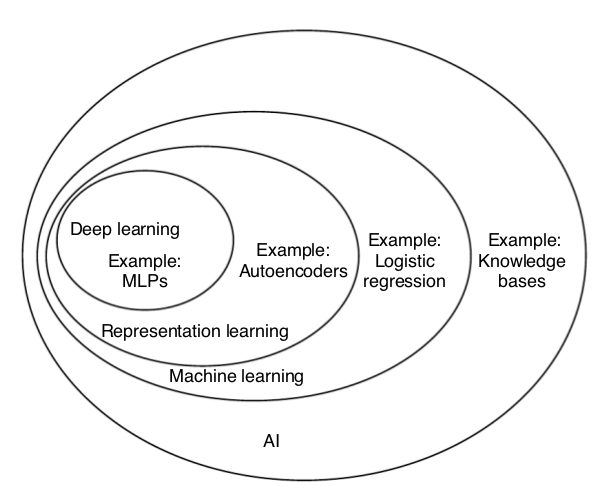
\includegraphics[height=200pt]{AI_venn_diagram.png}
    \caption*{famiglie di algoritmi}
  \end{subfigure}
  \begin{subfigure}[t]{0.45\linewidth}
  	\centering
    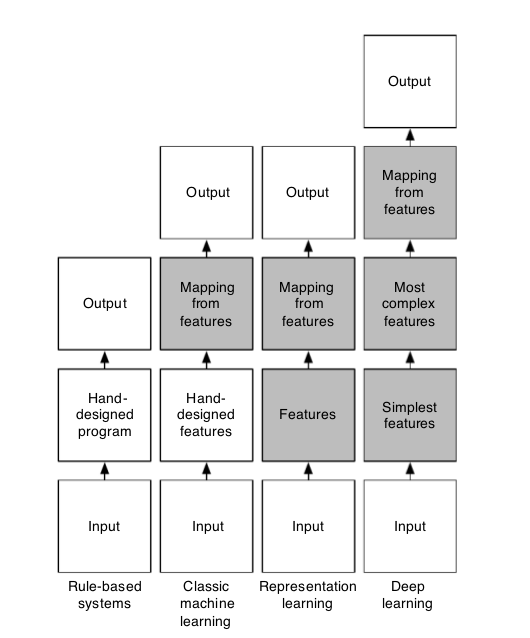
\includegraphics[height=200pt]{diff_between_aprochs.png}
    \caption*{differenze generali tra \\ le diverse tipologie di algoritmi}
  \end{subfigure}
  \label{fig:graph1}
\end{figure}

\subsubsection{Le reti feed-forward (MLP)}

\begin{wrapfigure}{r}{0.4\textwidth}
	\centering
	\vspace{-25pt}
    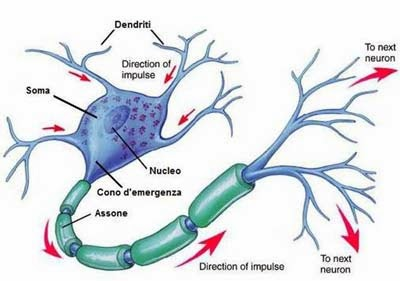
\includegraphics[width=0.4\textwidth]{neurone.jpg}
  	\caption{Il neurone biologico}
  	\label{fig:graph2}
  	\vspace{-20pt}
\end{wrapfigure}

Uno dei modelli della famiglia del deep learning più comuni e semplici da utilizzare sono le reti neurali feed-forward o multi layer perceptron, le quali sono assimilabili a modelli di regressione statistica.\\
Le reti neurali sono un modello matematico molto semplificato del\\ cervello, e per parlarne è necessario qualche riferimento al modello \\biologico.

\subsubsection*{Il neurone biologico}
L'unità base del cervello è rappresentata dai neuroni (Figuara \ref{fig:graph2}),\\ i quali a loro volta sono composti dai dendriti, dal soma, dall'assone e dalle sinapsi. 
\\I dendriti sono l'apparato di input del neurone, attraverso il quale riceve i segnali dall'ambiente o da altri neuroni, tali segnali caricano il neurone, che accumula un potenziale elettrico all'interno del soma.
In determinate condizioni o al raggiungimento di una certa soglia di potenziale il neurone emette un impulso lungo l'assone giungendo alle sinapsi, poste alla fine dell'assone, le quali sono connesse con altri neuroni o con altri apparati del corpo, come i muscoli.\\
Questa particolare cellula oltre a scambiare impulsi è in grado di accumulare informazioni attraverso l'ispessimento o l'assottigliamento della guaina mielinica, la quale è presente lungo l'assone.
Le variazioni dello spessore della guaina comportano un aumento o una diminuzione della resistenza elettrica dell'assone determinando una variazione dell'impulso percepito dai neuroni connessi alle sinapsi a parità di potenziale rilasciato.   

\subsubsection*{Il percettrone} 

\begin{wrapfigure}{r}{0.4\textwidth}
	\centering
	\vspace{-15pt}
    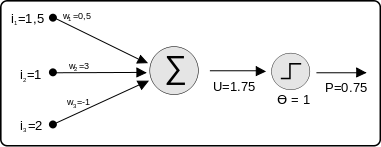
\includegraphics[width=0.4\textwidth]{percettrone.png}
  	\caption{Il percettrone}
  	\label{fig:graph3}
\end{wrapfigure}

Il neurone artificiale è composto da una serie di connessioni in ingresso, come i dendriti nel caso del neurone biologico, questa volta però il compito di immagazzinare informazione viene svolto da queste connessioni in input e non più dalle connessioni in output. 
Ad ogni input del neurone è associato un coefficiente che moltiplica il potenziale in ingresso, a questo punto gli ingressi pesati giungono al nodo sommatore, il corrispettivo del soma, che ne accumula la sommatoria.
Lo step successivo è il blocco contenente la funzione di trasferimento, una funzione che prende in input il potenziale del neurone e rende disponibile il risultato come output finale o come input per i neuroni successivi.
La funzione di trasferimento del neurone può essere di vari tipi, può variare infatti anche tra i neuroni della medesima rete, alcune delle più comuni \\sono:
\begin{wrapfigure}{r}{0.4\textwidth}
	\centering
	\vspace{-120pt}
    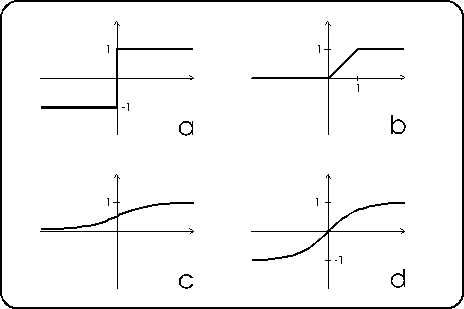
\includegraphics[width=0.4\textwidth]{FDTs.png}
  	\caption{Le funzioni di trasferimento}
  	\label{fig:graph4}
\end{wrapfigure}
(a) la funzione gradino. \\
(b) la funzione lineare con saturazione \\
(c) la funzione sigmoide tra 0 e 1 \\
(d) la funzione sigmoide tra -1 e 1 \\ \\
Volendo esprimere il percettrone in termini matematici si ottiene la seguente \\ equazione:

$\hspace*{100pt} y = f(P) = f(\textstyle\sum_i W_i \cdot X_i)$\\
\(\mathnormal{y}\) - output del percettrone\\
\(\mathnormal{f}\) - funzione di trasferimento del percettrone\\
P - potenziale del neurone\\
\(W_i\) - peso o coefficiente dell'i-esimo ingresso\\
\(X_i\) - potenziale d'ingresso dell'i-esimo neurone\\
\\Una delle caratteristiche più importanti del percettrone è la sua capacità di compiere separazioni lineari. Tali separazioni avvengono in uno spazio a n dimensioni, dove n corrisponde al numero di variabili in ingresso al neurone, perciò si avrà ad esempio per un percettrone a due input la capacita di separare i valori su \(\Re^2\) attraverso un retta, nel caso \(\Re^3\) si potranno separare i valori dello spazio tridimensionale attraverso un piano, e così via.\\
\begin{figure}[h!]
  \centering
  \begin{subfigure}[t]{0.45\linewidth}
  	\centering
  	%\hspace{-120pt}
    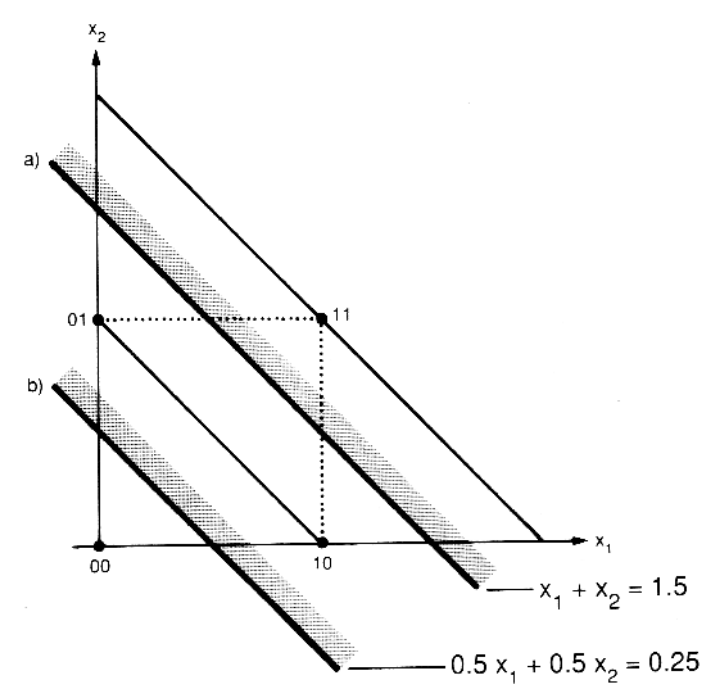
\includegraphics[height=240pt]{sepAndOr.png}
    \captionsetup{justification=centering}
    \caption*{esempio di linee di separazione per neurone a 2 ingressi binari\\
    (a - funzione OR)\\
    (b - funzione AND)}
  \end{subfigure}
  \begin{subfigure}[t]{0.45\linewidth}
    %\hspace{-200pt}
  	\centering
    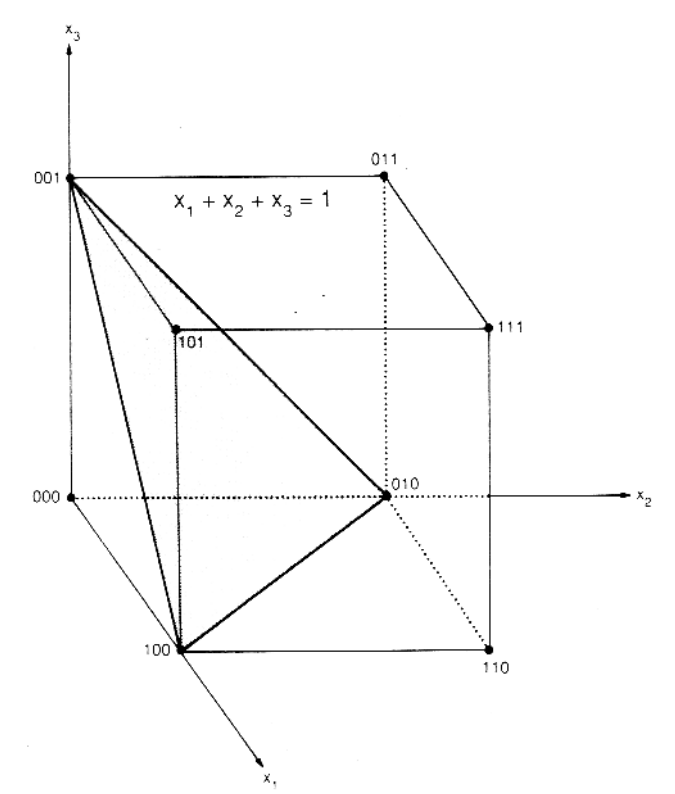
\includegraphics[height=240pt]{sepR3.png}
    \captionsetup{justification=centering}
    \caption*{esempio di piano diseparazione lineare \\ a 3 ingressi per un neurone binario}
  \end{subfigure}
  \label{fig:graph5}
\end{figure}
\\ \\

\subsubsection*{Le reti multi-strato e la separazione non lineare} 
Le reti multi-strato sono composte da strati di percettroni, interconnessi tra loro in modo che gli output degli strati precedenti siano connessi con gli input dei percettroni successivi. Tale struttura "profonda" permette di rappresentare funzioni non linerai molto complesse, tanto più sono gli strati della rete.\\
Uno degli esempi che meglio chiarisce questa problematica è la funzione xor nel seguente esempio, la quale per semplicità è rappresentata con neuroni binari a soglia.

\subsubsection*{Il problema dello XOR}
Lo xor è una delle funzioni non lineari più semplice, nella quale diventa evidente l'impossibilità di approssimare tale funzione con un solo strato di neuroni.
Il grafico illustra come un neurone singolo possa effettuare la separazione lineare che riproduce la funzione and e or, ma come si nota lo xor necessità di due parabole per la separazione e non più di rette, tale separazione si effettua utilizzando una rete ad almeno due strati. 
%
\begin{figure}[h!]
  \centering
  \begin{subfigure}[t]{0.45\linewidth}
  	\centering
  	%\hspace{-120pt}
    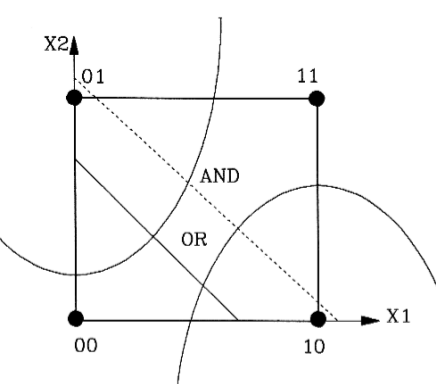
\includegraphics[height=140pt]{SepXor.png}
    \captionsetup{justification=centering}
    \vspace{10pt}
    \caption*{Esempio di linee di separazione per and or e xor}
  \end{subfigure}
  \begin{subfigure}[t]{0.45\linewidth}
    %\hspace{-200pt}
    \vspace{-130pt}
  	\centering
    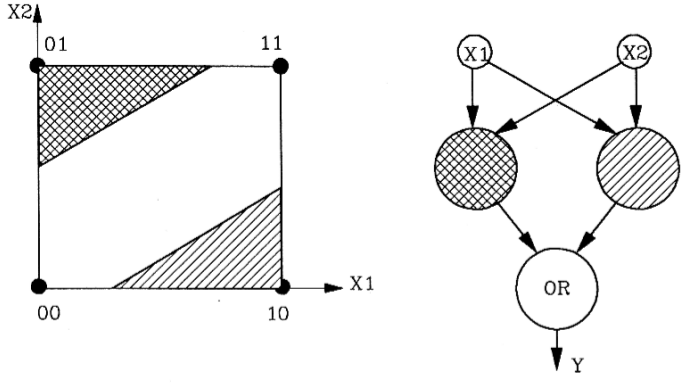
\includegraphics[height=140pt]{MLPxor.png}
    \captionsetup{justification=centering}
    \caption*{MLP in grado di rappresentare la funzione xor}
  \end{subfigure}
  \label{fig:graph6}
\end{figure}
%
\subsubsection{La funzione di addestramento: Il back-propagation} 
Come già detto la struttura della rete neurale deve apprendere una data funzione da dei dati.\\
Tale operazione si effettua presentando degli input alla rete ai quali questa risponderà con degli output, i quali dovranno essere confrontati con degli output corretti per il set di input presentato, per calcolare l'errore nell'output della rete.\\
L'errore che la rete commette ad ogni tentativo viene utilizzato per calcolare attraverso una prescelta funzione, nel nostro caso il BP, dei coefficienti di correzione che vanno applicati ai pesi della rete per avvicinare il suo output a quello desiderato. \\
Come dice il nome "retropropagazione" in italiano, l'errore calcolato dall'output viene applicato ai neuroni precedenti e poi a quelli ancora precedenti fino ad arrivare al primo strato, tale procedura puo essere effettuata in diversi modi, calcolando gli errori su un determinato numero di esempi del dataset, accumulando le correzioni ed applicandole successivamente, tale tecnica è attualmente la più utilizzata ed è detta "mini-batch", ma è possibile anche effettuare la correzione esempio per esempio, e questo è detto addestramento in-line, in fine tra i metodi più comuni c'è anche la possibilità di eseguire tutti gli esempi del dataset e solo alla fine di un'intero ciclo di addestramento applicare le correzioni. questi tre metodi ovviamente risultano validi ma a seconda del problema da risolvere possono avere prestazioni migliori o peggiori in modo difficilmente prevedibile.
\\
Dopo questa introduzione generale all'addestramento delle reti passiamo a dare una vista più accurata dell'algoritmo utilizzato nel progetto che è principalmente pensato per reti mlp con neuroni ad ingressi continui e con funzione di trasferimento sigmoidea o ad arcotangente.
\\
Il BP cerca di minimizzare l'errore quadratico medio, relativo a un training set di esempi dati, scendendo lungo la superficie d'errore e seguendo la direzione di massima pendenza, in cerca di una "valle" sufficientemente profonda. \\
Consideriamo una rete con n input $X_i$ (i = 1, 2,.. n), uno strato nascosto di q neuroni $Z_k$ (k = 1, 2..., q) e uno strato output di m neuroni $Y_j$; (j = 1, 2... m).
Il training set sia costituito da p esempi o casi $C_r$, (r = 1, 2,..,p). Tutti i neuroni abbiano la stessa funzione di trasferimento.\\
L'errore quadratico medio dello strato output è:\\ \\
\begin{equation} \label{eq:eqm}
E = \frac{1}{2} \sum_j{\sum_r{(Y_{rj} - D_{rj})^2}}
\end{equation}

dove Y, è l'output del neurone $Y_j$ alla presentazione dell'esempio $C_r$ e $D_{rj}$ è il
suo valore desiderato. Per semplificare la notazione, eliminiamo l'indice r e minimizziamo l'errore quadratico medio ad ogni presentazione di esempio (modalità on-line), anziché dopo ogni ciclo completo di presentazione del training set
o epoca (modalità batch). Avremo allora:
\\ \\
\begin{equation} \label{eq:eq}
E = \frac{1}{2} \sum_j{(Y_{j} - D_{j})^2}
\end{equation}
\\ \\
Si applica a questo punto la regola del gradiente (fig. Propagazione a):

\begin{equation} 
\label{eq:grad}
\Delta W_{jk} = - \eta \frac{\partial E}{\partial W_{jk}} = - \eta \frac{\partial E}{\partial Y_j} \frac{\partial Y_j}{\partial P_j} \frac{\partial P_j}{\partial W_{jk}} = 
-\eta(Y_j - D_j)f'(P_j)Z_k
\end{equation} \\
\begin{equation} \label{eq:dey}
\frac{\partial E}{\partial Y_j} = (Y_j - D_j)
\end{equation} \\
\begin{equation} \label{eq:dyp}
\frac{\partial Y_j}{\partial P_j} = f'(P_j) 
\end{equation} \\
\begin{equation} \label{eq:dpw}
\frac{\partial P_j}{\partial W_{jk}} = \frac{\partial(\sum W_{jk} Z_k)}{\partial W_{jk}} = Z_k
\end{equation}

Ponendo a questo punto:
\begin{equation} \label{eq:cr}
\delta_j = (Y_j - D_j)f'(P_j) 
\end{equation}
\\
\begin{equation} \label{eq:gradcr}
\Delta W_{jk} = -\eta \ \delta_j \ Z_k
\end{equation}
La formula (\ref{eq:grad}) viene impiegata per aggiornare i pesi sinattici delle connessioni tra strato nascosto e strato output, analogamente, per quanto riguarda le connessioni tra strato input e strato nascosto si utilizza la formula (fig. Propagazione b):
\begin{equation} \label{eq:dih}
\Delta W_{ki} = -\eta \frac{\partial E}{\partial W_{ki}} = - \eta \frac{\partial E}{\partial Z_k} \frac{\partial Z_k}{\partial P_k} \frac{\partial P_k}{\partial W_{ki}} = -\eta \frac{\partial E}{\partial Z_k}f'(P_k)X_i
\end{equation}
Confrontando questa formula con la precedente formula (\ref{eq:grad}), al posto degli errori noti $(Y_j - D_j)$ troviamo le derivate $\frac{\partial E}{\partial Z_k}$, che dobbiamo ora calcolare retropropagando l'errore dallo strato output a ogni neurone nascosto:
\begin{equation} 
\frac{\partial E}{\partial Z_k} = \sum_j \Bigg( \frac{\partial E}{\partial Y_j} \frac{\partial Y_j}{\partial P_j} \frac{\partial P_j}{\partial Z_k} \Bigg) = \sum_j (Y_j - D_j)f'(P_j)W_{jk} 
\end{equation}

o anche, applicando la formula (\ref{eq:cr}) :
\begin{equation}
\frac{\partial E}{\partial Z_k} = \sum_j \ \delta_j \ W_{jk}
\end{equation}
\begin{figure}[h!]
  	\centering
  	%\hspace{-105pt}
    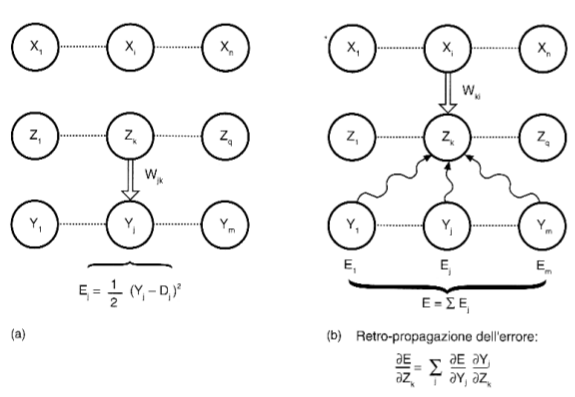
\includegraphics[height=300pt]{PropagationGraph.png}
    \captionsetup{justification=centering}
    \caption*{Propagazione dell'errore nella rete}
  \label{fig:graph7}
\end{figure}
\\
In fine otteniamo le equazioni:
\begin{equation} \label{eq:dih}
\Delta W_{ki} = -\eta f'(P_k)(\sum_j \delta_j W_{jk})X_i
\end{equation}
che ponendo:
\begin{equation} \label{eq:dbpk}
\delta_k = f'(P_k)(\sum_j \delta_j W_{jk})
\end{equation}
la quale assume la stessa forma della (\ref{eq:gradcr}) :
\begin{equation} \label{eq:dpk}
\Delta W_{ki} = -\eta \ \delta_k \ X_i
\end{equation}
Le formule (\ref{eq:dih}) (\ref{eq:dbpk}) (\ref{eq:dpk}) sono valide non solo per aggiornare i pesi sinattici tra strato nascosto (l’unico nella rete che abbiamo ipotizzato) e strato input ma anche, in reti più generali, per le connessioni tra due strati nascosti consecutivi.
Se si adotta la funzione di trasferimento sigmoide si ha:

\begin{equation}
Y = f(P) = \frac{1}{1+e^{kP}}
\end{equation}
\begin{equation}
f'(P) = kf(P)(1-f(P)) = kY(1-Y)
\end{equation}
Dove k è proporzionale alla pendenza della sigmoide nel suo punto di flessione, normalmente si pone k = 1.
A questo punto otteniamo la rielaborazione delle formule (\ref{eq:gradcr}) (\ref{eq:dih}):
\begin{equation}
\Delta W_{jk} = -\eta k (Y_J - D_j)Y_j(1-Y_j)Z_k
\end{equation} 
\begin{equation}
\Delta W_{ki} = -\eta k Z_k (1-Z_k)(\sum_j \delta_j W_{jk})X_i
\end{equation} 
infine i pesi sinattici vengono aggiornati, ad ogni tempo t dell'intervallo 1, 2, ..., (t-1), t, (t+1), ...ecc con:
\begin{equation}
W_{jk}(t+1) = W_{jk}(t) + \Delta W_{jk}
\end{equation}
\begin{equation}
W_{ki}(t+1) = W_{ki}(t) + \Delta W_{ki}
\end{equation} 
\clearpage
\subsection{Il computo parallelo}
L'incremento di prestazioni dei calcolatori fa sempre più affidamento all'ausilio delle GPU, le quali vengono utilizzate sempre di più per operazioni non prettamente grafiche, le quali presentano un' architettura che punta alla massimizzazione del numero di unità di elaborazione e non più all'incremento della frequenza di lavoro.\\
Tale approccio non è sempre il migliore, infatti la loro efficacia è strettamente legata al tipo di applicazioni, in particolare alla parallelizzabilità del codice, ovvero alla dipendenza di determinate istruzioni di avere a disposizione i dati elaborati da istruzioni precedenti.\\
Questa architettura trova la massima efficacia quando un grande numero di istruzioni è completamente indipendente dalle altre. 

\begin{figure}[h!]
  \centering
  \begin{subfigure}[t]{0.45\linewidth}
  	\centering
    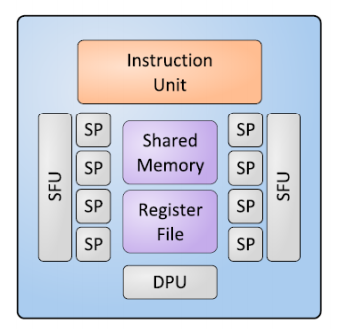
\includegraphics[height=200pt]{SM.PNG}
    \caption*{Struttura di uno stream-multiprocessor}
  \end{subfigure}
  \begin{subfigure}[t]{0.45\linewidth}
  	\centering
    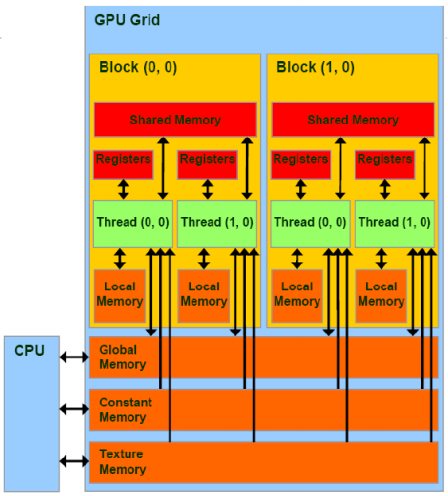
\includegraphics[height=200pt]{LogicModel.PNG}
    \caption*{Struttura logica della GPU}
  \end{subfigure}
  \label{fig:graph1}
\end{figure}

\subsubsection{L'architettura della GPU}
La struttura della GPU è definita "SIMT" (single instruction, multiple thread), tale aggettivo è dato in quanto la GPU è realizzata per eseguire un medesimo programma su un gran numero di processori contemporaneamente, i quali però ricevono dati diversi da computare.\\ Tipicamente i processori presenti su una GPU sono più piccoli e semplici di quelli di una CPU e anche molto meno performanti ma il loro grande numero e la strutturazione delle memorie presenti al suo interno permette per il codice parallelizzabile di ottenere tempi di esecuzione estremamente minori rispetto a quelli in una CPU.\\
Uno dei componenti più importanti in una GPU è lo stream-multiprocessor, Il quale  può essere considerato un processore vettoriale, una GPU solitamente ne contiene diversi, e compongono il modello fisico della GPU, i quali a loro volta sono composti principalmente da tre  unità di calcolo: 

\begin{itemize}
  \item \textbf{SP (scalar processor)} - E' un'unita logica che esegue operazioni in virgola fissa e mobile di un solo thread per volta, è inportante inoltre sapere che gli SP di uno stesso SM hanno una memoria detta shared condivisa che gli permette di scambiarsi dati con estrema velocità a tempo di esecuzione.
  \item \textbf{SFU (special functions unit)} - E' un'unità logica di supporto agli SP che esegue a livello HW funzioni complesse come le funzioni gognometriche e trascendenti che appesantirebbero eccessivamente gli SP.
  \item \textbf{DPU (double proces unit)} - Quest'ultima si occupa delle operazioni su numeri a 64 bit, i double.
\end{itemize}

Una delle peculiarità più importanti della GPU è la differenza tra il modello fisico e quello logico, infatti il modello al quale il programmatore deve far riferimento per ottimizzare l'esecuzione del codice è una via di mezzo tra quello logico e quello che la macchina implementa fisicamente, cercando il bilanciamento migliore possibile tra comprensibilità dei dati e ottimizzazione del codice.
Il modello logico. Il programmatore infatti ha la possibilità di interagire e modellare questa struttura composta da oggetti logici detti griglie (GRID), tali griglie possono avere tre dimensioni e a loro a volta sono composte da altri oggetti logici detti blocchi, i quali possono avere fino a tre dimensioni, che in fine sono composti da thread.
Ogni SM generalmente processa un blocco alla volta, mettendo a disposizione la sua shared memory tra i thread dello stesso blocco, tra i vari blocchi e griglie è possibile lo scambio di informazioni esclusivamente attraverso la global memory, molto più grande delle cache degli SM ma anche molto più lenta. 
Un'ultimo argomento da trattare riguardo il legame tra la struttura logica e quella hardware della GPU è \underline{"il flusso di esecuzione"} ovvero il metodo con cui lo scheduler, ovvero l'organo interno che si occupa della ripartizione delle operazioni ,strutturate dal programmatore nella griglia, ai vari SM. Tale operazione ha come unità base il \underline{warp}, ovvero un numero n dipendente dalla specifica architettura, nel nostro caso 32, di thread appartenenti allo stesso blocco che vengono eseguiti contemporaneamente in maniera "lookstepped" (ovvero in sincronizzazione forzata). L'esecuzione del warp si conclude e si passa al successivo solo nel momento in cui tutti i suoi thread arrivano a fine esecuzione indipendentemente dalla "branch" di programma che hanno seguito.
\\ \\
\subsubsection{L'utilizzo della GPU per il deep-learning}
Nel deep learning come illustrato nella sezione precedente, si effettuano moltissimi calcoli, i quali sono per gran parte scorrelati tra loro, caratteristica questa fondamentale per la parallelizzazione delle operazioni.
L'utilizzo di calcolatori paralleli per l'addestramento delle reti neuronali consente di completare addestramenti per modelli molto grandi in tempi molto ridotti. Confrontando l'addestramento di una rete su una CPU desktop rispetto ad una GPU da gaming si possono incrementare le prestazioni da 200 a 500 volte, ciò significa che un addestramento di un'ora su GPU, può richiedere su una CPU un tempo che può andare da una a tre settimane. \\ \\
(Nel nostro caso da un i5-4670k abbiamo avuto un incremento di prestazioni di 250 volte su una GPU Nvidia gtx760 asus, con un programma che pecca fortemente di ottimizzazione).     



\subsection{Il kinect}

\begin{wrapfigure}{r}{0.2\textwidth}
	\vspace{-10pt}
  	\centering
   	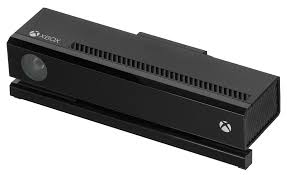
\includegraphics[width=0.2\textwidth]{kinect.jpg}
  	\vspace{-13pt}
  	\caption{Il kinect.}
  	\vspace{-10pt}
\end{wrapfigure}

Il kinect \`e un dispositivo per la rilevazione del movimento, prodotto dall'azienda Microsoft e commercializzato insieme alla console videoludica Xbox. Esso pu\`o tuttavia essere interfacciato ad un comune pc tramite l'apposito connettore. 
Nel kinect \`e presente una fotocamera 1080p RGB, una fotocamera infrarossi per calcolare la profondit\`a e 4 microfoni. Con questo set di sensori ed il suo SDK (software development kit), consente l'utilizzo dei dati prodotti per scopi pi\`u generici, una tra le quali l'utilizzo delle gesture per controllare il pc o la ricostruzione delle espressioni facciali. Questi dati sono resi disponibili attraverso l'apposito SDK e possono essere usati in generici programmi C++, C\# ed altri linguaggi di programmazione, nello specifico per il linguaggio C++ si usa la libreria "Kinect.h".

\subsubsection{Modello dello scheletro}
In particolare ci siamo interessati alla capacit\`a del kinect di poter ricostruire la posizione delle parti del corpo nello spazio, infatti utilizzando la fotocamera infrarossi \`e in grado di rilevare 24 punti diversi nel corpo come indicato in figura \ref{fig:kinmap1}.

\begin{figure}[h]
  	\centering
    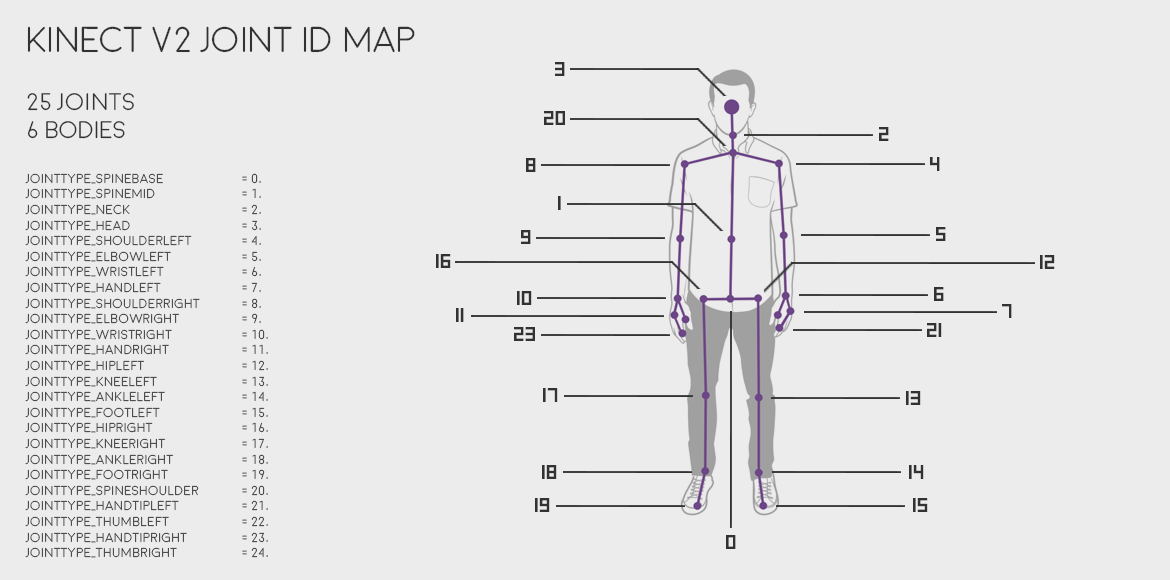
\includegraphics[width=1\textwidth]{kinectskeletonmap.png}
  	\caption{La mappa dei giunti che il kinect \`e in grado di rilevare.}
  	\label{fig:kinmap1}
\end{figure}

\begin{wrapfigure}{r}{0.45\textwidth}
	\vspace{-15pt}
  	\centering
   	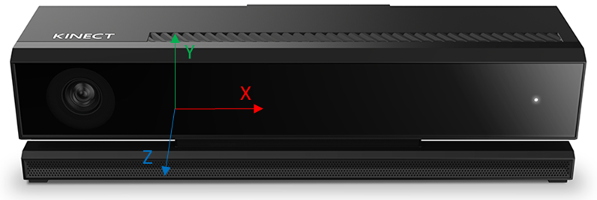
\includegraphics[width=0.45\textwidth]{kin_axis.png}
  	\vspace{-13pt}
  	\caption{Orientazione degli assi rispetto al kinect.}
  	\label{fig:kinaxis1}
  	\vspace{-15pt}
\end{wrapfigure}

I dati di posizione e profondit\`a restituiti dal kinect fanno riferimento alla terna di orientazione indicata in figura \ref{fig:kinaxis1}. Per in nostri scopi abbiamo utilizzato delle procedure gi\`a definite dalla libreria che permettono di acquisire la posizione nello spazio di ogni singolo giunto dello scheletro e il suo stato di tracciamento, se la sua posizione \`e stata interpolata o \`e stato effettivamente tracciato.


\clearpage
\subsection{Scheda enbedded}
Per questo progetto abbiamo realizzato una scheda enbedded che comprendesse l'imu, un modulo bluetooth, la batteria con il suo regolatore e un arduino. 

\begin{figure}[h]
	\centering
	%\vspace{-10pt}
	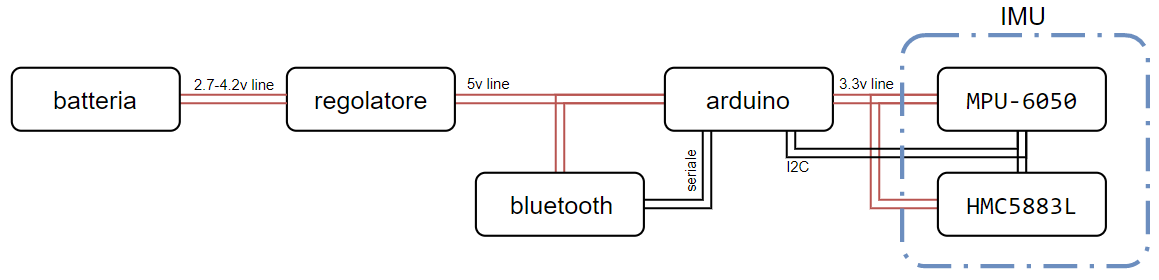
\includegraphics[width=0.80\textwidth]{scheda.png}
	\vspace{-10pt}
	\caption{Schema scheda enbedded}
	\label{fig:schema_scheda}
\end{figure}

\begin{figure}[h]
	\centering
	\vspace{-10pt}
	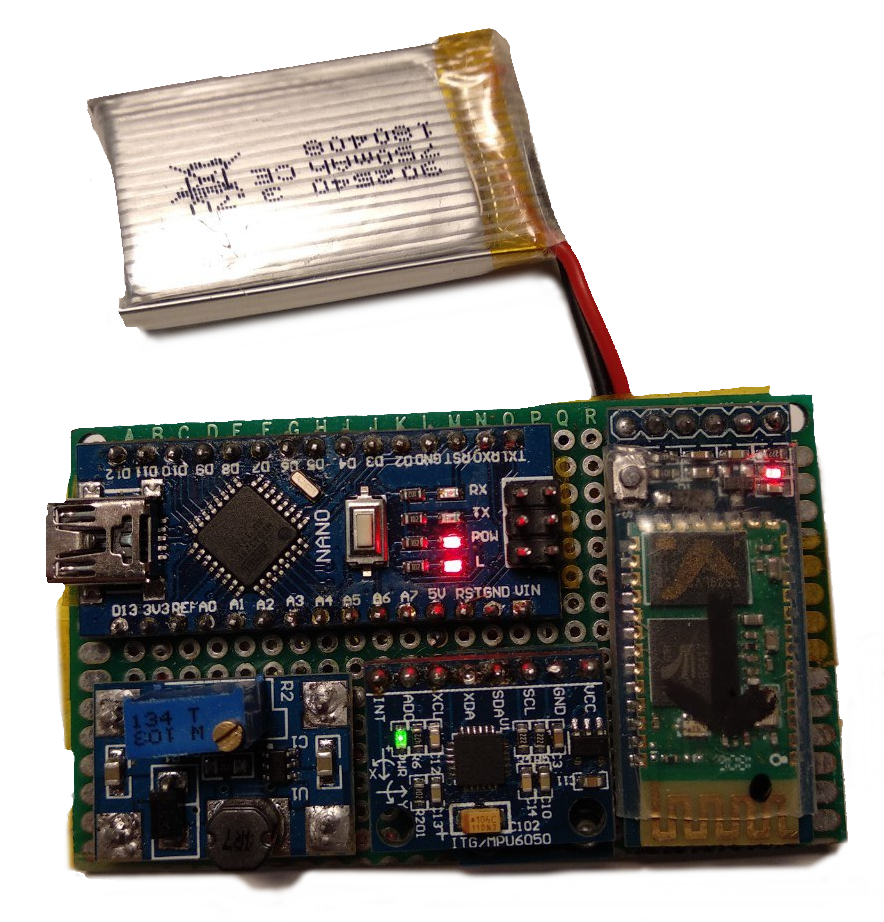
\includegraphics[width=0.50\textwidth]{scheda.jpg}
	\vspace{-10pt}
	\caption{Scheda enbedded}
	\label{fig:scheda}
\end{figure}
La scheda \`e stata realizzata su millefori saldando e wrappando i diversi componenti.
\subsubsection{Arduino}

\begin{wrapfigure}{r}{0.2\textwidth}
	\centering
	\vspace{-30pt}
	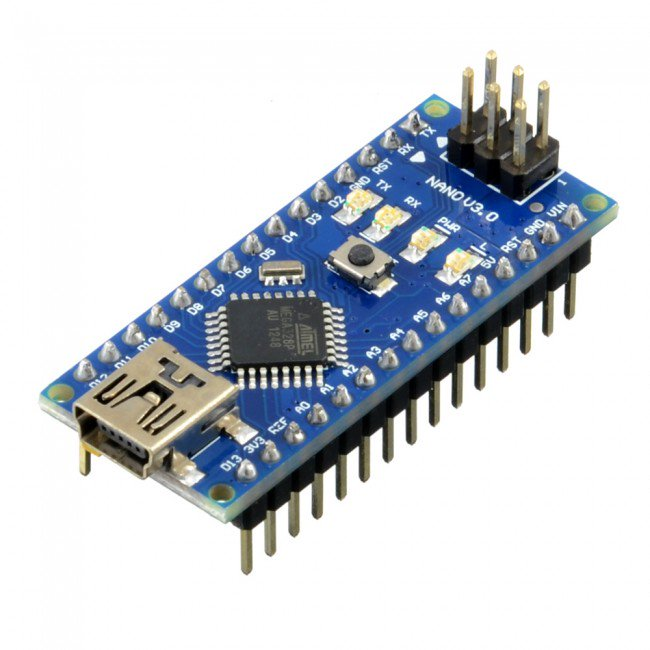
\includegraphics[width=0.2\textwidth]{arduino.jpg}
	\vspace{-30pt}
	\caption{Arduino nano}
	\label{fig:arduino_nano}
	\vspace{0pt}
\end{wrapfigure}

Arduino \`e una piattaforma hardware open-source dotata di microcontrollore e tutto il suo ecosistema, questo lo rendono estremamente utile per realizzare progetti che non richiedono specifiche particolari senza doveresi realizzare una scheda apposita. Le schede arduino possono essere programmate attraveso l'ide proprietario "Arduino IDE", che oltre ad includere la compatibilit\`a con tutte le schede arduino offre alcuni strumenti utili come il motitor seriale.
%
\\
Nel nostro progetto abbiamo usato la scheda "Arduino nano" (fig.\ref{fig:arduino_nano}), si alimenta a \SI{5}{\volt} e include un regolatore di tensione da \SI{5}{\volt} a \SI{3.3}{\volt}, una seriale, l'I2C ed altri pin general purpose.
%
\\
Il regolatore interno \`e stato usato per alimentare i moduli HMC5883L e MPU-6050 che costituiscono l'imu della scheda, la seriale \`e stata utilizzata per comunicare con il modulo bluetooth HC-05, il bus di comunicazione I2C \`e stato usato per interfacciarsi con l'imu ed un pin GPIO \`e stato usato per controllare lo stato del modulo bluetooth.

\subsubsection{Bluetooth}
\begin{wrapfigure}{r}{0.2\textwidth}
	\centering
	\vspace{-30pt}
	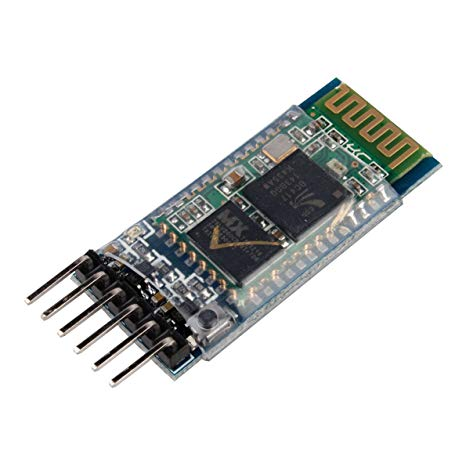
\includegraphics[width=0.2\textwidth]{HC-05.jpg}
	\vspace{-30pt}
	\caption{HC-05}
	\label{fig:HC-05}
	%\vspace{-30pt}
\end{wrapfigure}

Il modulo bluetooth ulilizzato \`e "HC-05", ha 6 pin per interfacciarsi con le atre periferiche: 2 di alimentazione, 2 per la seriale, state e key. 
\\
Questo modulo ha un regolatore da \SI{5}{\volt} a \SI{3.3}{\volt} integrato, quindi va alimentato a \SI{5}{\volt}.
\\
Per comunicare con arduino usa la seriale (RS-232) con livello logico \SI{3.3}{\volt}, ci\`o comporta la necessit\`a di inserire un partitore sul pin rx del modulo (quindi il pin tx di arduino). 
\\
Il pin state e\` stato usato per far conoscere ad arduino quando il modulo ha stabilito la connessione con il computer. 
\\
Il pin key svolge una funzione particolare poich\`e permette di avviare il modulo in modalit\`a "command mode", in questa modalit\`a si possono usare gli AT commands per programmare il modulo (es. cambiare nome al dispositivo, oppure cambiare il baud rate della seriale).
\\
I comandi AT e la loro descrizione si trovano sul datasheet del modulo. 
\\
Per avviare l'HC-05 in modalit\`a AT si deve collegare il modulo all'alimentazione tenendo premuto il pulsante che si trova sulla scheda, dopodiche si pu\`o procedere ad inviare gli at command tramite seriale con un baud rate di 38400Bd. Per fare ci\`o abbiamo collegato la seriale del modulo con 2  pin di arduino con supporto PWM ed abbiamo usato la libreria software serial per poter avere un'altra seriale (la principale connessa al pc e la secondaria connessa al modulo). 
\\
Dopodich\`e basta programmare arduino in modo che reindirizzi ci\`o che gli viene scritto dal pc al modulo, e viceversa. il programma usato \`e il seguente:
%
\begin{lstlisting}[style=myArduino]
#include <SoftwareSerial.h>

SoftwareSerial BTSerial(10, 11); // RX | TX

void setup()
{
  Serial.begin(9600);
  Serial.println("Enter AT commands:");
  BTSerial.begin(38400);  // HC-05 default speed in AT command more
}

void loop()
{
  // Keep reading from HC-05 and send to Arduino Serial Monitor
  if (BTSerial.available())
    Serial.write(BTSerial.read());

  // Keep reading from Arduino Serial Monitor and send to HC-05
  if (Serial.available())
    BTSerial.write(Serial.read());
}
\end{lstlisting}
Cos\`i facendo abbiamo impostato il baud rate a \SI{115200}{\hertz}.

\subsubsection{L'imu}
L'imu (inertial measurement unit) permette di misurare le forze ad esso applicate e l'orientazione dello stesso. Questo viene solitamente fatto combinando i dati di accelerometro, magnetometro e giroscopio. In particolare l'accelerometro misura le accelerazioni, da cui in condizioni di moto inerziale si pu\`o estrarre il vettore gravit\`a sui 3 assi determinando quindi l'angolazione rispetto al suolo; Il magnetometro rileva invece il campo magnetico terrestre su 3 assi, dando cos\`i indicazione della direzione "nord"; Infine il giroscopio restituisce le accelerazioni angolari.
Per questo specifico progetto si sono utilizzati i moduli commerciali "MPU-6050" (fig.\ref{fig:MPU6050}) e "HMC5883L" (fig.\ref{fig:HMC5883L}), rispettivamente come accelerometro pi\`u giroscopio e magnetometro. 

\begin{figure}[h]
    \centering
    \begin{subfigure}[b]{0.3\textwidth}
        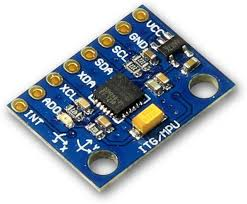
\includegraphics[height=0.75\textwidth]{MPU-6050.jpg}
        \caption{MPU-6050}
        \label{fig:MPU6050}
    \end{subfigure} 
    \begin{subfigure}[b]{0.3\textwidth}
        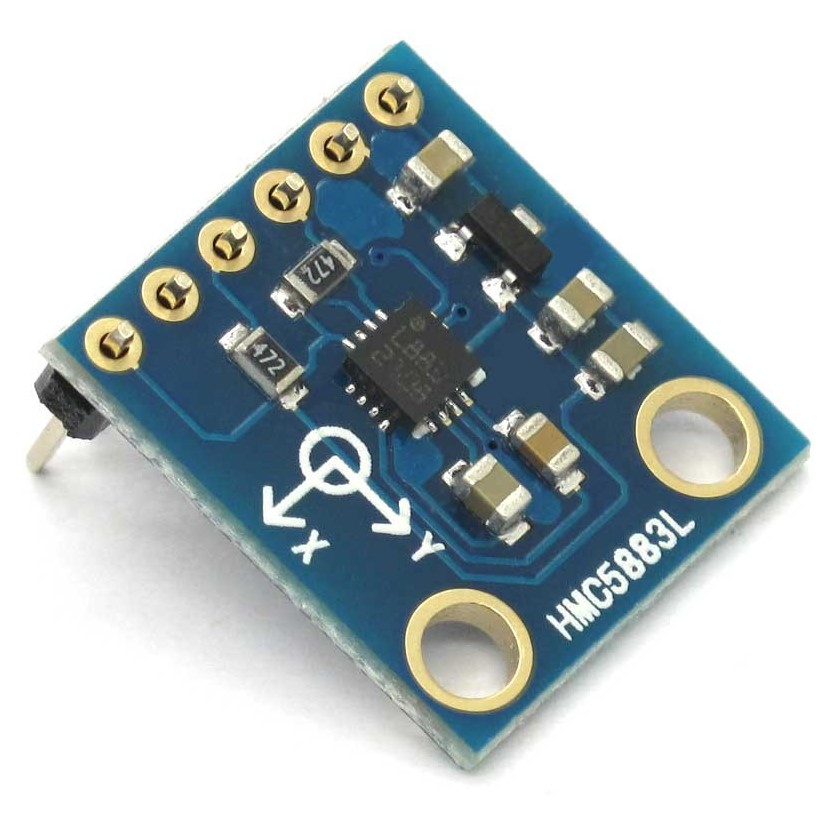
\includegraphics[height=0.75\textwidth]{HMC5883L.jpg}
        \caption{HMC5883L}
        \label{fig:HMC5883L}
    \end{subfigure}
    \caption{l'IMU utilizzata in questo progetto}
    \label{fig:imu}
\end{figure}

Questi dispositivi comunicano con arduino attraverso il protocollo I2C, sono stati quindi connessi ai pin analogici 5 e 4 di arduino.
In particolare l'MPU-6050 integra un accelerometro su 3 assi ed un giroscopio su 3 assi, che vengono convertiti in digitale da 6 ADC a 16 bits. Inoltre pu\`o essere programmato su diverse precisioni, il giroscopio tra \SI[per-mode = symbol]{+-250}{\degree\per\second} e \SI[per-mode = symbol]{+-2000}{\degree\per\second}, l'accelerometro tra \SI[per-mode = symbol]{+-2}{g} e \SI[per-mode = symbol]{+-16}{g}. Questo modulo ha anche un sensore di temperatura che per questo progetto non \`e  stato usato. Supporta l'I2C fino a \SI{400}{\kilo \hertz}.
\clearpage
\subsubsection{Regolatore di tensione}
\begin{wrapfigure}{r}{0.2\textwidth}
	\centering
	\vspace{-30pt}
	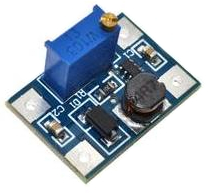
\includegraphics[width=0.2\textwidth]{DC-DC_sx1308.jpg}
	\vspace{-20pt}
	\caption{SX1308}
	\label{fig:sx1308}
	%\vspace{-30pt}
\end{wrapfigure}
\sisetup{range-phrase=-}
Questo regolatore di tensione \`e del tipo switching e permette di elevare la tensione da \SIrange{2}{24}{\volt} a \SIrange{2}{28}{\volt} con un picco massimo di \SI{2}{\ampere}. La tensione di uscita viene impostata girando il trimmer e qualunque sia la tensione in ingresso l'uscita rimarr\`a al valore impostato purch\`e si rispettino i limiti massimi e la tensione di ingresso sia sempre minore di quella di uscita. Nel nostro caso \`e stato molto utile perch\`e la betteria a litio ha una tensione che oscilla tra \SI{2.7}{\volt} quando \`e scarica e \SI{4.2}{\volt} quando \`e carica e questo integrato provvede a stabilizzare l'alimentazione a \SI{5}{\volt}.

\clearpage
\section{Programmi}
\subsection{Overview generale e main server}
Introduciamo i programmi con uno schema generale della relazione logico temporale tra i programmi:
per prima cosa abbiamo dovuto acquisire un dataset ed usarlo per addesrare la rete neurale
\begin{figure}[h]
\centering
\begin{tikzpicture}[node distance=2cm, align=center, every node/.style={fill=white, font=\sffamily}, align=center]
%	\draw[help lines] (-10,-10) grid (1,1);
% ora vanno specificate le posizioni 
%	\node (nome_blocco) 	[tipo_blocco, parentela] 		
%								{testo_blocco};
	\node (prg_ard)			[rect, fill=green!30] 							
								{programma arduino};
	\node (prg_get_data)	[rect, right of=prg_ard, xshift=+4cm, fill=yellow!30] 
								{programma di acquisizione dati};
	\node (file_data_kin)	[round, below of=prg_get_data, xshift=+2.2cm, yshift=-0.75cm, fill=gray!30]	
								{file dati kinect};
	\node (file_data_ard)	[round, below of=prg_get_data, xshift=-2.2cm, yshift=-0.75cm, fill=gray!30]	
								{file dati arduino};
	\node (prg_elab_data)	[rect, below of=prg_get_data, yshift=-3.5cm, fill=yellow!30]
								{programma di post\\ elaborazione dei dati};
	\node (file_dataset)	[round, below of=prg_elab_data, fill=gray!30]	
								{dataset};
	\node (prg_addesr)		[rect, below of=file_dataset, fill=yellow!30]
								{programma di addestramento\\ della rete (OpenLearn)};
	\node (file_pesi_rete)	[round, below of=prg_addesr, fill=gray!30]	
								{modello addestrato};
% per le freccie si fa
%	\daraw[tipo_freccia] (origine) "tipo connessione" "eventuale scritta" (destinazione)			
	\draw[blue, line width=1mm, arrows={[scale=1.75,blue]<->[scale=1.75,blue]}]	
				(prg_ard)		-- 					(prg_get_data);
	\draw[->, red]	(prg_get_data)	to [in=90,out=-90]	(file_data_kin);
	\draw[->, red]	(prg_get_data)	to [in=90,out=-90]	(file_data_ard);
	\draw[->, cyan]	(file_data_kin)	to [in=90,out=-90]	(prg_elab_data);
	\draw[->, cyan]	(file_data_ard)	to [in=90,out=-90] 	(prg_elab_data);
	\draw[->, red]	(prg_elab_data)	-- 					(file_dataset);
	\draw[->, cyan]	(file_dataset)	-- 					(prg_addesr);
	\draw[->, red]	(prg_addesr)	-- 					(file_pesi_rete);
%
\matrix [draw,above] at (current bounding box.south west) {
  \node [shape=circle, fill=green, label=right:programma per la scheda arduino] {}; \\
  \node [shape=circle, fill=yellow, label=right:programma per pc] {}; \\
  \node [shape=circle, fill=gray, label=right:file di testo] {}; \\
  \draw[->, cyan, text=black] ++(-1em, -0em) -- ++(3em, -0em) node[right] {file in input}; \\
  \draw[->, red, text=black] ++(-1em, -0em) -- ++(3em, -0em) node[right] {file in output}; \\
  \draw[blue, text=black, line width=1mm, arrows={[scale=1.75,blue]<->[scale=1.75,blue]}]
  		 ++(-1em, -0em) -- ++(3em, 0) node[right] {in esecuzione contemporanea}; \\
};
\end{tikzpicture}
\caption{i programmi usati per ottenere i pesi della rete addestrata (?)}
\end{figure}
\\
una volta addestrata la rete si possono usare i pesi cos\`i ottenuti per visualizzare in tempo reale il pupo che si muove(???)
\begin{figure}[h]
\centering
\begin{tikzpicture}[node distance=2cm, align=center, every node/.style={fill=white, font=\sffamily}, align=center]
%	\draw[help lines] (-10,-10) grid (1,1);
% ora vanno specificate le posizioni 
%	\node (nome_blocco) 	[tipo_blocco, parentela] 		
%								{testo_blocco};
	\node (prg_ard)			[rect, fill=green!30] 							
								{programma arduino \\ connesso via BT};
	\node (prg_main)	[rect, right of=prg_ard, fill=yellow!30, xshift=4cm] 
								{main socket server: \\ OpenLearn};
	\node (Modello)	[round, above of=prg_main, fill=gray!30]	
								{Modello addestrato};	
	\node (prg_unity)	[rect, right of=prg_main, fill=yellow!30, xshift=4cm]
								{Interfaccia grafica (Unity3D) \\ connesso via socket};
% per le freccie si fa
%	\daraw[tipo_freccia] (origine) "tipo connessione" "eventuale scritta" (destinazione)			
	\draw[blue, line width=1mm, arrows={[scale=1.75,blue]<->[scale=1.75,blue]}]	
					(prg_ard)		-- 	(prg_main);
	\draw[blue, line width=1mm, arrows={[scale=1.75,blue]<->[scale=1.75,blue]}]	
					(prg_main)		-- 	(prg_unity);
	\draw[->, cyan]	(Modello)		--	(prg_main);
\end{tikzpicture}
\caption{una volta addestrata la rete il manichino viene controllato dal suo output in real-time, controllato dai dati ricevuti via BT da arduino. Nella seguente immagine il data-flow va da sinistra verso destra.}
\end{figure}
\\
Il programma principale è stato realizzato in C++, con l'ausilio della libreria boost per l'implementazione dei thread e del server socket, in oltre integra la libreria OpenLearn per il caricamento del modello preaddestrato e il processamento dei dati real-time, in tale programma è presente un thread che si occuppa parallelamente della ricezzione dei dati da arduino, tali dati vengono caricati nel circular buffer il quale è eseguito in un altro thread. I dati contenuti nel circular buffer vengono successivamente presi dal thread che esegue il controllo della rete, la quale elabora i dati che vengono poi immagazzinati e inviati al client unity su richiesta. 
\clearpage

\subsection{Programma arduino}
Questo programma si occupa di acquisire i dati dai sensori attraverso l'I2C, elaborarli e scriverli sulla seriale, in modo che il modulo bluetooth li invii al pc. Il programma si scompone nella classe "MPU0\_6050" che gestisce l'accelerometro, nella classe "QMC5883" che gestisce il magnetometro, nella classe "serial" per gestire la seriale e nelle 2 funzioni standard di arduino "setup" e "loop". Inoltre abbiamo usato la libreria "Wire.h" per l'I2C. \\
Nel "setup" si trova soltanto l'inilizializzazione alla seriale per comunicare con il modulo "HC-05", il baud rate impostato \`e lo stesso che \`e stato settato nel modulo tramite la modalit\`a AT:
\begin{lstlisting}[style=myArduino, caption=funzione "setup", captionpos=b]
void setup() 
{
  Serial.begin(115200);
}
\end{lstlisting}
Nella funzione "loop" si trovano le varie dichiarazioni alle altre classi, un while per aspettare che il modulo "HC-05" sia connesso al pc ed il ciclo infinito che provvede ad acquisire i dati dai sensori e scriverli sulla seriale:
\begin{lstlisting}[style=myArduino, caption=funzione "loop", captionpos=b]
void loop() 
{
  // chiamo i costruttori delle 2 classi che gestiscono i sensori e provvedo al loro settaggio.
  QMC5883 mm;
  MPU_6050 aa;
  aa.setting();

  // accendo un led per il debug  
  digitalWrite(13, HIGH);
  
  // aspetto finchè il pin "state" del modulo "HC-05" non diventa alto
  while (!digitalRead(3))
  {
    delay(10);
  }
  
  // quando il bluetooth è connesso posso procedere ad inizializzare e sincronizzare la seriale
  serial ser; 
  ser.sinc(); 

  // spengo il led
  digitalWrite(13, LOW);
  
  while (true)
  {
    // acquisisco i dati del magnetometro e li normalizzo
    mm.get_data();
    mm.normalize(100);
    
    // acquisisco i dati dell'accelerometro
    aa.get_data();

    // li sposto in degli array
    float acc_xyz[] = {aa.get_AcX(), aa.get_AcY(), aa.get_AcZ()};
    float g_xyz[] = {aa.get_GyX(), aa.get_GyY(), aa.get_GyZ()};
    float magn[] = {mm.getX(), mm.getY(), mm.getZ()};

    // li scrivo sulla seriale in modo che il modulo bluetooth li trasmetta al pc.
    ser.send_data(acc_xyz, g_xyz, magn, aa.get_temp());
  }
}
\end{lstlisting}
Qui sono state usate le classi "MPU\_6050", "QMC5883" e "serial".



Le classi "MPU\_6050" e "QMC5883" si occupano di impostare i registri dei 2 moduli ed inoltre hanno metodi che permettono l'estrazione delle misurazioni da loro effettuate. 

L'impostazione dei moduli \`e stata eseguita facendo riferimento ai rispettivi datasheet. 
\begin{lstlisting}[style=myArduino, caption=classe "MPU\_6050", captionpos=b]
class MPU_6050
{
  public:
    int16_t AcX,AcY,AcZ,Tmp,GyX,GyY,GyZ;
    float normalized_AcX, normalized_AcY, normalized_AcZ, normalized_GyX, normalized_GyY, normalized_GyZ;
    float rescaled_AcX, rescaled_AcY, rescaled_AcZ, rescaled_GyX, rescaled_GyY, rescaled_GyZ;
  
    const uint8_t MPU = 0x68; // I2C address of the MPU-6050
    
    // costruttore della classe, accende l'MPU_6050
    MPU_6050(){...}
  
    // prede i dati dall'MPU_6050 e le sposta sulle variabili di classe.
    void get_data(){...}
  
    // funzioni per ritornare i valori dell'accelerometro
    float get_AcX(){ return (AcX*1.0); }
    float get_AcY(){...}
    float get_AcZ(){...}
  
    // funzioni per ritornare i valori del giroscopio
    float get_GyX(){ return (GyX*1.0); }
    float get_GyY(){...}
    float get_GyZ(){...}
    
    // funzioni per ritornare i valori normalizzati dell'accelerometro
    float get_normalized_AcX(){ return normalized_AcX; }
    float get_normalized_AcY(){...}
    float get_normalized_AcZ(){...}
  
    // funzioni per ritornar i valori normalizzati del giroscopio
    float get_normalized_GyX(){ return normalized_GyX; }
    float get_normalized_GyY(){...}
    float get_normalized_GyZ(){...}
  
    // funzioni per calcolare e ritornare la norma dell'accelerometro o del magnetometro
    float norma(float x, float y, float z){...}
    float get_norma_Gy(){ return norma(GyX, GyY, GyZ); }
    float get_norma_Ac(){...}
  
    // funzione per ritornare la temperatura
    float get_temp(){ return Tmp; }
  
    // funzioni per normalizzare l'accelerometro o il magnetometro
    void normalize_Ac(int Max){...}
    void normalize_Gy(int Max){...}
    
    // funzione che scrive le impostazioni all'MPU_6050
    void setting(){...}
};
\end{lstlisting}

La seguente è la classe di gestione della bussola 3D
\begin{lstlisting}[style=myArduino, caption=classe "QMC5883", captionpos=b]
class QMC5883
{
  public:
    uint8_t add = 0x0D;
    int nowX = 0;
    int nowY = 0;
    int nowZ = 0;
    float rescaled_x = 0; 
    float rescaled_y = 0;
    float rescaled_z = 0;
    
    // il costruttore provvede ad inizializzare il modulo e settarne i vari registri 
    QMC5883(){...}
    
    // funzioni per ritornare i valori x-y-z del magnetometro
    float getX(){ return (nowX*1.0); }
    float getY(){...}
    float getZ(){...}

    // funzioni per ritornare i valori del magnetometro dopo averli riscalati
    float getX_rescaled(){ return rescaled_x; }
    float getY_rescaled(){...}
    float getZ_rescaled(){...}
  
    // funzione che provvede a leggere i regisrti del modulo per acquisire i dati
    // spostandoli nelle variabili di classe
    void get_data(){...}

    // funzioni per calcolare la norma e ritornare i valori normalizzati 
    float norma(float x, float y, float z){...}
    float get_norma(){ return norma(nowX, nowY, nowZ); }
    void normalize(int Max){...}
};
\end{lstlisting}
%
%
Infine la classe serial si occupa di scomporre i dati di tipo float restituiti dai moduli in array di 4 byte che poi vengono trasmessi al modulo bluetooth tramite la seriale.
\begin{lstlisting}[style=myArduino, caption=classe "serial", captionpos=b]
class serial
{
  public:

    // funzione che permette di sincronizzarsi con il pc
    void sinc(){...}

    // union per poter scompattare un float in 4 byte
    union Scomp_float{...};

    // funzione che permette di inviare un intero float scompattandolo in 
    // 4 byte che vengono trasmessi serialmente
    void send_float(float n){...}

    // funzione che permette di riceve un float come sopra
    float receive_float(){...}

    // funzione per l'invio di un solo carattere
    void send_char(char ch){...}

    // funzione per la ricezione di un singolo carattere
    char receive_char(){...}

    // funzione che provvede ad inviare i dati necessari.
    void send_data(float* acc_xyz, float* g_xyz, float* magn, float temp){...} 
};
\end{lstlisting}
Per effettuare l'operazione di serializaziopne dei float in array di byte abbiamo fatto ricorso all'uso di una struttura dati chiamata "union":
\begin{lstlisting}[style=myArduino, caption=classe "serial", captionpos=b]
union Scomp_float
{
  float f;
  int i;
  unsigned char byte_s[4];
};
\end{lstlisting}
Questa struttura dati ha la particolarit\`a che a differenza di una struct, in cui i dati sono memorizzati in modo contiguo nella memoria, l'union memorizza tutti i dati della struttura nelle stesse locazioni di memoria.

\clearpage

\newsavebox{\mylistingboxstruct}
\newsavebox{\mylistingboxunion}

\newsavebox{\mytikzboxonestruct}
\newsavebox{\mytikzboxtwounion}

\begin{figure}[h]
	\centering
	\begin{lrbox}{\mylistingboxstruct}%
		\begin{minipage}{.30\linewidth}%
			\centering
			\begin{lstlisting}[style=mycpp]
struct es_struct
{
  int a;
  unsigned char b[4];
}
			\end{lstlisting}%
		\end{minipage}%
	\end{lrbox}%
	
	
	\begin{lrbox}{\mylistingboxunion}%
		\begin{minipage}{.30\linewidth}%
			\centering
			\begin{lstlisting}[style=mycpp]
union es_union
{
  int a;
  unsigned char b[4];
}
			\end{lstlisting}%
		\end{minipage}%
	\end{lrbox}%
	
	\begin{lrbox}{\mytikzboxonestruct}%
		\begin{minipage}{.50\linewidth}%
			\centering
			\hspace{-1cm}
			\begin{tikzpicture}[every node/.style={rectpile}]
			\node at (0, 0) (A) {0x00};
	        \node [anchor=north] at (A.south) (B) {0x01};
	        \node [anchor=north] at (B.south) (C) {0x02};
	        \node [anchor=north] at (C.south) (D) {0x03};
	        \node [anchor=north] at (D.south) (E) {0x04};
	        \node [anchor=north] at (E.south) (F) {0x05};
	        \node [anchor=north] at (F.south) (G) {0x06};
	        \node [anchor=north] at (G.south) (H) {0x07};
	        
	        \node [anchor=west, draw=black] at (A.east) (M) {};
	        \node [anchor=west, draw=black] at (B.east) (N) {};
	        \node [anchor=west, draw=black] at (C.east) (O) {};
	        \node [anchor=west, draw=black] at (D.east) (P) {};
	        \node [anchor=west, draw=black] at (E.east) (Q) {};
	        \node [anchor=west, draw=black] at (F.east) (R) {};
	        \node [anchor=west, draw=black] at (G.east) (S) {};
	        \node [anchor=west, draw=black] at (H.east) (T) {};
	        
	        \draw [decorate,decoration={brace,amplitude=10pt,raise=0pt},
	            yshift=-0pt,xshift=-0.5cm]
                (2cm,0.25cm) -- (2cm, -1.75cm) node [black,midway,xshift=0.8cm] {\hspace{-8pt}a};
            \draw [decorate,decoration={brace,amplitude=10pt,raise=0pt},
	            yshift=-0pt,xshift=-0.5cm]
                (2cm,-1.75cm) -- (2cm, -3.75) node [black,midway,xshift=0.8cm] {b[ ]};
			\end{tikzpicture}%
		\end{minipage}%
	\end{lrbox}%
	
	
	\begin{lrbox}{\mytikzboxtwounion}%
		\begin{minipage}{.50\linewidth}%
			\centering
			\begin{tikzpicture}[every node/.style={rectpile}]
			\node at (0, 0) (A) {0x00};
	        \node [anchor=north] at (A.south) (B) {0x01};
	        \node [anchor=north] at (B.south) (C) {0x02};
	        \node [anchor=north] at (C.south) (D) {0x03};
	        \node [anchor=north] at (D.south) (E) {0x04};
	        \node [anchor=north] at (E.south) (F) {0x05};
	        \node [anchor=north] at (F.south) (G) {0x06};
	        \node [anchor=north] at (G.south) (H) {0x07};
	        
	        \node [anchor=west, draw=black] at (A.east) (M) {};
	        \node [anchor=west, draw=black] at (B.east) (N) {};
	        \node [anchor=west, draw=black] at (C.east) (O) {};
	        \node [anchor=west, draw=black] at (D.east) (P) {};
	        \node [anchor=west, draw=black] at (E.east) (Q) {};
	        \node [anchor=west, draw=black] at (F.east) (R) {};
	        \node [anchor=west, draw=black] at (G.east) (S) {};
	        \node [anchor=west, draw=black] at (H.east) (T) {};
	        
	        \node [draw=black] at (3, 0) (M1) {};
	        \node [anchor=north, draw=black] at (M1.south) (N1) {};
	        \node [anchor=north, draw=black] at (N1.south) (O1) {};
	        \node [anchor=north, draw=black] at (O1.south) (P1) {};
	        \node [anchor=north, draw=black] at (P1.south) (Q1) {};
	        \node [anchor=north, draw=black] at (Q1.south) (R1) {};
	        \node [anchor=north, draw=black] at (R1.south) (S1) {};
	        \node [anchor=north, draw=black] at (S1.south) (T1) {};
	        
	        \draw [decorate,decoration={brace,amplitude=10pt,raise=0pt},
	            yshift=-0pt,xshift=-0.5cm]
                (2cm,0.25cm) -- (2cm, -1.75cm) node [black,midway,xshift=0.8cm] 
                {\hspace{-10pt}a};
            \draw [decorate,decoration={brace,amplitude=10pt,raise=0pt},
	            yshift=-0pt,xshift=-0.5cm]
                (4cm,0.25cm) -- (4cm, -1.75) node [black,midway,xshift=0.8cm] {b[ ]};

            \draw [densely dotted] (1.5,0.25) -- (3,0.25);              
            
            \draw [densely dotted] (1.5,-1.75) -- (3,-1.75);       
            
			\end{tikzpicture}%
		\end{minipage}%
	\end{lrbox}%
	
	\begin{tabular}{@{}cc@{}}
		%
		\begin{tabular}{@{}c@{}}
		
			\begin{subfigure}[b]{.40\textwidth}
				\centering
				\usebox{\mylistingboxstruct}
				\vspace{-10pt}
				\caption{Struct generico}
	  			\label{fig:es_struct}
	  			\vspace{10pt}
	 		\end{subfigure} \\
	 		
	 		\begin{subfigure}[b]{.45\textwidth}
				\centering
				\usebox{\mytikzboxonestruct}
				\vspace{0pt}
				\caption{Rappresentazione dei dati dello struct\\memorizzati in ram}
	  			\label{fig:struct_ram}
	  			\vspace{0pt}
	 		\end{subfigure}  
			%
			
		\end{tabular}

		\hspace{-50pt}		
		
		\begin{tabular}{@{}c@{}}
			
			\begin{subfigure}[b]{.40\textwidth}
				\centering
				\usebox{\mylistingboxunion}
				\vspace{-10pt}
				\caption{Union generico}
	  			\label{fig:struct_ram}
	  			\vspace{10pt}
	 		\end{subfigure} \\
			
			
			\begin{subfigure}[b]{.45\textwidth}
				\centering
				\usebox{\mytikzboxtwounion}
				\vspace{0pt}
				\caption{Rappresentazione dei dati dell'union\\memorizzati in ram}
	  			\label{fig:es_union}
	  			\vspace{0pt}
	 		\end{subfigure} 
	 		
		\end{tabular}
		
	\end{tabular}
	
	\caption{Confronto tra struct ed union}
	\label{fig:struct_union}
\end{figure}
Come si pu\`o vedere dalla figura \ref{fig:struct_union} lo struct (figura \ref{fig:es_struct}) memorizza i dati in ram facendo partire l'intero dall'indirizzo 0x00 e l'array di byte dall'indirizzo 0x04 (figura \ref{fig:struct_ram}), mentre l'union (figura \ref{fig:es_union}) sovrappone i 2 dati nelle stesse locazioni di memoria (figura \ref{fig:struct_union}).
Cio\`o permmette ad esempio di leggere un intero (o un qualunque altro tipo di dato) come un insieme di byte: con riferimento alla figura \ref{fig:es_union} se pongo:
\begin{lstlisting}[style=myArduino, caption=classe "serial", captionpos=b, label={lst:es_union}]
es_union U;
U.a = 0x0514FFAA;
\end{lstlisting}
e successivamente vado a vedere il valore di b[ ] ottengo i valori:
\begin{lstlisting}[style=myoutput, caption=classe "serial", captionpos=b, label={lst:es_union}]
U.b[0] -> 0x05
U.b[1] -> 0x14
U.b[2] -> 0xFF
U.b[3] -> 0xAA
\end{lstlisting}
che sono esattamente i byte costituenti U.a. Ci\`o ci ha permesso di inviare un float come sequenza di byte al pc, nella classe serial sul pc c'e` esattamente lo stesso tipo di struttura per ricostruire il float. 

\subsection{programma per l'acquisizione dei dati dal kinect e da arduino}
Questo programma \`e stato usato per acquisire i dati da arduino e dal kinect e scriverli in dei file di testo, ce vengono successivamente elaborati. 
%
%
\subsubsection{librerie usate}
La lista completa delle librerie usate \`e:
\begin{lstlisting}[style=mycpp, caption=librerie usate, captionpos=b]
// libreria usata da visual studio, da togliere in caso si usi un altro ide
#include "pch.h"

// librerie standard per i file stringhe e altro
#include <cstddef>
#include <cstdlib>
#include <fstream>
#include <iomanip>
#include <iostream>
#include <ostream>
#include <string>
#include <math.h>

// librerie create da noi
#include "real_time.h"
#include "kin_file_manager.h"
#include "ard_file_manager.h"
#include "data_structure.h"

// libreria per usare i thread
#include <boost/thread.hpp>

// altre librerie per log, alcuni tipi di dato, un buffer FIFO
#include <boost/log/core.hpp>
#include <boost/call_traits.hpp>
#include <boost/circular_buffer.hpp>
#include <boost/container/vector.hpp>

// altre librerie per il logger
#include <boost/log/attributes.hpp>
#include <boost/log/attributes/scoped_attribute.hpp>
#include <boost/log/expressions.hpp>
#include <boost/log/sinks/sync_frontend.hpp>
#include <boost/log/sinks/text_ostream_backend.hpp>
#include <boost/log/sources/basic_logger.hpp>
#include <boost/log/sources/record_ostream.hpp>
#include <boost/log/sources/severity_logger.hpp>
#include <boost/log/utility/setup/common_attributes.hpp>
#include <boost/log/utility/setup/console.hpp>
#include <boost/log/utility/setup/file.hpp>

#include <boost/smart_ptr/make_shared_object.hpp>
#include <boost/smart_ptr/shared_ptr.hpp>

// altre librerie per i thread 
#include <boost/thread/condition_variable.hpp>
#include <boost/thread/mutex.hpp>
#include <boost/thread/thread.hpp>

// librereria per il tempo
#include <boost/date_time/posix_time/posix_time.hpp>

// libreria fatta da noi per gestire la seriale
#include "Serial_handler.h"

// librerie di Windows e kinect 
#include <Windows.h>
#include <Kinect.h>
#include <Shlobj.h>

// namespace standard
using namespace std;
\end{lstlisting}
%
%
\subsubsection{Librerie custom}
Per alleggerire il file "main" abbiamo spostato delle classi in file esterni, che sono a tutti gli effetti delle librerie a se stanti. Abbiamo costruito librerie per: la gestione del tempo, i file manager, le strutture dati e la gestione della seriale.
%
%
\paragraph{Libreria per misurare il tempo}
In "real\_time.h" ci sono alcune funzioni per prendere il tempo e misurarlo:
\begin{lstlisting}[style=mycpp, caption=librerie usate, captionpos=b]
#pragma once

#ifndef _REAL_TIME_H_
#define _REAL_TIME_H_

#include <boost/chrono.hpp>
#include <boost/timer/timer.hpp>

class real_time
{
private:
  boost::timer::cpu_timer timer;
  boost::timer::cpu_times t;

public:
  /// <summary>
  /// start the time counting
  /// </summary>
  /// <returns></returns>
  void start();

  /// <summary>
  /// return enlapsed time in millisecond
  /// </summary>
  /// <returns></returns>
  float stop();

  /// <summary>
  /// get the time in millisecond
  /// </summary>
  /// <returns></returns>
  uint64_t get_curr_time();

};

#endif // #ifndef _REAL_TIME_H_
\end{lstlisting}
%
%
\paragraph{File manager per il kinect}\label{par:kin_file_mng}
In "kin\_file\_manager.h" ci sono le funzioni per gestire il file di testo relativo al kinect:
\begin{lstlisting}[style=mycpp, caption=librerie usate, captionpos=b]
#pragma once

#ifndef _KIN_FILE_MANAGER_H_
#define _KIN_FILE_MANAGER_H_

#include <iostream>
#include <ostream>
#include <fstream>
#include <string>

// in questa libreria sono dichiarate le varie strutture dati
#include "data_structure.h"

class kin_file_manager
{
private:
  std::fstream f;
  std::ios::_Openmode mode;
  unsigned long int line_id = 0;

public:
  // il costruttore provvede a settare il nome del file e la modalit\`a di apertura
  kin_file_manager(std::string file_name, std::ios::_Openmode mode);

  // questa funzione provvede a scrivere un singolo blocco di dati nel file
  void write_data_line(kinect_data dat);

  // funzione che legge un blocco di dati dal file e lo sposta nella struttura dati
  // se si \`e raggiunta la fine del file la funzione ritorna 0, altrimenti ritorna 1. 
  bool read_data_line(kinect_data* dat);

  // distruttore della classe, chiude il file
  ~kin_file_manager()
  {
  f.close();
  }

  // funzione che chiude il file
  void close()
  {
  f.close();
  }

};

#endif // #ifndef _KIN_FILE_MANAGER_H_
\end{lstlisting}
%
%
\paragraph{File manager per arduino}
La libreria "ard\_file\_manager.h" che contiene le funzioni per la gestione del file di testo relativo ai dati di arduino:
\begin{lstlisting}[style=mycpp, caption=librerie usate, captionpos=b]
#pragma once

#ifndef _ARD_FILE_MANAGER_
#define _ARD_FILE_MANAGER_

#include <iostream>
#include <ostream>
#include <fstream>
#include <string>
#include "data_structure.h"


class ard_file_manager
{
private:
  std::fstream f;
  std::ios::_Openmode mode;
  unsigned long int line_id = 0;

public:
  ard_file_manager(std::string file_name, std::ios::_Openmode mode);

  void write_data_line(arduino_data dat);

  bool read_data_line(arduino_data* dat);

  ~ard_file_manager()
  {
    f.close();
  }

  void close()
  {
    f.close();
  }
};

#endif //#ifndef _ARD_FILE_MANAGER_
\end{lstlisting}
Questa libreria \`e strutturata in modo totalmente simile a quella per la gestione dei file del kinect trattata nel paragrafo \ref{par:kin_file_mng} con l'unica differenza che la struttura dati utilizzata \`e relativa ad arduino e non al kinect.
\\
%
%
\paragraph{strutture dati}
La libreria "data\_structure.h" \`e fondamentale e definisce le strutture dati utilizzate nel resto del programma:
\begin{lstlisting}[style=mycpp, caption=librerie usate, captionpos=b]
#pragma once


#ifndef _DATA_STRUCTURE_H_
#define _DATA_STRUCTURE_H_

#include <iostream>
#include <string>
#include <boost/array.hpp>

// struttura dati per gestire i dati provenienti dal kinect
struct kinect_data
{
  static const int number_of_joints = 3;

  // sottostruttura che contiene i dati di ogni giunto: il suo numero, il giunto attaccato ad esso, la posizione e l'angolo rispetto all'altro giunto
  struct joit_data
  {
    int joint_name = -1;
    int to_joint = -1;
    float position[3] = { 0, 0, 0 };
    float angle[3] = { 0, 0, 0 };
  };

  //Tabelle ad accesso diretto utilizzate per ottimizzare la procedura di estrazione dati dalla
  //classe kinect_class e la conversione dai punti nello spazio dello scheletro ad angoli 
  //del braccio. 
  int needed_joint[number_of_joints] = { 8, 9, 10 };
  int to_joint[24] = { -1, -1, -1, -1, -1, -1, -1, -1, 9, 10, -1, -1, -1, -1, -1, -1, -1, -1, -1, -1, -1, -1, -1, -1 };
  int to_ref_joint[24] = { -1, -1, -1, -1, -1, -1, -1, -1, 0, 1, 2, -1, -1, -1, -1, -1, -1, -1, -1, -1, -1, -1, -1, -1 }; // tabella di accesso (chiave numero joint kinect) -> (restituisce l-indice del numero del giunto in needed_joint)    
  float ref_Ang_x[number_of_joints] = { 0, 0, 0 }; //per  8, 9
  float ref_Ang_y[number_of_joints] = { 0, 0, 0 }; //per 8, 9
  float ref_Ang_z[number_of_joints] = { 180, 180, 0 }; //per 8, 9
  float mul_fctor_x[number_of_joints] = { 0, 0, 0 }; //per 8, 9
  float mul_fctor_y[number_of_joints] = { 1, 1, 0 }; //per 8, 9
  float mul_fctor_z[number_of_joints] = { 1, 1, 0 }; //per 8, 9

  joit_data needed_joints[number_of_joints];

  // tempo esatto in cui i dati sono stati acquisiti
  uint64_t frame_time = 0;

  // contatore usato nella post elaborazione dei dati
  uint64_t contatore = 0;

  // funzione per verificare se il frame acquisito \`e parziale o completo 
  bool full_frame();

  // funzione per stampare i dati memorizzati
  void print_data();

  float jointAngleX(float *P1, float *P2);

  float jointAngleY(float *P1, float *P2);

  float jointAngleZ(float *P1, float *P2);

  void updateAngles();

  // funzione per convertire il numero del giunto in una stringa
  std::string joint_Enum_ToStr(int n, std::string language);
};

// struttura dati per gestire i dati provenienti da arduino
struct arduino_data
{
  // variabili che rappresentano i dati: dell'accelerometro, del giroscopio, del magnetometro e la temperatura
  float acc_xyz[3];
  float gy_xyz[3];
  float magn_xyz[3];
  float temp;

  // tempo esatto di acquisizione dei dati
  uint64_t frame_time = 0;

  // ?
  uint64_t contatore = 0;

  // funzione che permette di stampare il set di dati attualmente immagazzinato a schermo 
  void print_data();
};

// struttura template che gestisce un set di dati del dataset
template<typename type_in, std::size_t N, typename type_out, std::size_t M>
struct dataset_data
{
  boost::array<type_in, N> in;
  boost::array<type_out, M> out;

  // stamapa i dati attualmente immagazzinati
  void print_data();
};

#endif //#ifndef _DATA_STRUCTURE_H_
\end{lstlisting}
%
%
\paragraph{Gestione seriale}
Infine, l'ultima libreria fatta da noi ospita la classe che gestisce la seriale per la comunicazione tramite bluetooth con arduino:
\begin{lstlisting}[style=mycpp, caption=librerie usate, captionpos=b]
#pragma once

#ifndef _SERIAL_HADLER_H_
#define _SERIAL_HADLER_H_

#include <iostream>
#include <string>
#include <boost/asio.hpp> 
#include <boost/bind.hpp>
#include <boost/asio/serial_port.hpp> 


class Serial
{
private:
  // dichiaro la porta seriale che verra inizializzata nel costruttore
  boost::asio::serial_port* port;

  // per ricomporre i float ricevuti uso un union
  union Scomp_float
  {
    float n_float;
    uint32_t n_int;
    uint8_t n_bytes[4];
  };

public:
  // nel costruttore si inizializza la seriale e si effettua la connessione al dispositivo bluetooth
  Serial(std::string com);
  
  // effettua una sincronizzazione iniziale tra arduino ed il pc
  void sinc();

  // riceve un float da arduino
  float receive_float();

  // metodo per inviare un carattere
  void send_char(char ch);

  // metodo per ricevere un carattere
  char receive_char();


  // riceve i dati di acc, gy, magn da arduino
  // il metodo ritorna 
  //     -> 0 se la trasmissione \`e andata a buon fine
  //     -> 1 se \`e fallita
  int receive_data(float* acc_xyz, float* g_xyz, float* magn, float* temp);

  ~Serial()
  {
    port->close();
  }
};

#endif // #ifndef _SERIAL_HADLER_H_
\end{lstlisting}
Per trasmettere il blocco di dati da arduino al pc abbiabo sviluppato un "protocollo" di comunicazione, cio\`e i vari dati sono separati da sei tag di controllo che permettono di verificare se il dato \`e stato trasmesso correttamente o no.

\newsavebox{\mylistingboxcodeard}
\newsavebox{\mylistingboxcodepc}
\begin{figure}[h!]
	\centering
	\begin{lrbox}{\mylistingboxcodeard}%
		\begin{minipage}{.40\linewidth}%
			\centering
			\begin{lstlisting}[style=mycpp]
void send_data(float* acc_xyz, float* g_xyz, float* magn, float temp)
{
  send_char('a');
  for (int i = 0; i < 3; i++)
    send_float(acc_xyz[i]);
  send_char('g');
  for (int i = 0; i < 3; i++)
    send_float(g_xyz[i]);
  send_char('m');
  for (int i = 0; i < 3; i++)
    send_float(magn[i]);
  send_char('t');
  send_float(temp);
  send_char(4);
}
			\end{lstlisting}%
		\end{minipage}%
	\end{lrbox}%
	
	
	\begin{lrbox}{\mylistingboxcodepc}%
		\begin{minipage}{.40\linewidth}%
			\centering
			\begin{lstlisting}[style=mycpp]
int Serial::receive_data(float* acc_xyz, float* g_xyz, float* magn, float* temp)
{
  if (receive_char() != 'a')
    return 1;
  for (int i = 0; i < 3; i++)
    acc_xyz[i] = receive_float();
  if (receive_char() != 'g')
    return 1;
  for (int i = 0; i < 3; i++)
    g_xyz[i] = receive_float();
  if (receive_char() != 'm')
    return 1;
  for (int i = 0; i < 3; i++)
    magn[i] = receive_float();
  if (receive_char() != 't')
    return 1;
  temp[0] = receive_float();
  if (receive_char() != 4)
    return 1;
  return 0;
}
			\end{lstlisting}%
		\end{minipage}%
	\end{lrbox}%
	
	
	\begin{tabular}{@{}cc@{}}
		
		
		\begin{subfigure}[b]{.40\textwidth}
			\centering
			\usebox{\mylistingboxcodeard}
			\vspace{-10pt}
			\caption{codice arduino}
  			\label{fig:codeard}
 		\end{subfigure} 
	 	
	 	\hspace{40pt}
		
		\begin{subfigure}[b]{.40\textwidth}
			\centering
			\usebox{\mylistingboxcodepc}
			\vspace{-10pt}
			\caption{codice che gira sul pc}
  			\label{fig:codepc}
 		\end{subfigure} 
		
	\end{tabular}
	
	\caption{codice per l'invio e la ricezione dei dati necessari}
	\label{fig:send_receive_float}
\end{figure}

Nel codice in figura \ref{fig:codeard} troviamo la funzione per inviare i dati da arduino, mentre in figura \ref{fig:codepc} troviamo il codice per ricevere gli stessi dati sul pc. Come si pu\`o vedere viene inviato un carattere di controllo prima di ogni dato, questo carattere serve per controllare l'integrit\`a della comunicazione e deve essere ricevuto dal pc. Se ci\`o non accade significa che nella trasmissione \`e andato perso 1 byte e quindi arduino ed il pc vanno risincronizzati. 
\clearpage
%
%
\subsubsection{programma principale dell'acquisizione dati}
Oltre a quste classi/strutture integrate in delle librerie separate ci sono altre classi/altro nel main, infatti abbiamo: "namespace logger", "class bounded\_buffer", "class kinect\_class", "class arduino\_class", "class ard\_handler", "class kin\_handler", "void start\_aquire\_data" e "void acquire\_data".
%
%
\paragraph{Logger}
Per prima cosa \`e bene spiegare il logger, che viene usato nel resto del programma. Questa libreria serve esclusivamente per il debug e ha attributi specifici per lavoare con pi\`u thread contemporaneamente in modo asincrono. Serve fondamentalmente a stampare un testo a schermo, ma una volta settate le impostazioni si pu\`o aggiungere a quasto testo il nome del thread il tempo esatto in cui il messaggio viene stampato ed evitare che 2 thread stampino contemporaneamente nella console (se lo facessero il testo si mischierebbe e non si capirebbe nulla). La documentazione approfondita su come funziona questa libreria si pu\`o trovare \href{https://www.boost.org/doc/libs/1_69_0/libs/log/doc/html/index.html#log.moti}{qui}. Nel nostro caso i settaggi usati sono: un id che identifica il thread, un tag che identifica il nome del trhead, un tag che identifica il livello di severit\`a, il tempo assoluto e la stringa da stampare. Ad esempio se questa riga \`e posta all'inizio del main e il main thread viene chiamato "main":
%
\begin{lstlisting}[style=mycpp, caption=librerie usate, captionpos=b]
BOOST_LOG_SEV(slg, logger::normal) << "hello log";
\end{lstlisting}
%
Allora viene stampato a schermo un messaggio formattato in questo modo:
%
\begin{lstlisting}[style=myoutput, caption=librerie usate, captionpos=b]
id->(0x24a8): main < normal >   time->[00:00:00.000404]  -> hello log
\end{lstlisting}
%
Ci\`o consente di debuggare facilmente operazioni asincrone su pi\`u trhead.
Il codice relativo hai settaggi necessari per ottenere quel tipo di formattazione \`e il "namespace logger":
\begin{lstlisting}[style=mycpp, caption=librerie usate, captionpos=b]
namespace logger
{
  // definizione dei divesti livelli di severit\`a
  enum severity_level
  {
    normal,
    warning,
    error,
    critical
  };
  
  // definizione degli attributi usati
  BOOST_LOG_ATTRIBUTE_KEYWORD(severity, "Severity", severity_level)
  BOOST_LOG_ATTRIBUTE_KEYWORD(tag_attr, "Tag", std::string)
  BOOST_LOG_ATTRIBUTE_KEYWORD(timeline, "Timeline", boost::log::attributes::timer::value_type)
  BOOST_LOG_ATTRIBUTE_KEYWORD(tread_id, "Tread_id", boost::thread::id)
  BOOST_LOG_ATTRIBUTE_KEYWORD(tread_name, "tread_name", std::string)

  // provvede a sostituire il numero del severity_level con la relativa stringa
  std::ostream& operator<< (std::ostream& strm, severity_level level){...}

  // inizializzazione della formattazione del logger
  void init(){...}

  // definizione dei vari parametri
  boost::log::sources::severity_logger< severity_level > f_init(){...}
  void attr_thread(...){...}
  void attr_time(...){...}
  void attr_tag(...){...}
  void attr_thread_name(...){...}
};
\end{lstlisting}
Inoltre per funzionare correttamente richiede che all'inizio del main siano posti alcuni settaggi:
\begin{lstlisting}[style=mycpp, caption=librerie usate, captionpos=b]
// inizializzazione logger
logger::init();
auto slg = logger::f_init();
attr_thread(&slg);
attr_time(&slg);

// imposto il nome del main trhead in "main"
logger::attr_thread_name(&slg, "main");
\end{lstlisting}
%
%
\paragraph{Buffer FIFO}
Un altra classe usata nel resto del programma \`e "class bounded\_buffer", questa classe ospita funzioni specifiche per immagazzinare temporaneamente dei dati gestendone l'ingresso e l'uscita dal buffer. Fondamentalmente costituisce un registro FIFO indipendente dal tipo di dato che si utilizza. Questo tipo di buffer viene comunemente usato in caso si ha la struttura thread che produce dati - thread che consuma dati: il produttore acquisisce i dati e li inserisce nel buffer, il consumatore estrae i dati e li processa. La dimensione del buffer viene specificata quando lo si inizializza e deve essere sufficentemente grande in modo da garantire la non perdita di dati e il non rallentamento del trhead produttore. Nel nostro caso abbiamo adottato questo tipo di buffer per poter garantire l'asincronicit\`a delle acquisizioni tra arduino e il kinect, cos\`i facendo si garantisce la massima velocit\`a tra le acquisizioni dei dati. Il codice relativo a questa classe \`e stato quasi interamente presto dagli esempi della libreria boost, \href{https://www.boost.org/doc/libs/1_69_0/doc/html/circular_buffer/examples.html}{qui} ed \`e:
\begin{lstlisting}[style=mycpp, caption=librerie usate, captionpos=b, label={lst:FIFO}]
template <class T>
class bounded_buffer
{
public:

  typedef boost::circular_buffer<T> container_type;
  typedef typename container_type::size_type size_type;
  typedef typename container_type::value_type value_type;
  typedef typename boost::call_traits<value_type>::param_type param_type;

  // nel costruttore si imposta la capacit\`a del buffer
  explicit bounded_buffer(size_type capacity) : m_unread(0), m_container(capacity) {}

  // questa funzione permette di aggiungere un elemeto al buffer
  void push_front(param_type item){...}

  // questa funzione permette di estrarre un elemento dal buffer 
  void pop_back(value_type* pItem){...}

  // restituisce la percentuale di riempimento del buffer
  float percentage_of_filling(){...}

  // svuota il buffer
  void flush(){...}

private:
  bounded_buffer(const bounded_buffer&);              // Disabled copy constructor
  bounded_buffer& operator = (const bounded_buffer&); // Disabled assign operator

  bool is_not_empty() const { return m_unread > 0; }

  bool is_not_full() const { return m_unread < m_container.capacity(); }

  size_type m_unread;
  container_type m_container;
  boost::mutex m_mutex;
  boost::condition_variable m_not_empty;
  boost::condition_variable m_not_full;
};
\end{lstlisting}


\begin{figure}[h!]
\centering
\begin{tikzpicture}[>=latex,font=\sffamily,semithick,scale=2.25]
    \fill [green!25] (0,0) -- (67.5:1) arc [end angle=-22.5, start angle=67.5, radius=1] -- cycle;
    \draw [thick] (0,0) circle (1);
    \foreach \angle in {90,67.5,...,-67.5}
        \draw (\angle:1) -- (\angle-180:1);
    \node [circle,thick,fill=white,draw=black,align=center,minimum size=3cm] at (0,0) {FIFO implementato\\ con un buffer circolare};
    \draw [<-] (56.25:1) -- (56.25:1.25) -- +(.333,0)
        node [right,inner xsep=.333cm] (Head) {Head (extract)};
    \draw [<-] (-33.75:1) -- (-33.75:1.25) -- +(.333,0)
        node [right,inner xsep=.333cm] (Tail) {Tail (insert)};
    \draw [->,shorten >=5pt,shorten <=5pt] (Tail.west) to [bend right] 
        node [midway,sloped,above,allow upside down] {\footnotesize 4 dati nel FIFO}
    (Head.west);
\end{tikzpicture}
\label{fig:FIFO}
\caption{Schema di funzionamento circular buffer}
\end{figure}
\newpage
La classe nel listato \ref{lst:FIFO} utilizza un buffer circolare per implementare il registro FIFO, il funzionamento di questo buffer \`e descritto dalla figura 21: ogni volta che si aggiunge un dato viene occupata una locazione in testa al buffer ed ogni volta che si rimuove un dato viene liberata una locazione in coda, cio\`o permette di riusare continuamente le stesse locazioni di memoria.
%
%
\paragraph{Classe gestione kinect}
La classe "kinect\_class" provvede a leggere i dati dal kinect ed aggiungerli al suo corrispettivo registro FIFO. L'estrazione dei dati dal kinect \`e stata realizzata sulla base dell'esempio body basic D2D integrato nell'\href{https://www.microsoft.com/en-us/download/details.aspx?id=44561}{sdk browser} fornito da microsoft. Il codice relativo a questa classe \`e:
\begin{lstlisting}[style=mycpp, caption=librerie usate, captionpos=b]
class kinect_class
{
public:

  // Current Kinect
  IKinectSensor* m_pKinectSensor;
  ICoordinateMapper* m_pCoordinateMapper;

  // Body reader
  IBodyFrameReader* m_pBodyFrameReader;

  real_time t;

  bounded_buffer<kinect_data>* FIFO_kin;

  kinect_class(bounded_buffer<kinect_data>* data_FIFO){...}

  void start()
  {
    
    bool flag = false;
    while (true)
    {
      {...}
      
      // prendo il tempo
      uint64_t t1 = t.get_curr_time();  
      
      // acquisisco i dati e li sposto in data
      flag = Update(&data);

      // se l'acquisizione \`e andata a buon fine procedo
      if (flag)
      {
        // prendo un altra volta il tempo
        uint64_t t2 = t.get_curr_time();
        // cos\`i da poter impostare che il tempo in cui sono stati acquisiti i dati sia 
        // la media tra il tempo prima di cominciare l'acquisizione ed il tempo dopo che essa \`e finita
        data.frame_time = (t1 + t2) / 2;

        // inserisco i dati cos\`i acquisiti nel registro fifo
        FIFO_kin->push_front(data);
        
        // faccio aspettare un po di tempo a questo trhead perch\`e altrimenti il kinect da errore, 
        // dato che non supporta un acquisizione a pi\`u di 30fps
        boost::this_thread::sleep(boost::posix_time::milliseconds(35));  al kinect scoppia

      }

      {...}

    }
  }

  // inizializza il kinect, ritorna 1 se ha avuto successo, 0 altrimenti
  int InitializeDefaultSensor(){...}

  // acquisisce i dati e li passa alla funzione per processarli
  bool Update(kinect_data* data)
  {
    {...}
    
    flag = ProcessBody(BODY_COUNT, ppBodies, data);
    
    {...}
    
    return flag;
    
  }

  // questa funzione provvede a spostare i dati da joints a data sistemandoli nella loro struttura dati, 
  // una spiegazione di come ci\`o viene fatto verra data nel capitolo successivo
  bool handle_data(Joint* joints, kinect_data* data){...}
  

  // quetsta funzione separa le diverse persone rilevate e trasferisce le informazioni 
  // relative hai giunti della prima persona alla funzione handle_data
  bool ProcessBody(int nBodyCount, IBody** ppBodies, kinect_data* data)
  {
    {...}
    
    for (int i = 0; i < nBodyCount; ++i)
    {
      {...}
      
      Joint joints[JointType_Count];

      hr = pBody->GetJoints(_countof(joints), joints);
      
      return handle_data(joints, data);
          
      {...}
      
    }
    
    {...}
  }

  // provvede a spegnere il kinect e deallocare le sue risorse nel caso la classe venga distrutta
  ~kinect_class(){...}
  template<class Interface>
  inline void SafeRelease(Interface *& pInterfaceToRelease){...}

};
\end{lstlisting}
%
%
\paragraph{Classe gestione arduino}
La classe "arduino\_class" provvede a caricare continuamente i dati provenienti dal kineck nel registro fifo, infatti la funzione "start" viene lanciata come thread e continua a caricare i dati fino al termine del programma:
\begin{lstlisting}[style=mycpp, caption=librerie usate, captionpos=b]
class arduino_class
{
public:
  Serial* ser;
  real_time t;
  bounded_buffer<arduino_data>* FIFO_ard;

  // il costruttore provvede ad inizializzare la seriale e sincronizzare i 2 dispositivi
  arduino_class(bounded_buffer<arduino_data>* data_FIFO, string com_port)
  {
    ser = new Serial(com_port);
    cout << "serial ok" << endl;
    FIFO_ard = data_FIFO;
    ser->sinc();
  }

  // questa funzione viene lanciata all'avvio del thread e provvede ad acquisire i dati ed inserirli nel registro fifo
  void start()
  {
    while (true)
    {
      arduino_data data;
      
      uint64_t t1 = t.get_curr_time();
      ser->receive_data(data.acc_xyz, data.gy_xyz, data.magn_xyz, &data.temp);
      uint64_t t2 = t.get_curr_time();

	  // per ottenere un accurata misurazione del tempo viene preso prima e dopo l'acquisizione e poi fatta la media dei valori ottenuti
      data.frame_time = (t1 + t2) / 2;

      FIFO_ard->push_front(data);
    }
  }
};
\end{lstlisting}
%
%
\paragraph{Gestore di arduino e del kinect}
Dopo i 2 thread producer si hanno i 2 thread consumer: "class ard\_handler" e "class kin\_handler", che si occupano rispettivamente di salvare su file di testo le informazioni di arduino e del kinect. 
\begin{lstlisting}[style=mycpp, caption=librerie usate, captionpos=b]
/// <summary>
/// handle the data from arduino and write it on a file
/// </summary>
class ard_handler
{
private:
  bounded_buffer<arduino_data>* ard;
  ard_file_manager* f;

public:
  // il costruttore provvede ad inizializzare la classe per gestire i file di testo di arduino
  ard_handler(bounded_buffer<arduino_data>* ard, string file_name)
  {
    this->ard = ard;
    f = new ard_file_manager(file_name, std::ios::out);
  }

  // questa funzione \`e quella che viene effettivamente lanciata all'avvio del thread e provvede a scaricare il buffer scrivendo i dati sul file fino al raggiungimento della quota predichiarata "tot_esempi"
  void start()
  {
	// inizializzazione logger
    auto slg = logger::f_init();
    attr_thread(&slg);
    logger::attr_thread_name(&slg, "ard_handler");

    BOOST_LOG_SEV(slg, logger::normal) << "hello log";

    for (int i = 0; i < tot_esempi; i++)
    {
      arduino_data data_ard;
      ard->pop_back(&data_ard);

      f->write_data_line(data_ard);

    }
    
	// segnalo sulla console qunado il thread ha finito il suo lavoro
    BOOST_LOG_SEV(slg, logger::normal) << "end";
  }
};
\end{lstlisting}
%
%
La classe "kin\_handler" esegue esattamente le stesse operazioni della precedente con la sola differenza che usa "kin\_file\_manager" al posto di "ard\_file\_manager".
\begin{lstlisting}[style=mycpp, caption=librerie usate, captionpos=b]
/// <summary>
/// handle the data from the kinect and write it in the file
/// </summary>
class kin_handler
{
private:
  bounded_buffer<kinect_data>* kin;
  kin_file_manager* f;

public:
  kin_handler(bounded_buffer<kinect_data>* kin, string file_name){...}

  void start(){...}
};
\end{lstlisting}
%
%
\paragraph{Funzioni di lancio dei thead per l'acquisizione ed il salvataggio dei dati}
Dopo tutte queste classi si hanno 2 funzioni che si occupano di inizializzare le altre classi, lanciare tutti i thread neccessari ed acquisire dall'utente i nomi dei file etc.
\begin{lstlisting}[style=mycpp, caption=librerie usate, captionpos=b]
void start_aquire_data(string out_ard, string out_kin, string com_port)
{
  // in inizializzo il logger per questa funzione
  auto slg = logger::f_init();
  attr_thread(&slg);
  logger::attr_thread_name(&slg, "main");

  // dichiaro i 2 buffer FIFO
  bounded_buffer<arduino_data> data_FIFO_ard(20);
  bounded_buffer<kinect_data> data_FIFO_kin(20);

  // chiamo i costruttori delle classi che gestiscono il kinect e arduino
  // al costruttore di arduino gli devo passare la com a cui il bluetooth \`e collegato
  arduino_class a(&data_FIFO_ard, com_port);
  kinect_class k(&data_FIFO_kin);

  // chiamo i costruttori delle classi per la scrittura nei file di testo
  ard_handler a_h(&data_FIFO_ard, out_ard);
  kin_handler k_h(&data_FIFO_kin, out_kin);

  BOOST_LOG_SEV(slg, logger::normal) << "costructor end" << std::endl;

  // lancio i thread che "producono i dati"
  boost::thread ard([&a]() { a.start(); });
  boost::thread kin([&k]() { k.start(); });

  BOOST_LOG_SEV(slg, logger::normal) << "producer thread launced" << std::endl;

  // lancio i thread che "consumnano dati"
  boost::thread ard_h([&a_h]() { a_h.start(); });
  boost::thread kin_h([&k_h]() { k_h.start(); });

  BOOST_LOG_SEV(slg, logger::normal) << "consumer thread launched" << std::endl;

  // aspetto all'infinito (finch\`e il programma non viene chiuso
  kin.join();
  ard.join();
  kin_h.join();
  ard_h.join();
}
\end{lstlisting}
%
%
infine c'\`e la funzione che si occupa di acquisire i dati dall'utente e passarli alla funzione appena vista.
\begin{lstlisting}[style=mycpp, caption=librerie usate, captionpos=b]
void acquire_data()
{
  string ard_file_mane = "";
  string kin_file_mane = "";
  string arduino_com_port = "";

  // acquisisco il nome dei 2 file che conterranno i dati di arduino e i dati del kinect
  cout << "insert the file names: " << endl << "\t arduino -> ";
  std::getline(std::cin, ard_file_mane);
  cout << "\t kinekt -> ";
  std::getline(std::cin, kin_file_mane);

  // acquisisco il numero della com a cui \`e collegato il bluetooth del computer 
  cout << "insert the arduino com port -> : ";
  std::getline(std::cin, arduino_com_port);

  // lancio la funzione passandogli i dati appena acquisiti
  start_aquire_data(ard_file_mane, kin_file_mane, arduino_com_port);
}
\end{lstlisting}
%
%
\paragraph{Main}
Infine il main chiama semplicemente la funzione appena trattata.
\begin{lstlisting}[style=mycpp, caption=librerie usate, captionpos=b]
int main()
{
  logger::init();

  auto slg = logger::f_init();
  attr_thread(&slg);
  attr_time(&slg);
  logger::attr_thread_name(&slg, "main");

  BOOST_LOG_SEV(slg, logger::normal) << "hello log";

  acquire_data();

  return 0;
}
\end{lstlisting}

\subsubsection{Riassunto}
Riassumendo la struttura generale di questo programma si ha:
\begin{figure}[h]
\centering
\begin{tikzpicture}[node distance=2cm, every node/.style={font=\sffamily}, align=center]
%	\draw[help lines] (-10,-10) grid (1,1);
% ora vanno specificate le posizioni 
%	\node (nome_blocco) 	[tipo_blocco, parentela] 		
%								{testo_blocco};
	\node (main)			    [rect, fill=yellow!30] 							
								    {main};
	\node (aquire_data)	        [rect, below of=main, fill=yellow!30] 
								    {aquire\_data};
	\node (start_aquire_data)	[rect, below of=aquire_data, fill=yellow!30]	
								    {start\_aquire\_data};
	\coordinate[below=of start_aquire_data, yshift=-1cm] (c);
	\node (ard_handler)	    [smallrect, left of=c, 
	                            xshift=0.5cm, fill=yellow!30]	
								{ard\_handler};
	%\node (data_FIFO_ard)	[smallrect, left of=ard_handler, 
	%                            xshift=-1.5cm, fill=green!30]	
	%							{data\_FIFO\_ard};	
	\node (data_FIFO_ard) [smallrectsplit4, 
	                            left of=ard_handler, xshift=-1.5cm]	
								{
									data\_FIFO\_ard
									\nodepart{two}
									    dato 1
									\nodepart{three}
									    \vdots
									\nodepart{four}
									    dato n
								};						
	\node (arduino_class)	    [smallrect, left of=data_FIFO_ard, 
	                                xshift=-1.5cm, fill=yellow!30]	
								    {arduino\_class};
	\node (kinect_class)	[smallrect, right of=c, 
	                            xshift=-0.5cm, fill=yellow!30]
								{kinect\_class};
	\node (data_FIFO_kin) [smallrectsplit4, 
	                            right of=kinect_class, xshift=1.5cm]	
								{
									data\_FIFO\_kin
									\nodepart{two}
									    dato 1
									\nodepart{three}
									    \vdots
									\nodepart{four}
									    dato n
								};
	\node (kin_handler)		[smallrect, right of=data_FIFO_kin, 
	                            xshift=1.5cm, fill=yellow!30]
								{kin\_handler};
							
% per le freccie si fa
%	\daraw[tipo_freccia] (origine) "tipo connessione" "eventuale scritta" (destinazione)			
	\draw[->]	(main)	            --                	(aquire_data);
	\draw[->]	(aquire_data)	    --                	(start_aquire_data);
	\draw[->]	(start_aquire_data)	to [in=90,out=-140]	(ard_handler);
	\draw[->]	(start_aquire_data)	to [in=90,out=-140] (arduino_class);
	\draw[->]	(start_aquire_data)	to [in=90,out=-40]	(kin_handler);
	\draw[->]	(start_aquire_data)	to [in=90,out=-40]	(kinect_class);
	%
	\draw[->]	(arduino_class)	    to [in=165,out=0]	(data_FIFO_ard);
	\draw[->]	(data_FIFO_ard)	    to [in=180,out=-35]	(ard_handler);
	\draw[->]	(kinect_class)	    to [in=165,out=0]	(data_FIFO_kin);
	\draw[->]	(data_FIFO_kin)	    to [in=180,out=-35]	(kin_handler);
\end{tikzpicture}
\caption{programmi che si occupano dell'immagazzinamento dei dati per la creazione del dataset}
\end{figure}
\\
Cio\`e il "main" chiama "aquire\_data" che chiama a sua volta "start\_aquire\_data". Dopodich\`e vengono lanciati i 4 thread ("arduino\_class", "ard\_handler", "kinect\_class", "kin\_handler"). I thread che si occupano di prelevare i dati dai dispositivi sono "arduino\_class" e "kinect\_class", che inseriscono i dati nel corrispettivo buffer FIFO. Infine i thread che si occupano di scrivere i dati su i file di testo sono "ard\_handler" e "kin\_handler", che scrivono i dati prelevati dal buffer nel corrispettivo file di testo.


\subsection{Programma che si occupa di post-elaborare i dati}
Dopo aver acquisito i dati di arduino e del kinect bisogna effettuare una post elaborazione per ottenere coppie di valori riferiti a circa lo stesso istante temporale. 
Il programma usato per fare ci\`o riprende molte cose dal codice del programma "prg\_get\_data", le librerie usate sono le stesse ed anche le classi "kin\_file\_manager", "kin\_file\_manager" e "data\_structure.h".
L'unica classe nuova \`e "make\_dataset":
\begin{lstlisting}[style=mycpp, caption=classe make\_dataset, captionpos=b]
class make_dataset
{
private:
  // dichiaro i puntatori alle classi per la gestione dei file cos\`i da renderle disponibili per tutta la classe
  ard_file_manager *f_a;
  kin_file_manager *f_k;

  // delta di accettazione in millisecondi
  const int range = 35; 

  // dichiaro 2 liste per conservare i dati 
  list<arduino_data> a_dat;
  list<kinect_data> k_dat;

  // devo dichiararare il numero di ingressi e di uscite della rete
  static const std::size_t n_in = 9;
  static const std::size_t n_out = 4;

  // dichiaro una lista di tipo dataset_data che verr\`a riempita con i dati accoppiati
  list<dataset_data<float, n_in, float, n_out>> dataset;

  // questa funzione si occupa di scrivere il dataset sul file
  void write_dataset(string dataset_file_name){...}

  // restituisce 1 solo se i 2 tempi che gli vengono passati differiscono meno della soglia impostata sopra
  bool check_sync(uint64_t t1, uint64_t t2){...}

  // questo metodo sposta i dati dalle strutture "arduino_data" e "kinect_data" alla struttura "dataset" dichiarata globalmente nella classe
  void transfer_data_to_dataset(arduino_data* ard_iter, kinect_data* kin_iter){...}

  // restituisce la differenza temporale tra i tempi passati alla funzione
  uint32_t time_distance(uint32_t t1, uint32_t t2){...}

  // sincronizza i dati caricati in "a_dat", "k_dat" e li sposta in "dataset" attraverso la funzione "transfer_data_to_dataset". Questa funzione non tiene conto dei "cloni", nella sezione successiva vi \'e una spiegazione pi\'u dettagliata. 
  void sync_with_clones(){...}

  // stessa cosa della funzione precedente ma eliminando i cloni.
  void sync_without_clones(){...}

  // carica i dati dai file usando "f_a" e "f_k", sposta i dati acquisiti in "a_dat" e k_dat"
  void load_data(){...}

public:
  // l'unica funzione accessibile \`e il costruttore che provvede ad inizializzare i  file manager, caricare i dati, sincronizzarli (con o senza cloni) e scrivere il file del dataset con i dati appena generati.
  make_dataset(string ard_file_name, string kin_file_name, string dataset_file_name, bool want_clones)
  {
    f_a = new ard_file_manager(ard_file_name, std::ios::in);
    f_k = new kin_file_manager(kin_file_name, std::ios::in);

    load_data();
    
    if (want_clones)
    {
      sync_with_clones();
    }
    else
    {
      sync_without_clones();
    }

    write_dataset(dataset_file_name);

  }

  // distruttore della classe
  ~make_dataset(){...}

};
\end{lstlisting}
In questa classe le 2 funzioni principali sono "sync\_with\_clones" e "sync\_without\_clones" che provvedono a costruire le coppie di dati ed a salvarle nella struttura dati "dataset".
Analizziamo la funzione "sync\_with\_clones":
\begin{lstlisting}[style=mycpp, caption=funzione sync\_with\_clones, captionpos=b, label={lst:syncclones}]
void sync_with_clones()
{
  uint64_t time_old_good_pair = 0;

  uint64_t time_old_ard = 0;
  uint64_t time_old_kin = 0;

  auto ard_iter = a_dat.begin();
  auto kin_iter = k_dat.begin();

  uint32_t ard_cont = 0;
  uint32_t kin_cont = 0;

  uint32_t old_ard_cont = 0;
  uint32_t old_kin_cont = 0;

  while (true)
  {
    // controllo la sincronia 
    if (check_sync(ard_iter->frame_time, kin_iter->frame_time))
    {
      // aggiungo il dato al dataset
      transfer_data_to_dataset(&(*ard_iter), &(*kin_iter));

      // stampo delle info utili a capire la qualit\`a dei dati acquisiti
      cout << abs((long long)(ard_iter->frame_time - kin_iter->frame_time)) << "  kin: " << kin_cont << " ard: " << ard_cont << endl;
      cout << "time since another good pair: " << ((ard_iter->frame_time + kin_iter->frame_time) / 2 - time_old_good_pair) << endl;
      cout << "ard frame rate: " << (1.0f / ((ard_iter->frame_time - time_old_ard) / 1000.0f)) << "Hz" << endl;
      cout << "kin frame rate: " << (1.0f / ((kin_iter->frame_time - time_old_kin) / 1000.0f)) << "Hz" << endl;

      // salvo i tempi
      time_old_good_pair = (ard_iter->frame_time + kin_iter->frame_time) / 2;
      time_old_ard = ard_iter->frame_time;
      time_old_kin = kin_iter->frame_time;

      // controllo se ci sono pi\`u dati che si accoppiano con uno solo (solo debug)
      if ((kin_cont == old_kin_cont) || (ard_cont == old_ard_cont))
      {
        cout << "dati multipli nello stesso range" << endl;
      }
      else
      {
        old_kin_cont = kin_cont;
        old_ard_cont = ard_cont;
      }

      cout << endl;

    }
    else
    {
      cout << "dato scartato" << endl << endl;
    }

    // incremento chi tra i 2 dati \`e il pi\`u vecchio
    if (ard_iter->frame_time >= kin_iter->frame_time)
    {
      kin_iter++;
      kin_cont++;
    }
    else
    {
      ard_iter++;
      ard_cont++;
    }

    // se sono arrivato alla fine esco dal ciclo
    if ((kin_iter == k_dat.end()) || (ard_iter == a_dat.end())) { break; }
  }
}
\end{lstlisting}
Questa prima funzione effettua il pair dei dati senza per\`o tener conto che, dati i differenti frame rate di arduino e del kinect, un singolo dato del kinect potrebbe accoppiarsi con pi\`u di un dato di arduino e viceversa. Questi "cloni" interferiscono con il processo di apprendimento della rete e quindi si \`e passati alla funzione "sync\_without\_clones" che effettua la stessa operazione ma tenendo conto che potrebbero esserci pi\`u dati di un tipo accoppiati con uno dell'altro e salva solo la coppia che ha la differenza di tempo minore.
\begin{lstlisting}[style=mycpp, caption=funzione sync\_without\_clones, captionpos=b]
void sync_without_clones()
{
  uint64_t time_old_good_pair = 0;

  uint64_t time_old_ard = 0;
  uint64_t time_old_kin = 0;

  auto ard_iter = a_dat.begin();
  auto kin_iter = k_dat.begin();

  uint32_t ard_cont = 0;
  uint32_t kin_cont = 0;

  uint32_t old_ard_cont = 0;
  uint32_t old_kin_cont = 0;

  kinect_data k_tmp = *kin_iter;
  arduino_data a_tmp = *ard_iter;

  for(;;)
  {
    // controllo la sincronia
    if (check_sync(ard_iter->frame_time, kin_iter->frame_time))
    {
      // stampo i tempi per valutere la qualit\`a del dataset
      cout << "common " << abs((long long)(ard_iter->frame_time - kin_iter->frame_time)) << "  kin: " << kin_iter->contatore << " ard: " << ard_iter->contatore << endl;
      cout << "ard frame rate: " << (1.0f / ((ard_iter->frame_time - time_old_ard) / 1000.0f)) << "Hz" << endl;
      cout << "kin frame rate: " << (1.0f / ((kin_iter->frame_time - time_old_kin) / 1000.0f)) << "Hz" << endl;

      // salvo i tempi attuali
      time_old_ard = ard_iter->frame_time;
      time_old_kin = kin_iter->frame_time;

      // se il contatore del kinect non \`e variato dall'ultima volta significa che ci sono pi\`u dati riferiti ad arduino che si accoppiano ad un solo dato del kinect
      if (kin_cont == old_kin_cont)
      {
      
        cout << "multi ard in the same kin" << endl;
        if (time_distance(kin_iter->frame_time, ard_iter->frame_time) < time_distance(k_tmp.frame_time, a_tmp.frame_time))
        {
          a_tmp = *ard_iter;
        }
      }
      // se il contatore dei arduino non \`e variato dall'ultima volta significa che ci sono pi\`u dati riferiti al kinect che si accoppiano ad un solo dato di arduino
      else if (ard_cont == old_ard_cont)
      {
        cout << "multi kin in the same ard" << endl;
        if (time_distance(kin_iter->frame_time, ard_iter->frame_time) < time_distance(k_tmp.frame_time, a_tmp.frame_time))
        {
          k_tmp = *kin_iter;
        }
      }
      \\ se entrambi sono variati significa che la sequenza \`e finita e posso salvare i dati
      else
      {
        cout << "sequence reset" << endl;

        // salvo la coppia salvata
        transfer_data_to_dataset(&a_tmp, &k_tmp);

        // stampo i tempi per le valutazioni
        cout << "best " << abs((long long)(a_tmp.frame_time - k_tmp.frame_time)) << "  kin: " << k_tmp.contatore << " ard: " << a_tmp.contatore << endl;
        cout << "time since another good pair: " << ((a_tmp.frame_time + k_tmp.frame_time) / 2 - time_old_good_pair) << endl;
        time_old_good_pair = (a_tmp.frame_time + k_tmp.frame_time) / 2;

        // salvo i dati correnti e i contatori correnti
        old_kin_cont = kin_cont;
        old_ard_cont = ard_cont;
        a_tmp = *ard_iter;
        k_tmp = *kin_iter;
      }

      cout << endl;

    }
    else
    {
      cout << "dato scartato" << endl << endl;
    }

    // incremento chi tra i 2 dati \`e il pi\`u vecchio
    if (ard_iter->frame_time >= kin_iter->frame_time)
    {
      kin_iter++;
      kin_cont++;
    }
    else
    {
      ard_iter++;
      ard_cont++;
    }

    // se sono arrivato alla fine dei dati esco
    if ((kin_iter == k_dat.end()) || (ard_iter == a_dat.end())) { break; }
  }
}
\end{lstlisting}


La funzione che si occupa di acquisire i nomi dei file e altro dall'utente \`e "post\_elaborate":
\begin{lstlisting}[style=mycpp, caption=funzione "post\_elaborate", captionpos=b]
void post_elaborate()
{
  string ard_file_mane = "";
  string kin_file_mane = "";
  string dataset_file_name = "";
  string tmp = "";
  bool clones = false;
  
  // acquisisco i nomi dei file dei dati di arduino e del kinect
  cout << "insert the input file names: " << endl
    << "\t arduino -> ";
  std::getline(std::cin, ard_file_mane);
  cout << "\t kinekt -> ";
  std::getline(std::cin, kin_file_mane);

  // acquisisco il nome del file in cui verr\`a scritto il dataset
  cout << "insert the ouptut file name -> : ";
  std::getline(std::cin, dataset_file_name);

  // chiedo se si vuole il dataset con o senza cloni
  cout << "do you want clones in the data? [y/n] -> : ";
  std::getline(std::cin, tmp);

  if (tmp == "y")
  {
    clones = true;
  }
  
  // chiamo la classe make_dataset passandogli i dati appena acquisiti
  make_dataset(ard_file_mane, kin_file_mane, dataset_file_name, clones);
}
\end{lstlisting}


\subsection{OpenLearn documentazione}
Questa parte della relazione è dedicata all'illustrazione e al commento della struttura e delle parti principali  del componente principale del progetto, la libreria di machine learning sviluppata per la creazione, l'addestramento e l'utilizzo dei modelli neuronali.
La libreria è stata sviluppata per un utilizzo general-purpose, quindi non finalizzata alla risoluzione dello specifico problema proposto, il quale è stato utilizzato per testare la risposta di varie strutture neurali alla risoluzione di un problema con soluzione nota ma attraverso l'elaborazione di dati di ingresso fortemente affetti da rumore.
\\
Nella documentazione verranno mostrate soltanto le caratteristiche principali della libreria, le classi, le strutture e i metodi più importanti effettivamente utilizzati benche la libreria ne presenti altri predisposti per future revisioni ed espansioni.

\subsubsection{Le librerie importate}
Le prime librerie importate sono le librerie per l'utilizzo del linguaggio C/CUDA, proprietario di Nvidia, per la programmazione delle schede della stessa azienda.
\begin{lstlisting}[style=mycuda, caption=librerie cuda, captionpos=b]
//////////////CUDA INCLUDES///////////////
#include "cuda.h"
#include "cuda_runtime.h"
#include <device_functions.h>
#include "device_launch_parameters.h"

\end{lstlisting}
Sono state importate poi diverse librerie standard del linguaggio C++, principalmente:\\
la classe vector è stata usata per l'incapsulamento e la manipolazione dei dati.\\
le classi *stream sono state utilizzate per il salvataggio e il caricamento dei modelli su file di testo.\\
la libreria windows per l'utilizzo delle funzioni di timing ad alta precisione.\\

\begin{lstlisting}[style=mycuda, caption=librerie STD, captionpos=b]

#include "stdafx.h"
#include <iostream>
#include <stdio.h>
#include <fstream>
#include <sstream>
#include <string>
#include <windows.h>
#include <limits>
#include <math.h>
#include <vector>
#include <list>
#include <time.h>
#include <algorithm>
#include <assert.h>

\end{lstlisting}

\subsubsection{classi di creazione e addestramento modelli su CPU}
Di seguito sono illustrate le strutture che formano lo scheletro dei modelli, tali strutture sono state pensate per essere completamente modulari e per permettere la realizzazione di diversi modelli, dalle più semplici feed-forward, alle più complesse ricorrenti. Tale approccio permette la massima maneggevolezza della struttura sacrificando l'efficienza che deriva da una computazione matriciale.
\begin{lstlisting}[style=mycuda, caption=struct strutturali del modello, captionpos=b]
//prototipo struttura neuron
struct Neuron; 
//dichiarazione puntatore a neuron
typedef Neuron *ptNeuron;

//La struttura arc, presente in array nella struttura Neuron
//conserva i dati delle connessioni e il puntatore alla struttura Neuron puntata 
struct arc {
	ptNeuron target = nullptr;
	float weight = 0;
	float oldDelta = 0;
	//bool enabled = true;
};

//La struttura interArc è stata creata per l'addestramento MLP supportato da un rete ricorrente
//fornisce un arco di interconnessione tra i neuroni di 2 reti
struct interArc {
	ptNeuron target = nullptr;
	ptNeuron base = nullptr;
};

//La struttura Neuron è l'unità base delle strutture delle reti e ne conserva tutti i parametri
struct Neuron {
	//OutArcs è il vettore di connessioni ai neuroni degli strati successivi 
	// to inizialize: = new vector<arc>(10);
	vector<arc> OutArcs; 
	// numero di archi in uscita
	u_int numOutArcs = 0; 
	//numero di archi in ingresso
	u_int numInArcs = 0; 
	//indice riga del neurone	
	u_int layer = 0; 
	//indice della colonna del neurone
	u_int column = 0; 
	//peso del bayes
	float bayes = 0.01f; 
	//ultima variazione del peso
	float oldBayesDelta = 0; 
	// vettore delle interconnessioni temporali
	//vector<float> timeBayes; 
	// vettore contenente la percentuale di influenza relativa ad ogni input
	vector<float> influenceInput; 
	// vettore contenente la percentuale di influenza relativa all'errore  retropropagato da ogni output
	vector<float> influenceOutput; 
	//potenziale attuale del neurone
	float output = 0; 
	//somma in valore assoluto degli input del neurone
	float absOutSum = 0; 
	//somma in valore assoluto delle variazioni dei pesi
	float absDeltaSum = 0; 
	//errore di retropropagazione
	float BPerr = 0; 
	//ogni neurone è contraddistinto da un indice unico che si riferisce alla sua posizione
	int neurIdx = 0; 
};

//La struct Layer è stata realizzata per contenere un layer di neuroni
struct Layer {
	vector<Neuron> Neurons;
	u_int numNeurons = 0;
};

//Omap conserva la scala di conversione tra l'output
struct Omap {
	float maxValue = 1;
	float minValue = 0;
};

// struttura necessaria per l'inserimento di un nuovo neurone
struct conMap { 
	u_int startLyr;
	u_int startCol;
	u_int arcRef;
	u_int targetLyr;
	u_int targetCol;
};

//conserva una serie temporale prima dell'accomulazione in una struct Dataset 
struct timeSeries {
	list<float> evento;
};

//struttura contenente il singolo esempio
struct example {
	vector<float> input;
	vector<float> Doutput;
};

//Struttura contenente l'intero Dataset di una rete
struct Dataset {
	vector<example> trainingSet; // vettore esempi del training set
	vector<example> validationSet; // vettore esempi del validation set
	float triningErr = 0; //percentuale di errore training set
	float validationErr = 0; //percentuale di errore validation set
};

\end{lstlisting}

La classe DatasetCore è stata realizzata per permettere l'estrazione dei dataset da vari formati, riportandoli nello standard di utilizzato dalle classi che li utilizzano per effettuare gli addestramenti.
\begin{lstlisting}[style=mycuda, caption=class DatasetCore, captionpos=b]
class DatasetCore {
public:
	// lista dei dataset
	list<Dataset> Datasets; 
	
	// costruttore DatasetCore
	DatasetCore() { ... }
	
	//////////////////////MANIPOLAZIONE DATASET////////////////////////////////////
	//funzione che consente la lettura di serie temporali da csv e le ristruttura in un dataset
	void readTimeSeriesCsv(string filename, int outStep, int inEx, float trainingPerc) { ... }
	
	//estrae un dataset dalla lista interna della classe, la parte training se il flag e true
	// o la parte validation se il flag è false
	vector<example> getDataset(int n, bool training = true) { ... }
	//////////////////////////////////////////////////////////////////////////////////////
	
	//////////////////////////ALTRE FUNZIONI//////////////////////////////////////////////
	//metodo interno per contare le righe di un file
	int coutnRow(string filename) { ... }
\end{lstlisting}

La classe network fornisce le variabili e i metodi generali che la maggior parte degli oggetti rete utilizza. 
\begin{lstlisting}[style=mycuda, caption=class Network, captionpos=b]
class Network {

public:
	// vettore di struct layer
	vector<Layer> Layers; 
	// vettore di esempi per l'apprendimento
	vector<example> examples; 
	// vettore contenente i valori di rimappatura del'output della rete
	vector<Omap> map; 

	// nome del file contenente la struttura della rete
	string genoma = ""; 
	// Layer nella rete compresi strato input e strato output
	u_int nLayers = 0; 
	// numero totale neuroni nella rete
	u_int nNeurons = 0; 
	//numero totale di tutti gli archi presenti nella rete
	u_int nArc = 0;
	
	//costruttore
	Network(string filename) {
		genoma = filename;
	}

	////////////////FUNZIONE COSTRUZIONE RETE DA FILE////////////////////////////////////
	//dato il nome del file contenete la struttura carica l'oggetto corrispondente
	void getNetParams() { ... }
	//////////////////////////////////////////////////////////////////////////////////////
	
	////////////////////FUNZIONE COSTRUZIONE DATASET DA FILE//////////////////////////////
	//dato il file contenente un dataset prestrutturato correttamente lo carica nel modello
	void getDataset(string filename) { ... }
	//////////////////////////////////////////////////////////////////////////////////////
	
	////////////////////SALVA RETE SU FILE////////////////////////////////////////////////
	//salva la rete sul file specificato
	void saveNet(string filename = "") { ... }
	//////////////////////////////////////////////////////////////////////////////////////
	
	////////////////////////SALVA DATASET SU FILE/////////////////////////////////////////
	//salva il datset sul file specificato
	void saveDataset(string filename) { ... }
	//////////////////////////////////////////////////////////////////////////////////////
	
	////////////////////// FUNZIONI MODIFICA RETE/////////////////////////////////////////
	//elimina un arco dati i parametri diriferimento
	void deleteArc(int Nlayer, int Ncolumn, int targetLayer, int targetColumn) { ... }
	
	//elimina un neurone, compresi tutti gli archi ad esso connesso
	void deleteNeuron(int Nlayer, int Ncolumn) { ... }
	
	//aggiunge un arco dati i riferimenti al neurone di partenza e di arrivo
	void addArc(int Nlayer, int Ncolumn, int targetLayer, int targetColumn) { ... }
	//////////////////////////////////////////////////////////////////////////////////////
	
	/////////////////////////FUNZIONI VARIE///////////////////////////////////////////////
	float DsigOut(int Layer, int Neuron) { ... }
	float sigmoid(float x) { return 1 / (1 + exp(-x)); } // Sigmoide
	float logit(float x) { return log(x / (1 - x)); } // funzione sigmoide inversa 
	float gaussian(float x, float mu, float var) { ... }
	void WeightsStamp(string mode = "a") { ... }
		//m - stampa le medie dei pesi di ogni layer
		//a - stampa tutti i pesi della rete con alcuni parametri di apprendimento
		//w - stampa tutti i pesi con il riferimento riga colonna al target
		//fc - stampa le medie dei gruppi di pesi tra due layer 	
		
	//funzione sigmoide	
	void sigLayer(int lyr) { ... }
	
	//applica il bayes all'output di ogni neurone del dato layer
	void bayesLayer(int lyr, bool absSum = false) { ... }
	
	// esegue il reset del potenziale di tutti i neuroni della rete
	void resetPotential() { ... }
	
	// esegue il reset della sommatoria di ogni input in valore assoluto di ogni neurone
	void resetAbsSumPotenzial() { ... }
	
	// esegue il reset della sommatoria di ogni input in valore assoluto di ogni neurone
	void resetAbsSumDelta() { ... }
	
	// esegue il reset dell'errore retropropagato in ogni neurone
	void resetBPerr() { ...}
	
	//resetta il valore ID nei neuroni di una rete (necessario per modifiche strutturali)	
	void resetNeuronsID() { ... }
	
	// salva su vettore i riferimenti numerici delle connesioni verso il layer specificato
	vector<conMap> saveConsTowardsLyr(int Layer) { ... }
	
	// ricarica i riferimenti numerici delle connesioni verso il layer specificato	
	void loadConsTowardsLyr(vector<conMap> con) { ... } 
	
	//elimina il contenuto l'oggetto dataset dell'oggetto rete
	void ClearDataset() { ... }
	
	//generazione di una serie storica del seno (DEBUG)
	void genTestDataset(int nExe, int nIn, int nOut, float step, int type, float offset) { ... }
	
	//esegue il settaggio della mappatura di output dell'oggetto
	void setNetMap(float max, float min) { ... }
	
	//restituisce il valore normalizzato dell'output della rete
	float reverseMap(int neur, float val) { ... }
	
	// crea un vettore di n elementi successivi e li disordina
	// creazione di una tabella di accesso casuale per un secondo vettore
	vector<u_int> casualVector(int in, int start = 0) { ... }
		
	//esegue il mescolamento degli elementi all'interno di un oggetto vector 
	/*vector<T, A>*/
	template<typename T, typename A>
	void shackeVector(vector<T, A> const& vec) { ... }
		
	//ricalcola gli ID dei neuroni dopo il reset (da eseguire dopo delle modifiche strutturali)	
	void refreshNeurIdx() { ... }
	
	//applica all'intero dataset un valore di offset
	void datasetOffset(float offset) { ... }
	//////////////////////////////////////////////////////////////////////////////////////
	
	///////////////////////ACCESSO A VARIABILI PRIVATE////////////////////////////////////
	int numLayers() { ... }
	int numNeurons(int Layer) { ... }
	int numCon(int Layer, int Neuron) { ... }
	int numInCon(int Layer, int Neuron) { ... }
	int getConTargetLyr(int Layer, int Neuron, int Arc) { ... }
	int getConTargetCol(int Layer, int Neuron, int Arc) { ... }
	float getWeight(int Layer, int Neuron, int Arc) { ... }
	float getDeltaWeight(int Layer, int Neuron, int Arc) { ... }
	float getOutput(int Layer, int Neuron) { ... }
	float getBPerr(int Layer, int Neuron) { ... }
	ptNeuron getTarget(int Layer, int Neuron) { ... }
	ptNeuron getConTarget(int Layer, int Neuron, int Conn) { ... }
	int getOutConTargetID(ptNeuron base, ptNeuron target) { ... }
	//////////////////////////////////////////////////////////////////////////////////////
	
	/////////////////////////WINDOWS HIGH PRECISION TIMING////////////////////////////////////
	BOOL WINAPI QueryPerformanceCounter(_Out_ LARGE_INTEGER *lpPerformanceCount);
	BOOL WINAPI QueryPerformanceFrequency(_Out_ LARGE_INTEGER *lpFrequency);
	inline long long PerformanceCounter() noexcept
	{...}
	inline long long PerformanceFrequency() noexcept
	{...}
	//////////////////////////////////////////////////////////////////////////////////////
};

\end{lstlisting}

La classe MLP (multi-layer perceptron) figlia della classe Network completa il corredo della madre con tutta una serie di strumenti e variabili che supporta l'addestramento e l'utilizzo di questa tipologia di reti.
\begin{lstlisting}[style=mycuda, caption=class MLP, captionpos=b]

class MLP : public Network {

public:
	// tempo di esecuzione medio in millisecondi
	float NetPerformance = 0; 
	
	//errore percentuale medio associato alla rete
	float NetErrPercent = 0; 
	
	//costruttore
	MLP(string filename) :Network(filename) {};

	/////////////////////FUNZIONI CREAZIONE RETE/////////////////////////////////////////
	//permette la costruzione rapida di una rete MLP quadrata con dimensioni date
	void qubeNet(int Nlayers, int Ncolumns, int input, int output, bool c, float initValue = 0.01f) { ... }
	
	//CREAZIONE RETE QUADRATA COMPLETAMENTE CONNESSA
	//permette la costruzione di una rete MLP quadrata con dimensioni date in cui ogni neurone
	//è connesso a tutti i neuroni di tutti gli strati successivi.
	//(a parità di neuroni tale modello è più pesante ma tipicamente ha un aprrendimento più rapido)
	void qubeNetFC(int Nlayers, int Ncolumns, int input, int output, bool c, float initValue = 0.01f) { ... }
	
	//CREAZIONE RETE CUSTOM
	//permette la creazione di una rete MLP con la larghezza di ogni layer variabile
	//indicando tali larghezze con un apposito vettore dato come argomento
	void customNet(int Nlayers, vector<int> Ncolumns, float conFill) { ... }
	//////////////////////////////////////////////////////////////////////////////////////
	
	/////////////////////STIMOLAZIONE RETE////////////////////////////////////////////////
	//procedura di propagazione dell'informazione
	//dati i riferimenti al vettore contenete gli input e ad un vettore di output esegue
	//il processamento degli input e carica l'output derivante sul vettore indicato
	void inputNet(vector<float> &input, vector<float> &output) { ... }
	
	//esegue una propagazione dell'informazione salvando lo storico di propagazione degli input
	//tale funzione viene utilizzata per l'apprendiment strutturale
	void inputNetProfiler(vector<float> &input, vector<float> &output) { ... }
	//////////////////////////////////////////////////////////////////////////////////////
	
	////////////////////////FUNZIONI DI ADDESTRAMENTO MLP/////////////////////////////////
	//Algoritmo di addestramento Back-propagation su tutto il dataset caricato
	void BP(int iter, float eps, float beta, float ErrPercent) { ... }
	
	//esecuzione del backpropagation per un solo esempio 
	//specificando il particolare esempio
	void oneBP(float eps, float beta, example e) { ... }
	//////////////////////////////////////////////////////////////////////////////////////
	
	///////////////////////ALTRE FUNZIONI MLP/////////////////////////////////////////////
	//inizializza i vettori di benchmark presenti nei neuroni per l'apprendimento strutturale
	void initVectorsProfiler() { ... }
	
	//resetta a zero tutti i vettori di profilazione esclusi layer input e output
	void resetVectorsProfiler(bool inInfl, bool outInfl) { ... }
	
	//stampa a schermo l'influenza degli input per ogni uscita
	void stampInputInfluences(bool all = false) { ... }
	
	//stampa a schermo l'influenza degli errori degli output per ogni ingresso
	void stampOutputErrorPropagation(bool all = false) { ... }
	
	//dal riferimento al nodo target e dall'indice del vettore restituisce il puntatore al neurone base
	ptNeuron basePosfromtarget(ptNeuron target, int k) { ... }
	
	//dato un neurone e l'indice di un suo arco restituisce l'indice di quella connessione all'interno del 				//vettore influenceInput all'interno del neurone target
	int idBaseConReftoTargetInfl(ptNeuron base, int arc) { ... }
	//////////////////////////////////////////////////////////////////////////////////////

};

\end{lstlisting}
\clearpage
\subsubsection{altre classi non utilizzate nel progetto}
Le seguenti classi sono state iniziate e verranno completate in futuro, La classe Hopfield supporta (ancora in parte) la creazione l'addetramento e l'utilizzo delle reti ricorrenti, ovvere reti con connessioni tra i neuroni che si retropropagano, ovvero che portano potenziali di uscita di neuroni nello strato output e hidden al tempo (t), ad altri neuroni nel tempo (t+1).\\
La classe structural learning è stata realizzata e testa, ma presenta notevoli inefficienze che non permettono di utilizzarla in questa forma su modelli di grandi dimensioni, tale classe comunque è stata realizzata per effettuare un addestramento che mira a modificare la struttura della rete durante l'addestramento eliminando le connessioni che risultano essere mediamente quelle che persistono nell'introduzione di errore rispetto alle altre.
\begin{lstlisting}[style=mycuda, caption=altre classi, captionpos=b]
class Hopfield : public Network { ... };

class StructuralLearning { ... };
\end{lstlisting}

\subsubsection{Classi e kernel per l'interfacciamento con la GPU}
In questa sezione sono stati implementati i kernel della GPU, ovvero le funzioni scritte in C/CUDA, che vengono eseguite sulla scheda grafica. tali funzioni sono contraddistinte dalla keyword \_\_global\_\_,  e richiedono come argomenti gli indirizzi di memoria corrispondenti ai dati precaricati sulla global memory della GPU.
Il richiamo dei kernel dal codice C++ richiedono la sintassi speciale: \\
\textbf{CUDAapplyWeightCorrections <<<numOfBlocksA, ThxBlock >>> (...);} \\
si vede infatti la sequenza di caratteri <<<A,B>>> dove A è il numero di blocchi su cui deve essere eseguita la funzione mentre B rappresenta il numero di thread per ogni blocco.

\begin{lstlisting}[style=mycuda, caption=cuda kernels, captionpos=b]
//////////////////////////////////////CUDA Kernels/////////////////////////////////////

//resetta il valore di una variabile all'interno della scheda grafica
__global__ void CUDAresetVar(float *val) {
	*val = 0;
}

//applica ad ogni arco della rete la correzione del peso
__global__ void CUDAapplyWeightCorrections(float eps, float *NeuronOut, float *BPerr, float *weights, int *ArcIn, int *ArcOut, int nArcs) {
	unsigned int i = (blockIdx.x * blockDim.x) + threadIdx.x;
	if (i < nArcs) {
		weights[i] += -eps * BPerr[ArcIn[i]] * NeuronOut[ArcOut[i]];
	}
}

//applica le correzioni hai bayes dei neuroni
__global__ void CUDAapplyBayesCorrections(float eps, float *BPerr, float *Bayes, int startN, int endN) {
	unsigned int i = startN + (blockIdx.x * blockDim.x) + threadIdx.x;
	if (i <= endN) {
		Bayes[i] += -eps * BPerr[i];
	}
}

//retropropaga l'errore nella rete 
__global__ void CUDAPropagationErr(float *BPerr, float *weights, float *NeuronOut, int *ArcIn, int *ArcOut, int startA, int endA) {
	unsigned int i = startA + (blockIdx.x * blockDim.x) + threadIdx.x;

	//retropropago l'errore dai neuroni successivi
	if (i <= endA) {
		//BPerr[ArcOut[i]] += BPerr[ArcIn[i]] * weights[i];
		atomicAdd(&BPerr[ArcOut[i]], BPerr[ArcIn[i]] * weights[i]);
	}
}

//moltiplica l'errore delle uscite per la derivata puntuale della sigmoide
__global__ void CUDAoutDiff(float *BPerr, float *NeuronOut, int startN, int endN) {
	int i = startN + (blockIdx.x * blockDim.x) + threadIdx.x;
	if (i <= endN) {
		BPerr[i] *= NeuronOut[i] * (1 - NeuronOut[i]);
	}
}

//calcola l'errore dei neuroni dello strato output
__global__ void CUDAoutputErr(float *NeuronOut, int OutputRef, int numNeurons, int inputN, float *BPerr, float *examples, int exampleRef, float *mapMaxOut, float *mapMinOut, float *MeanErr) {

	unsigned int i = (OutputRef) + (blockIdx.x * blockDim.x) + threadIdx.x; //indice di scorrimento vettori: NeuronOut, BPerr, 
	unsigned int e = (exampleRef + inputN) + (blockIdx.x * blockDim.x) + threadIdx.x; //indice di scorrimento vettori: examples
	unsigned int m = (blockIdx.x * blockDim.x) + threadIdx.x; // indice di scorrimento vettori: mapMaxOut, mapMinOut
	//if (i == 0) *MeanErr = 0;
	if (i < numNeurons) {

		float delta = mapMaxOut[m] - mapMinOut[m];
		BPerr[i] = (NeuronOut[i] - ((examples[e] - mapMinOut[m]) / delta)) * NeuronOut[i] * (1 - NeuronOut[i]); // formula valida solo per i neuroni di uscita
		//atomicAdd(MeanErr, (abs((((NeuronOut[i] * delta) + mapMinOut[m]) - examples[e]) / examples[e]))*100.0f);
		atomicAdd(MeanErr, abs((((NeuronOut[i] * delta) + mapMinOut[m]) - examples[e])/ examples[e]) * 100.0f);
		// calcolo l'errore percentuale sulla singola uscita e lo sommo 
		//questo rappresenta uno dei punti più inefficienti dell'algoritmo, 
		//la funzione AtomicAdd infatti blocca la parallizazzione dell'algoritmo per tutti
		//i thread che cercheranno di accedere a tale variabile riportando solo per questi
		//l'esecuzione ad un modello sequenziale mettendoli in attesa
	}
}

//resetta un dato vettore 
__global__ void CUDAresetVector(float *vect, int size) {
	unsigned int i = (blockIdx.x * blockDim.x) + threadIdx.x;
	if (i < size) vect[i] = 0.0f;
}

//imposta i valori di output dei neuroni di input al valore dell'esempio del dataset
__global__ void CUDAsetInput(float *NeuronOut, int inputN, int exampleRef, float *example) {
	unsigned int i = (blockIdx.x * blockDim.x) + threadIdx.x;
	if (i < inputN)NeuronOut[i] = example[exampleRef + i];
}

//imposta i valori di output dei neuroni di input al valore specificato
__global__ void CUDAsetSingleInput(float *NeuronOut, int inputN, float *example) {
	unsigned int i = (blockIdx.x * blockDim.x) + threadIdx.x;
	if (i < inputN)NeuronOut[i] = example[i];
}

//applica la sigmoide ai potenziali dei neuroni in un dato intervallo (uno strato)
__global__ void CUDAsigLayer(float *NeuronOut, int start, int end) {
	unsigned int i = start + (blockIdx.x * blockDim.x) + threadIdx.x;
	if (i <= end) {
		NeuronOut[i] = 1 / (1 + expf(-NeuronOut[i]));
	}
}
//aggiunge all'output del neurone il contributo del bayes
__global__ void CUDAbayesInput(float *NeuronOut, float *Bayes, int start, int end) {
	unsigned int i = start + (blockIdx.x * blockDim.x) + threadIdx.x;
	if (i <= end) {
		NeuronOut[i] += Bayes[i];
	}
}

//propaga l'informazione dai neuroni dello strato input a quello di output
__global__ void CUDAlayerInput(float *weights, int *ArcIn, int *ArcOut, float *NeuronOut, int start, int end) {
	unsigned int i = start + (blockIdx.x * blockDim.x) + threadIdx.x;
	if (i <= end) {
		atomicAdd(&NeuronOut[ArcIn[i]], NeuronOut[ArcOut[i]] * weights[i]); 
		//addizione bloccante non permette ad altri thread di sovrascrivere il falore
		// finche l'operazione non è completata
	}
}

//////////////////////////////////////////////////////////////////////////////////////
\end{lstlisting}

Questa classe è l'interfaccia di collegamento con la GPU, la quale conserva i metodi di caricamento dei dati strutturali della rete, e gli esempi di addestramento sulla GPU.
\begin{lstlisting}[style=mycuda, caption= classe di interfaccia alla GPU, captionpos=b]
//api di interfacciamento alla GPU
class CUDAcore {
public:
	//Device specs struct (contiene le specifiche della GPU)
	cudaDeviceProp prop; 
	int GpuID = 0;

	//struttura contenente i puntatori alle aree di memoria conenenti i parametri della rete nella GPU
	struct devNetParams {
		float *weights = 0;
		int *ArcIn = 0;
		int *ArcOut = 0;
		float *examples = 0;
		float *NeuronOut = 0;
		float *Bayes = 0;
		float *BPerr = 0;
		float *mapMaxOut = 0;
		float *mapMinOut = 0;
		int *NeurInLyr = 0;
		int *priority = 0;
		float *MeanErr = 0;
		float *InputRT = 0;
	}gpuNetParams;

	vector<float> weights; //pesi della rete
	vector<int> ArcIn; //target dell'n-esimo arco
	vector<int> ArcOut; //base dell'n-esimo arco
	vector<float> NeuronOut; //vettore contenente l'output dei neuroni
	vector<float> Bayes; //vettore contenente i bayes dei neuroni
	vector<float> BPerr; // vettore contenete gli errori retropropagati
	vector<float> mapMaxOut; //vettore contenente il massimo valore degli output
	vector<float> mapMinOut; //vettore contenente il minimo valore degli output
	vector<int> priority; // vettore contenente i punti di sincronizazione dei thread
	vector<int> NeurInLyr; //vettore contenente gli indici dell'ultimo neurone di ogni layer
	vector<float>examples; //vettore degli esempi
	float MeanErr = 0; //veriabile contenente l'errore medio percentuale della rete
	int inputN, outputN; //passo di esecuzione elementi del vettore esempi

	CUDAcore(int nGpu) {
		GpuID = nGpu;
		checkCuda(cudaGetDeviceProperties(&prop, nGpu)); // carica lo struct cudaDeviceProp prop con le caratteristiche della GPU con indice 0
	}
	
\end{lstlisting}

La seguenti funzioni interne della classe di interfaccia alla GPU, rappresentano il metodo di conversione della struttura della rete dalla classe MLP alla classe CudaCore, e viceversa, tale conversione porta il modello da una struttura reticolare a puntatori in una struttura a vettori lineare.\\
Tale struttura divide i vari parametri della rete in vettori lineari, ogni tipo di elemento viene raggruppato in un unico vettore, mentre le connessioni precedentemente rappresentate da puntatori divengono vettori a loro volta che fungono da tabelle di accesso ordinate, scorrendo dal primo elemento all'ultimo si trovano tutti gli elementi su cui eseguire sequenzialmente le operazioni da svolgere per eseguire la propagazione. La complessità di tale operazione sta proprio nello svolgimento della struttura della rete per poter eseguire con efficienza la computazione sulla scheda grafica, la quale deve essere più "machine-friendly" possibile, data l'enorme quantità di operazioni che deve essere svolta per eseguire l'addestramento. 
Sono indicate anche altre funzioni di conversione per Hopfield e per il dataset il quale ha bisogno anch'esso di serializzazione per l'utilizzo nelle successive funzioni.

\begin{lstlisting}[style=mycuda, caption= classe di interfaccia alla GPU, captionpos=b]
	//copia del modello da MLP class a CudaCore class
	void cudaNetCopyMLP(MLP *pt) {
		cout << "copying the net into CUDAcore.." << endl;
		weights.resize(pt->nArc);
		ArcIn.resize(pt->nArc);
		ArcOut.resize(pt->nArc);
		NeuronOut.resize(pt->nNeurons);
		Bayes.resize(pt->nNeurons);
		BPerr.resize(pt->nNeurons);
		priority.resize(pt->nLayers + 1);
		NeurInLyr.resize(pt->nLayers + 1);
		mapMaxOut.resize(pt->map.size());
		mapMinOut.resize(pt->map.size());
		inputN = pt->numNeurons(0);
		outputN = pt->numNeurons(pt->nLayers - 1);

		int NeuronIdx = 0;
		int ArcIdx = 0;
		vector<int> neurons(pt->nLayers);
		//carico il vettore di mappatura dell'output della rete
		for (int i = 0; i < pt->map.size(); i++) {
			mapMaxOut[i] = pt->map[i].maxValue;
			mapMinOut[i] = pt->map[i].minValue;
		}

		NeurInLyr[0] = -1; // setto il primo valore 
		priority[0] = -1; // setto il primo valore 

		//carico i parametri della rete
		for (int i = 0; i < pt->nLayers; i++) {

			for (int j = 0; j < pt->numNeurons(i); j++) {

				Bayes[NeuronIdx] = pt->getTarget(i, j)->bayes;

				for (int k = 0; k < pt->numCon(i, j); k++) {

					weights[ArcIdx] = pt->getTarget(i, j)->OutArcs[k].weight;
					ArcIn[ArcIdx] = pt->getTarget(i, j)->OutArcs[k].target->neurIdx;
					ArcOut[ArcIdx] = pt->getTarget(i, j)->neurIdx;
					ArcIdx++;
				}
				NeuronIdx++;
			}
			NeurInLyr[i + 1] = NeuronIdx - 1; // salvo l'indice dell'ultimo neurone del layer corrente
			priority[i + 1] = ArcIdx - 1; // salvo l'indice dell'ultimo arco del layer corrente
		}
	}
	
	//copia del modello da CudaCore class a MLP class
	void cudaNetPasteMLP(MLP *pt) {
		int idx = 0;
		int Nidx = 0;
		for (int i = 0; i < pt->nLayers; i++) {
			for (int j = 0; j < pt->numNeurons(i); j++) {
				pt->getTarget(i, j)->bayes = Bayes[Nidx++];
				for (int k = 0; k < pt->numCon(i, j); k++) {
					pt->getTarget(i, j)->OutArcs[k].weight = weights[idx++];
				}
			}
		}
	}

	void cudaNetCopyHopfield(Hopfield* pt) { ... }

	void cudaNetCopyExamples(MLP *pt) { ... }
	
\end{lstlisting}

\subsubsection{metodi che lanciano i kernel sulla GPU}
i seguenti metodi interagiscono direttamente con la GPU allocando memoria su di essa, caricando i dati, e lanciando i kernel che eseguono le effettive operazioni sulla GPU.  

\begin{lstlisting}[style=mycuda, caption= classe di interfaccia alla GPU, captionpos=b]
	
	///////////////////////////////CUDA Kernel functions//////////////////////////
	//esegue le operazioni di allocamento memoria e preparazione al lancio del kernel di propagazione della rete
	cudaError_t hostCUDAtrainingNet(float eps, int Niter, int ThxBlock) {
		cout << "learning is started!" << endl;
		//host variables
		float *Cweights = &weights[0];
		int *CArcIn = &ArcIn[0];
		int *CArcOut = &ArcOut[0];
		float *CNeuronOut = &NeuronOut[0];
		float *CBayes = &Bayes[0];
		float *CBPerr = &BPerr[0];
		float *CmapMaxOut = &mapMaxOut[0];
		float *CmapMinOut = &mapMinOut[0];
		float *Cexamples = &examples[0];
		int *CNeurInLyr = &NeurInLyr[0];
		int *Cpriority = &priority[0];
		float *CMeanErr = &MeanErr;

		//device variables
		float *dev_weights = 0;
		int *dev_ArcIn = 0;
		int *dev_ArcOut = 0;
		float *dev_examples = 0;
		float *dev_NeuronOut = 0;
		float *dev_Bayes = 0;
		float *dev_BPerr = 0;
		float *dev_mapMaxOut = 0;
		float *dev_mapMinOut = 0;
		int *dev_NeurInLyr = 0;
		int *dev_priority = 0;
		float *dev_MeanErr = 0;

		//int ThxBlock = 1024;

		cudaError_t cudaStatus;

		// Choose which GPU to run on, change this on a multi-GPU system.
		cudaStatus = cudaSetDevice(GpuID);
		if (cudaCheckStatus(cudaStatus) == true) goto Error;

		// Allocate GPU buffers for vectors    
		cudaStatus = cudaMalloc((void**)&dev_weights, weights.size() * sizeof(float));
		if (cudaCheckStatus(cudaStatus) == true) goto Error;
		cudaStatus = cudaMalloc((void**)&dev_ArcIn, ArcIn.size() * sizeof(float));
		if (cudaCheckStatus(cudaStatus) == true) goto Error;
		cudaStatus = cudaMalloc((void**)&dev_ArcOut, ArcOut.size() * sizeof(float));
		if (cudaCheckStatus(cudaStatus) == true) goto Error;
		cudaStatus = cudaMalloc((void**)&dev_NeuronOut, NeuronOut.size() * sizeof(float));
		if (cudaCheckStatus(cudaStatus) == true) goto Error;
		cudaStatus = cudaMalloc((void**)&dev_Bayes, Bayes.size() * sizeof(float));
		if (cudaCheckStatus(cudaStatus) == true) goto Error;
		cudaStatus = cudaMalloc((void**)&dev_BPerr, BPerr.size() * sizeof(float));
		if (cudaCheckStatus(cudaStatus) == true) goto Error;
		cudaStatus = cudaMalloc((void**)&dev_mapMaxOut, mapMaxOut.size() * sizeof(float));
		if (cudaCheckStatus(cudaStatus) == true) goto Error;
		cudaStatus = cudaMalloc((void**)&dev_mapMinOut, mapMinOut.size() * sizeof(float));
		if (cudaCheckStatus(cudaStatus) == true) goto Error;
		cudaStatus = cudaMalloc((void**)&dev_examples, examples.size() * sizeof(float));
		if (cudaCheckStatus(cudaStatus) == true) goto Error;
		cudaStatus = cudaMalloc((void**)&dev_NeurInLyr, NeurInLyr.size() * sizeof(int));
		if (cudaCheckStatus(cudaStatus) == true) goto Error;
		cudaStatus = cudaMalloc((void**)&dev_priority, priority.size() * sizeof(int));
		if (cudaCheckStatus(cudaStatus) == true) goto Error;
		cudaStatus = cudaMalloc((void**)&dev_MeanErr, sizeof(float));
		if (cudaCheckStatus(cudaStatus) == true) goto Error;


		// Copy input vectors from host memory to GPU buffers.
		cudaStatus = cudaMemcpy(dev_weights, Cweights, weights.size() * sizeof(float), cudaMemcpyHostToDevice);
		if (cudaCheckStatus(cudaStatus) == true) goto Error;
		cudaStatus = cudaMemcpy(dev_ArcIn, CArcIn, ArcIn.size() * sizeof(int), cudaMemcpyHostToDevice);
		if (cudaCheckStatus(cudaStatus) == true) goto Error;
		cudaStatus = cudaMemcpy(dev_ArcOut, CArcOut, ArcOut.size() * sizeof(int), cudaMemcpyHostToDevice);
		if (cudaCheckStatus(cudaStatus) == true) goto Error;
		cudaStatus = cudaMemcpy(dev_NeuronOut, CNeuronOut, NeuronOut.size() * sizeof(float), cudaMemcpyHostToDevice);
		if (cudaCheckStatus(cudaStatus) == true) goto Error;
		cudaStatus = cudaMemcpy(dev_Bayes, CBayes, Bayes.size() * sizeof(float), cudaMemcpyHostToDevice);
		if (cudaCheckStatus(cudaStatus) == true) goto Error;
		cudaStatus = cudaMemcpy(dev_BPerr, CBPerr, BPerr.size() * sizeof(float), cudaMemcpyHostToDevice);
		if (cudaCheckStatus(cudaStatus) == true) goto Error;
		cudaStatus = cudaMemcpy(dev_mapMaxOut, CmapMaxOut, mapMaxOut.size() * sizeof(float), cudaMemcpyHostToDevice);
		if (cudaCheckStatus(cudaStatus) == true) goto Error;
		cudaStatus = cudaMemcpy(dev_mapMinOut, CmapMinOut, mapMinOut.size() * sizeof(float), cudaMemcpyHostToDevice);
		if (cudaCheckStatus(cudaStatus) == true) goto Error;
		cudaStatus = cudaMemcpy(dev_examples, Cexamples, examples.size() * sizeof(float), cudaMemcpyHostToDevice);
		if (cudaCheckStatus(cudaStatus) == true) goto Error;
		cudaStatus = cudaMemcpy(dev_NeurInLyr, CNeurInLyr, NeurInLyr.size() * sizeof(int), cudaMemcpyHostToDevice);
		if (cudaCheckStatus(cudaStatus) == true) goto Error;
		cudaStatus = cudaMemcpy(dev_priority, Cpriority, priority.size() * sizeof(int), cudaMemcpyHostToDevice);
		if (cudaCheckStatus(cudaStatus) == true) goto Error;
		cudaStatus = cudaMemcpy(dev_MeanErr, CMeanErr, sizeof(float), cudaMemcpyHostToDevice);
		if (cudaCheckStatus(cudaStatus) == true) goto Error;



		//////////////////lancio dei kernel all'interno della gpu////////////////
		int startA = 0;
		int endA = 0;
		int startN = 0;
		int endN = 0;
		int numLayerArcs = 0;
		int numLayerNeur = 0;
		int numOfBlocksMax = 0;
		int numOfBlocksA = 0;
		int numOfBlocksN = 0;
		int numOfBlocksOut = floorf(outputN / ThxBlock) + 1;
		int exampleRef = 0;
		int outputRef = NeuronOut.size() - outputN;
		long long t0 = 0, t1 = 0;
		long long t0in = 0, t1in = 0;
		double elapsedMilliseconds = 0;
		double elapsedInMilliseconds = 0;

		for (int it = 0; it < Niter; it++) { //scorro le iterazioni

			t0 = PerformanceCounter();

			for (int t = 0; t < (examples.size() / (inputN + outputN)); t++) { //scorro gli esempi
				//imposto il riferimento per l'esempio di input
				exampleRef = t * (inputN + outputN);
				t0in = PerformanceCounter();
				//resetto il vettore contenente lo stato di attivazione dei neuroni
				numOfBlocksA = (floorf(NeuronOut.size() / ThxBlock) + 1);
				CUDAresetVector <<<numOfBlocksA, ThxBlock >>> (dev_NeuronOut, NeuronOut.size());

				//imposto i valori di input ai neuroni dello strato input
				numOfBlocksA = (floorf(inputN / ThxBlock) + 1);
				CUDAsetInput <<<numOfBlocksA, ThxBlock >>> (dev_NeuronOut, inputN, exampleRef, dev_examples);

				//propagazione dell'input nella rete

				startA = 0; // indice di partenza dei vettori archi
				endA = 0; // ultimo indice dei vettori archi
				startN = 0; // indice di partenza dei vettori neuroni
				endN = 0; // ultimo indice dei vettori neuroni

				for (int i = 0; i < priority.size() - 1; i++) { //NB non viene applicata la sigmoide allo strato di input eventulmente correggi

					startA = priority[i] + 1;
					endA = priority[i + 1];

					if (i < priority.size() - 2) {
						startN = NeurInLyr[i + 1] + 1;
						endN = NeurInLyr[i + 2];
					}

					numLayerArcs = endA - startA + 1;
					numLayerNeur = endN - startN + 1;

					numOfBlocksA = floorf(numLayerArcs / ThxBlock) + 1;
					numOfBlocksN = floorf(numLayerNeur / ThxBlock) + 1;

					if (i < priority.size() - 2) {
						//propago l'output dei neuroni al prossimo/i layer
						CUDAlayerInput <<<numOfBlocksA, ThxBlock >>> (dev_weights, dev_ArcIn, dev_ArcOut, dev_NeuronOut, startA, endA); 
						 //applico il contributo dei bayes all output dei neuroni del layer corrente 
						CUDAbayesInput <<< numOfBlocksN, ThxBlock >>> (dev_NeuronOut, dev_Bayes, startN, endN);
						//applico la sigmoide allo stato di attivazione dei neuroni
						CUDAsigLayer <<<numOfBlocksN, ThxBlock >>> (dev_NeuronOut, startN, endN); 
					}
				}

				t1in = PerformanceCounter();
				elapsedInMilliseconds += ((t1in - t0in) * 1000.0) / PerformanceFrequency();


				//resetto il vettore contenente l'errore  dei neuroni
				numOfBlocksN = (floorf(BPerr.size() / ThxBlock) + 1);
				CUDAresetVector <<<numOfBlocksN, ThxBlock >>> (dev_BPerr, BPerr.size());

				CUDAresetVar <<<1, 1 >>> (dev_MeanErr);
				CUDAoutputErr <<<numOfBlocksOut, ThxBlock >>> (dev_NeuronOut, outputRef, NeuronOut.size(), inputN, dev_BPerr, dev_examples, exampleRef, dev_mapMaxOut, dev_mapMinOut, dev_MeanErr);
				cudaMemcpy(CMeanErr, dev_MeanErr, sizeof(float), cudaMemcpyDeviceToHost);

				MeanErr += *CMeanErr / outputN;


				//retropropagazione dell'errore

				for (int i = priority.size() - 2; i > 1; i--) {

					startA = priority[i - 1] + 1;
					endA = priority[i];
					startN = NeurInLyr[i - 1] + 1;
					endN = NeurInLyr[i];

					numLayerArcs = endA - startA + 1;
					numLayerNeur = endN - startN + 1;

					numOfBlocksA = floorf(numLayerArcs / ThxBlock) + 1;
					numOfBlocksN = floorf(numLayerNeur / ThxBlock) + 1;
					//numOfBlocksMax = maxOf(numOfBlocksA, numOfBlocksN);

					CUDAPropagationErr <<<numOfBlocksA, ThxBlock >>> (dev_BPerr, dev_weights, dev_NeuronOut, dev_ArcIn, dev_ArcOut, startA, endA);
					CUDAoutDiff <<<numOfBlocksN, ThxBlock >>> (dev_BPerr, dev_NeuronOut, startN, endN);
					cudaStatus = cudaMemcpy(CBPerr, dev_BPerr, BPerr.size() * sizeof(float), cudaMemcpyDeviceToHost);
					if (cudaCheckStatus(cudaStatus) == true) goto Error;
					copy(CBPerr, CBPerr + BPerr.size(), BPerr.begin());
				}

				//applico a ogni peso la sua correzione

				startN = NeurInLyr[1] + 1; // la correzione dei bais va applicata dal primo layer nascosto in poi
				endN = NeurInLyr[NeurInLyr.size() - 1];

				numLayerNeur = endN - startN + 1;

				numOfBlocksA = floorf(weights.size() / ThxBlock) + 1;
				numOfBlocksN = floorf(numLayerNeur / ThxBlock) + 1;

				CUDAapplyWeightCorrections <<<numOfBlocksA, ThxBlock >>> (eps, dev_NeuronOut, dev_BPerr, dev_weights, dev_ArcIn, dev_ArcOut, weights.size());
				CUDAapplyBayesCorrections <<<numOfBlocksN, ThxBlock >>> (eps, dev_BPerr, dev_Bayes, startN, endN);
			}

			t1 = PerformanceCounter();
			elapsedMilliseconds = ((t1 - t0) * 1000.0) / PerformanceFrequency(); // calcolo il tempo di esecuzione di una iterazione di addestramento (tutto il set)
			MeanErr = MeanErr / (examples.size() / (inputN + outputN)); //calcolo l'errore percentuale medio sul dataset
			elapsedInMilliseconds = elapsedInMilliseconds / (examples.size() / (inputN + outputN));
			cout << "Iterazione: " << it << "  " << MeanErr << " %Err  " << "execution time:" << elapsedMilliseconds << "ms" << endl;
			cout << "mean InputTime: " << elapsedInMilliseconds << "ms" << endl;
			printNetSpecs();
			MeanErr = 0;
		}

		cudaStatus = cudaMemcpy(Cweights, dev_weights, weights.size() * sizeof(float), cudaMemcpyDeviceToHost);
		if (cudaCheckStatus(cudaStatus) == true) goto Error;
		copy(Cweights, Cweights + weights.size(), weights.begin());

		cudaStatus = cudaMemcpy(CBayes, dev_Bayes, Bayes.size() * sizeof(float), cudaMemcpyDeviceToHost);
		if (cudaCheckStatus(cudaStatus) == true) goto Error;
		copy(CBayes, CBayes + Bayes.size(), Bayes.begin());
		//checkpoint di errore (se la GPU richiama un qualunque errore ripare da qui)
	Error:

		//libero la memoria nella scheda grafica
		cudaFree(dev_weights);
		cudaFree(dev_ArcIn);
		cudaFree(dev_ArcOut);
		cudaFree(dev_NeuronOut);
		cudaFree(dev_examples);
		cudaFree(dev_BPerr);
		cudaFree(dev_mapMaxOut);
		cudaFree(dev_mapMinOut);
		cudaFree(dev_priority);
		cudaFree(dev_NeurInLyr);

		//ritorno lo stato della GPU
		return cudaStatus;
	}

	//esegue il caricamento nella gpu dei parametri della rete
	cudaError_t hostCUDAuploadNetParams() {

		cudaError_t cudaStatus;

		cudaStatus = cudaSetDevice(GpuID);
		if (cudaCheckStatus(cudaStatus) == true) goto Error;

		//host variables
		float *Cweights = &weights[0];
		int *CArcIn = &ArcIn[0];
		int *CArcOut = &ArcOut[0];
		float *CNeuronOut = &NeuronOut[0];
		float *CBayes = &Bayes[0];
		float *CBPerr = &BPerr[0];
		float *CmapMaxOut = &mapMaxOut[0];
		float *CmapMinOut = &mapMinOut[0];
		float *Cexamples = &examples[0];
		int *CNeurInLyr = &NeurInLyr[0];
		int *Cpriority = &priority[0];
		float *CMeanErr = &MeanErr;

		// Choose which GPU to run on, change this on a multi-GPU system.
		cudaStatus = cudaSetDevice(GpuID);
		if (cudaCheckStatus(cudaStatus) == true) goto Error;

		// Allocate GPU buffers for vectors    
		cudaStatus = cudaMalloc((void**)&gpuNetParams.weights, weights.size() * sizeof(float));
		if (cudaCheckStatus(cudaStatus) == true) goto Error;
		cudaStatus = cudaMalloc((void**)&gpuNetParams.ArcIn, ArcIn.size() * sizeof(float));
		if (cudaCheckStatus(cudaStatus) == true) goto Error;
		cudaStatus = cudaMalloc((void**)&gpuNetParams.ArcOut, ArcOut.size() * sizeof(float));
		if (cudaCheckStatus(cudaStatus) == true) goto Error;
		cudaStatus = cudaMalloc((void**)&gpuNetParams.NeuronOut, NeuronOut.size() * sizeof(float));
		if (cudaCheckStatus(cudaStatus) == true) goto Error;
		cudaStatus = cudaMalloc((void**)&gpuNetParams.Bayes, Bayes.size() * sizeof(float));
		if (cudaCheckStatus(cudaStatus) == true) goto Error;
		cudaStatus = cudaMalloc((void**)&gpuNetParams.BPerr, BPerr.size() * sizeof(float));
		if (cudaCheckStatus(cudaStatus) == true) goto Error;
		cudaStatus = cudaMalloc((void**)&gpuNetParams.mapMaxOut, mapMaxOut.size() * sizeof(float));
		if (cudaCheckStatus(cudaStatus) == true) goto Error;
		cudaStatus = cudaMalloc((void**)&gpuNetParams.mapMinOut, mapMinOut.size() * sizeof(float));
		if (cudaCheckStatus(cudaStatus) == true) goto Error;
		cudaStatus = cudaMalloc((void**)&gpuNetParams.examples, examples.size() * sizeof(float));
		if (cudaCheckStatus(cudaStatus) == true) goto Error;
		cudaStatus = cudaMalloc((void**)&gpuNetParams.NeurInLyr, NeurInLyr.size() * sizeof(int));
		if (cudaCheckStatus(cudaStatus) == true) goto Error;
		cudaStatus = cudaMalloc((void**)&gpuNetParams.priority, priority.size() * sizeof(int));
		if (cudaCheckStatus(cudaStatus) == true) goto Error;
		cudaStatus = cudaMalloc((void**)&gpuNetParams.InputRT, inputN * sizeof(float));
		if (cudaCheckStatus(cudaStatus) == true) goto Error;
		cudaStatus = cudaMalloc((void**)&gpuNetParams.MeanErr, sizeof(float));
		if (cudaCheckStatus(cudaStatus) == true) goto Error;


		// Copy input vectors from host memory to GPU buffers.
		cudaStatus = cudaMemcpy(gpuNetParams.weights, Cweights, weights.size() * sizeof(float), cudaMemcpyHostToDevice);
		if (cudaCheckStatus(cudaStatus) == true) goto Error;
		cudaStatus = cudaMemcpy(gpuNetParams.ArcIn, CArcIn, ArcIn.size() * sizeof(int), cudaMemcpyHostToDevice);
		if (cudaCheckStatus(cudaStatus) == true) goto Error;
		cudaStatus = cudaMemcpy(gpuNetParams.ArcOut, CArcOut, ArcOut.size() * sizeof(int), cudaMemcpyHostToDevice);
		if (cudaCheckStatus(cudaStatus) == true) goto Error;
		cudaStatus = cudaMemcpy(gpuNetParams.NeuronOut, CNeuronOut, NeuronOut.size() * sizeof(float), cudaMemcpyHostToDevice);
		if (cudaCheckStatus(cudaStatus) == true) goto Error;
		cudaStatus = cudaMemcpy(gpuNetParams.Bayes, CBayes, Bayes.size() * sizeof(float), cudaMemcpyHostToDevice);
		if (cudaCheckStatus(cudaStatus) == true) goto Error;
		cudaStatus = cudaMemcpy(gpuNetParams.BPerr, CBPerr, BPerr.size() * sizeof(float), cudaMemcpyHostToDevice);
		if (cudaCheckStatus(cudaStatus) == true) goto Error;
		cudaStatus = cudaMemcpy(gpuNetParams.mapMaxOut, CmapMaxOut, mapMaxOut.size() * sizeof(float), cudaMemcpyHostToDevice);
		if (cudaCheckStatus(cudaStatus) == true) goto Error;
		cudaStatus = cudaMemcpy(gpuNetParams.mapMinOut, CmapMinOut, mapMinOut.size() * sizeof(float), cudaMemcpyHostToDevice);
		if (cudaCheckStatus(cudaStatus) == true) goto Error;
		cudaStatus = cudaMemcpy(gpuNetParams.examples, Cexamples, examples.size() * sizeof(float), cudaMemcpyHostToDevice);
		if (cudaCheckStatus(cudaStatus) == true) goto Error;
		cudaStatus = cudaMemcpy(gpuNetParams.NeurInLyr, CNeurInLyr, NeurInLyr.size() * sizeof(int), cudaMemcpyHostToDevice);
		if (cudaCheckStatus(cudaStatus) == true) goto Error;
		cudaStatus = cudaMemcpy(gpuNetParams.priority, Cpriority, priority.size() * sizeof(int), cudaMemcpyHostToDevice);
		if (cudaCheckStatus(cudaStatus) == true) goto Error;
		cudaStatus = cudaMemcpy(gpuNetParams.MeanErr, CMeanErr, sizeof(float), cudaMemcpyHostToDevice);
		if (cudaCheckStatus(cudaStatus) == true) goto Error;

		if (false) {
			Error:
			//libero la memoria nella scheda grafica
			cudaFree(gpuNetParams.weights);
			cudaFree(gpuNetParams.ArcIn);
			cudaFree(gpuNetParams.ArcOut);
			cudaFree(gpuNetParams.NeuronOut);
			cudaFree(gpuNetParams.examples);
			cudaFree(gpuNetParams.BPerr);
			cudaFree(gpuNetParams.mapMaxOut);
			cudaFree(gpuNetParams.mapMinOut);
			cudaFree(gpuNetParams.priority);
			cudaFree(gpuNetParams.NeurInLyr);
			cout << "ERRORE: libero la memoria della gpu. " << endl;
		}
			
		return cudaStatus;
	}

	//esegue il download dalla gpu dei parametri della rete
	cudaError_t hostCUDAdownloadNetParams() {

		cout << "downloading net params from gpu.." << endl;

		float *Cweights = &weights[0];
		float *CBayes = &Bayes[0];

		cudaError_t cudaStatus;

		cudaStatus = cudaSetDevice(GpuID);
		if (cudaCheckStatus(cudaStatus) == true) goto Error;

		cudaStatus = cudaMemcpy(Cweights, gpuNetParams.weights, weights.size() * sizeof(float), cudaMemcpyDeviceToHost);
		if (cudaCheckStatus(cudaStatus) == true) goto Error;

		cudaStatus = cudaMemcpy(CBayes, gpuNetParams.Bayes, Bayes.size() * sizeof(float), cudaMemcpyDeviceToHost);
		if (cudaCheckStatus(cudaStatus) == true) goto Error;


		if (false) {
		Error:
			//libero la memoria nella scheda grafica
			cudaFree(gpuNetParams.weights);
			cudaFree(gpuNetParams.ArcIn);
			cudaFree(gpuNetParams.ArcOut);
			cudaFree(gpuNetParams.NeuronOut);
			cudaFree(gpuNetParams.examples);
			cudaFree(gpuNetParams.BPerr);
			cudaFree(gpuNetParams.mapMaxOut);
			cudaFree(gpuNetParams.mapMinOut);
			cudaFree(gpuNetParams.priority);
			cudaFree(gpuNetParams.NeurInLyr);
			cout << "ERRORE: libero la memoria della gpu. " << endl;
		}

		return cudaStatus;
	}

	//esegue l'input della rete gia addestrata prendendo in input l'esempio dato 
	cudaError_t hostCUDAInputNet(float *input, int ThxBlock) {
		//inportante verificare che l'input abbia la stessa dimansione dell'input della rete

		cudaError cudaStatus;

		cudaStatus = cudaSetDevice(GpuID);
		if (cudaCheckStatus(cudaStatus) == true) goto Error;

		//////////////////lancio dei kernel all'interno della gpu////////////////
		//int ThxBlock = 1024;
		int startA = 0;
		int endA = 0;
		int startN = 0;
		int endN = 0;
		int numLayerArcs = 0;
		int numLayerNeur = 0;
		int numOfBlocksMax = 0;
		int numOfBlocksA = 0;
		int numOfBlocksN = 0;
		int numOfBlocksOut = floorf(outputN / ThxBlock) + 1;
		int outputRef = NeuronOut.size() - outputN;
		long long t0in = 0, t1in = 0;
		double elapsedInMilliseconds = 0;
			
		t0in = PerformanceCounter();
		//resetto il vettore contenente lo stato di attivazione dei neuroni
		numOfBlocksA = (floorf(NeuronOut.size() / ThxBlock) + 1);
		CUDAresetVector <<<numOfBlocksA, ThxBlock >>> (gpuNetParams.NeuronOut, NeuronOut.size());

		cudaStatus = cudaMemcpy(gpuNetParams.InputRT, input, inputN * sizeof(float), cudaMemcpyHostToDevice);
		if (cudaCheckStatus(cudaStatus) == true) goto Error;

		//imposto i valori di input ai neuroni dello strato input
		numOfBlocksA = (floorf(inputN / ThxBlock) + 1);
		CUDAsetSingleInput <<<numOfBlocksA, ThxBlock>>> (gpuNetParams.NeuronOut, inputN, gpuNetParams.InputRT);
		
		//propagazione dell'input nella rete

		startA = 0; // indice di partenza dei vettori archi
		endA = 0; // ultimo indice dei vettori archi
		startN = 0; // indice di partenza dei vettori neuroni
		endN = 0; // ultimo indice dei vettori neuroni

		for (int i = 0; i < priority.size() - 1; i++) { //NB non viene applicata la sigmoide allo strato di input eventulmente correggi

			startA = priority[i] + 1;
			endA = priority[i + 1];

			if (i < priority.size() - 2) {
				startN = NeurInLyr[i + 1] + 1;
				endN = NeurInLyr[i + 2];
			}

			numLayerArcs = endA - startA + 1;
			numLayerNeur = endN - startN + 1;

			numOfBlocksA = floorf(numLayerArcs / ThxBlock) + 1;
			numOfBlocksN = floorf(numLayerNeur / ThxBlock) + 1;

			if (i < priority.size() - 2) {
				CUDAlayerInput <<<numOfBlocksA, ThxBlock >>> (gpuNetParams.weights, gpuNetParams.ArcIn, gpuNetParams.ArcOut, gpuNetParams.NeuronOut, startA, endA); //propago l'output dei neuroni al prossimo/i layer
				CUDAbayesInput <<<numOfBlocksN, ThxBlock >>> (gpuNetParams.NeuronOut, gpuNetParams.Bayes, startN, endN); //applico il contributo dei bayes all output dei neuroni del layer corrente 
				CUDAsigLayer <<<numOfBlocksN, ThxBlock >>> (gpuNetParams.NeuronOut, startN, endN); //applico la sigmoide allo stato di attivazione dei neuroni
				
			}
		}

		float delta;
		cout << "input time: " << elapsedInMilliseconds << " ms" << endl;

		for (int on = 0; on < outputN; on++) {
			delta = mapMaxOut[on] - mapMinOut[on];
			cout << "Y" << on << ": " << (NeuronOut[NeuronOut.size() - outputN + on] * delta) + mapMinOut[on] << endl;
		}
		cout << endl;
		
		//////////////////////////////////////////////////////////////////////////////////////

		if (false) {
		Error:
			//libero la memoria nella scheda grafica
			cudaFree(gpuNetParams.weights);
			cudaFree(gpuNetParams.ArcIn);
			cudaFree(gpuNetParams.ArcOut);
			cudaFree(gpuNetParams.NeuronOut);
			cudaFree(gpuNetParams.examples);
			cudaFree(gpuNetParams.BPerr);
			cudaFree(gpuNetParams.mapMaxOut);
			cudaFree(gpuNetParams.mapMinOut);
			cudaFree(gpuNetParams.priority);
			cudaFree(gpuNetParams.NeurInLyr);
		}

		return cudaStatus;
	}
	//////////////////////////////////////////////////////////////////////////////////////
	
	////////////////////////////////CUDA UTILITY//////////////////////////////////////////
	//verifica la corretta esecuzione di un operazione
	inline cudaError_t checkCuda(cudaError_t result){ ... }
	
	//verifica la corretta esecuzione di un operazione restituendo un bool
	bool cudaCheckStatus(cudaError_t cudaStatus) { ... }
	
	//stampa a schermo le principali proprietà della scheda
	void printDeviceSpecs() { ... }
	
	//stampa i parametri della rete che vengono passati alla scheda
	void printNetSpecs() { ... }
	
	//calcola il peso del modello
	float sizeOfModel(string mesureUnit = "B") { ... }
	
	template<typename T, typename A>
	float sizeOfVector(vector<T, A> const& vect,string mesureUnit = "B") { ... }
	//////////////////////////////////////////////////////////////////////////////////////
};

\end{lstlisting}

\subsection{Interfaccia grafica}
L'interfaccia grafica dell'applicativo è stata realizzata in Unity, un popolare motore grafico per videogiochi e applicazioni android e ios.
E' stato realizzato un rig (un manichino) attraverso blender con uno scheletro interfacciabile con Unity, in modo da poterne controllare i movimenti attraverso l'inserimento degli angoli dei vari "ossi" dello scheletro.
Lo script dell'interfaccia grafica è stato scritto in C\# e si basa su un client che richiede continuamente al server i dati di uscita della rete neurale.


\begin{figure}[h!]
  	\centering
    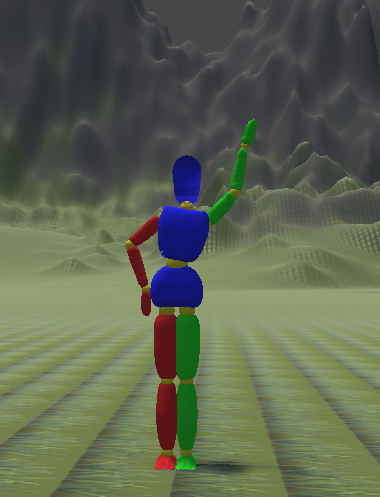
\includegraphics[height=200pt]{dummy.PNG}
    \caption{rig utilizzato per la renderizzazione}
\end{figure}

\subsubsection{classe syncSocketServer}
Questa parte illustra la classe utilizzata per far effettuare allo script in unity la richieta al server centrale dei dati elaborati.

\paragraph{librerie utilizzate}
tale classe è stata implementata nella parte unity e ha richiesto l'importazione di UnityEngine, oltre alle librerie per la comunicazione socket e per la manipolazione dei byte ricevuti dal main server. 
\begin{lstlisting}[style=mycsharp, caption=librerie class client C\#, captionpos=b]
using System;
using System.Net;
using System.Net.Sockets;
using System.Runtime.InteropServices;
using System.Text;
using System.Collections;
using System.Collections.Generic;
using UnityEngine;

\end{lstlisting}

\paragraph{classe client C\# per la comunicazione}
In questa sezione è illustrato la classe che permette la comunicazione con il main server. 
Si noti come l'utilizzo della classe in unity richiede che essa sia figlia della classe MonoBehaviour, interna di unity.
\begin{lstlisting}[style=mycsharp, caption=class client C\#, captionpos=b]

public class SyncSocketClient : MonoBehaviour {
    //struttura union per la conversione Bytes -> float
    [StructLayout(LayoutKind.Explicit)]
    public struct Ubones
    {
        [FieldOffset(0)] public float fBones;
        [FieldOffset(0)] public byte strBones1;
        [FieldOffset(1)] public byte strBones2;
        [FieldOffset(2)] public byte strBones3;
        [FieldOffset(3)] public byte strBones4;
    }

    //Oggetti socket 
    public IPHostEntry ipHostInfo;
    public IPAddress ipAddress;
    public IPEndPoint remoteEP;
    public Socket sender;
    private const int number_of_joints = 2;
    private const int number_of_float = number_of_joints * 3;


    // alloco la struttura di conversione
    public Ubones[] bones = new Ubones[number_of_float]; //4 joints

    // dichiaro il vettore di buffer
    public byte[] bytes;

    //settaggio parametri e inizzializazione comunicazione
    public SyncSocketClient(int Port){ ... }

    //chiusura comunicazione
    public void CloseConnection(){ ... }

    // funzione per la ricezione e la conversione float
    public void ReciveFloat(){ ... }
	
	//funzione per la ricezione della stringa dal server
    public string ReciveString(){ ... }

    //trasmissione stringa
    public void sendMessage(string msg){ ... }

    //funzione di comunicazione, invia il codice di richiesta, riceve i byte li carica nell' union 
    public void TestComunication(){ ... }
	
	//funzione per la reinizializzazione delle variabili bones
    public void initBones(){ ... }
    }
}
\end{lstlisting}

\subsubsection{classe di controllo del manichino}
In questa sezione viene illustrata la classe interna al motore grafico realizzata per il caricamento dei dati ricevuti dal server nella struttura di dell'oggetto 
\paragraph{librerie della classe controllo}
\begin{lstlisting}[style=mycsharp, caption=Librerie classe controllo C\#, captionpos=b]
using System.Collections.Generic;
using System.IO;
using System.Text;
using UnityEngine; 
\end{lstlisting}
\paragraph{corpo della classe controllo}
Anche questa classe è stata resa figlia di MonoBehaviour, il settaggio delle variabili viene effettuat dal metodo Start() richiamato da Unity all'avvio del programma, in questo caso però l'utilizzo della classe è richiamato attivamente da Unity attraverso il metodo Update() che viene richiamato una volta per ogni aggiornamento dello schermo. 
\begin{lstlisting}[style=mycsharp, caption=class client C\#, captionpos=b]
public class ProvaControllo : MonoBehaviour {
	//dichiarazione della classe socketClient sincrono
	//e dell'oggetto di controllo del manichino
    private SyncSocketClient socket;
    public GameObject[] bones;
    
    private List<string> Tags = new List<string>();
    
    /*{ 4, 6, 3, 5, 8};*/ // indici degli oggetti da aggiornare nella lista GameObject  
    public int[] neededObjects = new int[] {3, 5}; 
    
    //ref kinect{ 4, 5, 8, 9}; // indici degli oggetti da aggiornare nella struct Ubones della com socket
    public int[] neededBonesF = new int[] {0, 1}; 
	
	//vettori da tre per il passaggio degli angoli
    public Vector3 BraccioDx;
    public Vector3 avanBraccioDx;
    public Vector3 BraccioSx;
    public Vector3 avanBraccioSx;

    // Metodo di inizializazzione della classe, richiamato all'avvio
    void Start () {
    
    	//attivazione della comunicazione
        socket = new SyncSocketClient(9999);
        
        //inizializazzione della struttura di conversione byte/float
        socket.initBones();
		
		//creazione della lista dei tag
        Tags.Add("Root"); //0
        Tags.Add("Bacino"); //1
        Tags.Add("schiena"); //2
        Tags.Add("BraccioDx"); //3
        Tags.Add("BraccioSx"); //4
        Tags.Add("AvanbraccioDx"); //5
        Tags.Add("AvanbraccioSx"); //6
        Tags.Add("testa"); //7
        Tags.Add("schiena"); //8
        
		//inizializazzione dell'array di oggetti del gioco
        bones = new GameObject[10];
        
        //link degli oggetti creati alle ossa del manichino
        int i = 0;
        foreach (string Tag in Tags) {
            bones[i] = GameObject.FindGameObjectWithTag(Tag);
            i++;
        }
    }
    
	// Update is called once per frame
	void Update () {
		
		//richiesta al server centrsle dei nuovi dati e aggiornamento 
		//della struttura interna alla classe socket
        socket.TestComunication();
		
		//caricamento dei dati ricevuti sulla struttura unity del manichino
        for (int i = 0; i < 2; i++)
        {   
            bones[neededObjects[i]].transform.rotation = Quaternion.Euler(socket.bones[neededBonesF[i]*3].fBones, socket.bones[(neededBonesF[i] * 3) + 1].fBones, socket.bones[(neededBonesF[i] * 3) + 2].fBones);
        }
}

\end{lstlisting}

\section{Conclusioni}
Il progetto in fine si è concluso con esito negativo per quanto riguarda la buona generalizzazione del modello, principalmente a causa della cattiva qualità della bussola 3D, la quale anche durante i test sull'output non filtrato restituiva valori non coincidenti con la realtà.
In compenso la libreria sviluppata per l'addestramento dei modelli ha dato buoni risultati in termini di ottimizzazione dell'addestramento dei modelli, incrementando su GPU la velocità di addestramento di ben 250 volte rispetto alla CPU, risultati soddisfacenti considerando che il programma è affetto fortemente da "race-condition", una problematica che affligge gli approcci al calcolo che si basano fortemente su multithreading.
Tale problematica si presenta quando processi paralleli cercano di eseguire calcoli che mirano a modificare una stessa variabile contemporaneamente, e tale variabile è anche un input di queste funzioni, in particolare un processo prende tale variabile come input copiandola, un altro thread la modifica, e il primo la sovrascrive con il suo risultato non considerando la modifica fatta dal secondo. Per far fronte a tale problema è stato necessario utilizzare le funzioni atomiche che causano un blocco della variabile e mettono in attesa i thread che cercano di utilizzarla, causando una serializzazione delle operazioni.
Un possibile altro approccio sarebbe stato effettuare queste operazioni con uno specifico ordine che mirava a fare più operazioni su più variabili evitando però la race-condition, con tale ottimizzazione si possono raggiungere velocità di computazione molto maggiori, in quanto un solo thread in attesa in un warp in cui tutti gli altri hanno concluso il proprio lavoro, li blocca tutti, e non permette allo stream-multiprocessor di lanciarne un altro.
Abbiamo comunque deciso di non intraprendere questa strada in quanto richiedeva molto tempo e ingenti modifiche alla struttura del programma.\\ 
In oltre con modelli a molti neuroni per layer tendeva ad attenuarsi in quanto si verificavano meno collisioni.
Concludendo il problema non è stato risolto con i risultati sperati, ma la libreria realizzata è perfettamente funzionante e pronta per essere applicata per l'apprendimento di nuove task.


\end{document}